\ifnum \aluno=1
\renewcommand\chapterillustration{abertura-estatistica2}
\else
\renewcommand\chapterillustration{abertura-estatistica2-professor}
\fi 
\renewcommand\chapterwhat{Medidas de posição: média, mediana, moda e quartis. Medidas de dispersão:
desvio médio, variância, desvio padrão, amplitude amostral, distância entre quartis e
coeficiente de variação. Construção do desenho-esquemático (boxplot).} 
\renewcommand\chapterbecause{As medidas resumo (posição e dispersão) correspondem a uma síntese do conjunto de
dados observados e ao passo preliminar para fazer uma inferência estatística, ou seja, a
partir das informações obtidas na amostra, expandir nossas conclusões para a população.
Como as distribuições podem apresentar formas variadas é importante conhecer
diferentes tipos de medidas resumo, tanto de posição como de dispersão, para usar
medidas apropriadas em cada caso.} 
\chapter{Medidas de posição e dispersão}
\label{est2-chap}

\ifdefined\estchapum
\else
\label{est1-chap}
\label{est1-ativ-9}
\label{chap-est1-exerc-17}
\fi
\def\estchapdois{}


\mbox{}\thispagestyle{empty}\clearpage

\thispagestyle{empty}

\begin{center}
Projeto: LIVRO ABERTO DE MATEMÁTICA

\noindent \begin{tabular}{lcccr}K

\includegraphics[scale=.15]{impa}& \quad\quad& 
\includegraphics[width=3cm]{logo} & \quad\quad& 
\includegraphics[scale=.24]{obmep} 
\end{tabular}
\end{center}

\vspace*{.3cm}

Cadastre-se como colaborador no site do projeto: \url{umlivroaberto.org}

Versão digital do capítulo:

\url{https://www.umlivroaberto.org/BookCloud/Volume_1/master/view/PE104.html}

% \begin{center}
%   \includegraphics[width=2cm]{canvas}
% \end{center}

\begin{tabular}{p{.15\textwidth}p{.7\textwidth}}
Título: & Medidas de Posição e Dispersão\\
\\
Ano/ Versão: & 2020 / versão 1.3 de \today\\
\\
Editora & Instituto Nacional de Matem\'atica Pura e Aplicada (IMPA-OS)\\
\\
Realização:& Olimp\'iada Brasileira de Matem\'atica das Escolas P\'ublicas (OBMEP)\\
\\
Produção:& Associação Livro Aberto\\
\\
Coordenação: & Fabio Simas e Augusto Teixeira (livroaberto@impa.br)\\
\\
  Autores: & Flávia Landim (coordenadora da equipe - UFRJ)\\
           & Nei Rocha (UFRJ)\\
           & Vanessa Matos (SEduc Angras dos Reis e Mesquita)\\
           & José Ezequiel Soto
\\
Revisão: &  Letícia Rangel  \\
		 &  Alexandre Silva \\
\\
Design: & Andreza Moreira (Tangentes Design) \\
\\
  Ilustrações: & --- \\ 
\\
Gráficos: & Beatriz Cabral e Tarso Caldas (Licenciandos da UNIRIO)\\
\\
  Capa: & Foto de Clement Chen, no Unsplash\\
  		& https://unsplash.com/photos/EvoIUzuW89s \\

\end{tabular}


\begin{figure}[b]
\begin{minipage}[l]{5cm}
\centering

{\large Licença:}

  
\includegraphics[width=3.5cm]{cc-by-sa1}
\end{minipage}\hfill
\begin{minipage}[c]{5cm}
\centering
{\large Desenvolvido por}


\includegraphics[width=2.5cm]{logo-associacao.jpg}
\end{minipage}
\begin{minipage}[r]{5cm}
\centering

{\large Patrocínio:}
  \vspace{1em}
  
\includegraphics[width=3.5cm]{itau}
\end{minipage}
\end{figure}

\mainmatter

\begin{apresentacao}{Medidas de Posição e Dispersão}

Neste capítulo serão trabalhadas as seguintes habilidades da BNCC para o Ensino Médio:

\begin{habilities}{EM13MAT202}

Planejar e executar pesquisa amostral usando dados coletados ou de diferentes fontes sobre questões relevantes atuais, incluindo ou não, apoio de recursos tecnológicos, e comunicar os resultados por meio de relatório contendo gráficos e interpretação das medidas de tendência central e das de dispersão.

\tcbsubtitle{EM13MAT316} Resolver e elaborar problemas, em diferentes contextos, que envolvem cálculo e interpretação das medidas de tendência central (média, moda, mediana) e das de dispersão (amplitude, variância e desvio padrão).

\tcbsubtitle{EM13MAT408} Construir e interpretar tabelas e gráficos de frequências, com base em dados obtidos em pesquisas por amostras estatísticas, incluindo ou não o uso de softwares que inter-relacionem estatística, geometria e álgebra.

\tcbsubtitle{EM13MAT409} Interpretar e comparar conjuntos de dados estatísticos por meio de diferentes diagramas e gráficos, como o histograma, o de caixa (boxplot), o de ramos e folhas, reconhecendo os mais eficientes para sua análise.

\tcbsubtitle{EM13MAT510} Investigar conjuntos de dados relativos ao comportamento de duas variáveis numéricas, usando tecnologias da informação, e, se apropriado, levar em conta a variação e utilizar uma reta para descrever a relação observada.
\end{habilities}

\subsection{Objetivo Geral do Capítulo}

Compreender como algumas medidas, chamadas medidas resumo, podem revelar informações sobre a distribuição dos dados. Para alcançar este objetivo geral, este capítulo inclui:

\begin{enumerate}
\item definições de medidas de posição (média, mediana, moda e quartis);
\item definições de medidas de dispersão (desvio médio, variância e desvio padrão, amplitude (amostral), distância entre quartis, coeficiente de variação);
\item sinalizações para a importância das medidas de dispersão para avaliar a representatividade da média na distribuição;
\item revisão dos conceitos apresentados no capítulo \hyperref[est1-chap]{\textbf{A Natureza da Estatística}}: parâmetro e estatística, definindo média populacional e média amostral, variância populacional e variância amostral.
\item apresentação de representação gráfica para variáveis quantitativas conhecida como \textit{boxplot} (gráfico caixa).
\end{enumerate}

\textbf{Observação}: Embora muitos textos denominem as medidas de posição (média, mediana e moda) como medidas de tendência central, preferimos denominá-las medidas de posição, pois, por exemplo, na presença de forte assimetria, a média não será um valor central, pois será influenciada pelos valores extremos da distribuição.

\paragraph{Por que estudar o assunto?}

As medidas resumo (posição e dispersão) correspondem a uma síntese do conjunto de dados observados e ao passo preliminar para fazer uma inferência estatística, ou seja, a partir das informações obtidas na amostra, expandir nossas conclusões para a população. Como as distribuições podem apresentar formas variadas é importante conhecer diferentes tipos de medidas resumo, tanto de posição como de dispersão, para usar medidas apropriadas em cada caso.

\paragraph{Desafios do Capítulo}

\begin{enumerate}
\item Entender as especificidades das variadas medidas resumo e reconhecer suas limitações em cada contexto.
\item A partir de algumas medidas resumo, ser capaz de ter uma noção quanto à forma da distribuição dos dados.
\end{enumerate}

\paragraph{Conteúdos abordados}

\begin{enumerate}
\item Medidas de posição: média, mediana, moda e quartis.
\item Medidas de dispersão: amplitude, distância entre quartis, desvio médio, variância, desvio padrão e coeficiente de variação.
\item Parâmetro versus Estimador (estimativa) (Média populacional versus média amostral, Variância populacional versus variância amostral, etc.).
\item Construção do \textit{boxplot} (gráfico caixa).
\end{enumerate}

\paragraph{Pré-requisitos}

\begin{habilities}{EF07MA29} Compreender, em contextos significativos, o significado de média estatística como indicador da tendência de uma pesquisa, calcular seu valor e relacioná-lo, intuitivamente, com a amplitude do conjunto de dados.

\tcbsubtitle{EF08MA22} Obter os valores de medidas de tendência central de uma pesquisa estatística (média, moda e mediana) com a compreensão de seus significados e relacioná-los com a dispersão de dados, indicada pela amplitude.

\tcbsubtitle{EM11MT03} Realizar pesquisas, considerando: o planejamento, a discussão (se será censitária ou por amostra), a seleção de amostras, a elaboração e aplicação de instrumentos de coleta, a organização e representação dos dados (incluindo agrupamentos de dados em classe), a construção de gráficos apropriados (incluindo o histograma), a interpretação e a análise crítica apresentadas em relatórios descritivos.
\end{habilities}

\paragraph{Desdobramentos imediatos}

\begin{habilities}{EM15MT06} Analisar criticamente os métodos de amostragem em relatórios de pesquisas divulgadas pela mídia e as afirmativas feitas para toda a população baseadas em uma amostra.
\end{habilities}

\subsection{Abordagem do Capítulo}

Pretende-se ao longo do capítulo, além de apresentar as definições das variadas medidas, enfatizar suas propriedades. Por exemplo, no caso da média, pretende-se explorar as seguintes propriedades:

\begin{enumerate}
\item a média de um conjunto de números é um valor que pertence ao intervalo delimitado pelos valores extremos deste conjunto (mínimo e máximo);
\item a soma dos desvios da média é sempre zero para qualquer conjunto de números;
\item a média é influenciada por todos os valores no conjunto;
\item a média pode ser um valor que não pertence ao conjunto analisado;
\item a média é um valor representativo do conjunto analisado.
\end{enumerate}

Após definir a média e explorar algumas de suas propriedades, situações em que ela pode ser inadequada como valor representativo de uma distribuição (distribuições com forte assimetria) são apresentadas, motivando assim a definição da mediana, uma medida que é pouco afetada por valores extremos.

Uma vez definidas média e mediana, uma situação em que ambas podem ser consideradas inadequadas como valores representativos de uma distribuição (distribuições bimodais simétricas) é apresentada, motivando assim a definição da moda.

Em adição às medidas de posição, medidas de dispersão complementam a descrição de uma distribuição. A motivação para a necessidade de definir medidas de dispersão será realizada com base em uma atividade em que dois conjuntos de dados apresentam média, mediana e moda coincidentes, mas suas distribuições são diferentes.

Após a definição das medidas de dispersão, uma atividade, na qual dois conjuntos de dados apresentam a mesma variância, é proposta. A finalidade dessa atividade será avaliar a magnitude da variância em relação ao conjunto e definir o coeficiente de variação amostral, usado para avaliar essa magnitude.

Na seção seguinte, será proposta uma atividade para construir uma representação gráfica alternativa ao histograma conhecida como boxplot. O esquema dos cinco números, conjunto formado pelas medidas: mínimo, quartis e máximo é usado na construção do \textit{boxplot}. Os boxplots são gráficos simples e muito usados na comparação de diferentes conjuntos de dados. Na construção do boxplot, é apresentado um critério de classificação de um valor do conjunto como valor atípico em relação aos demais valores do conjunto de dados. Na conclusão desta seção, apresenta-se uma regra empírica para a determinação de frequência de observações nos em intervalos centrados na média de comprimentos dados por dosi desvios padrões e quatro desvios padrões para uma situações nas quais não existem valores atípicos ou estes são raros e, a forma da distribuição não é muito assimétrica.

Na seção \hyperref[\detokenize{PE104-A:sec-para-saber-mais}]{\textbf{Para saber mais}} são apresentadas fórmulas para o cálculo de algumas medidas trabalhadas no capítulo para dados agrupados e algumas demonstrações de resultados trabalhados no capítulo.

Diferencial do Capítulo

De acordo com, Russel e Mokros (1991) \citep[apud][]{batanero2016}, a compreensão da ideia de “valor representativo”{} implica em três competências diferentes:

\begin{enumerate}
\item selecionar o melhor valor representativo para um dado conjunto de dados;
\item construir um conjunto de dados tendo um determinado valor representativo, por exemplo, a moda;
\item compreender o efeito que uma mudança em parte dos dados tem sobre os possíveis valores representativos.
\end{enumerate}
Pretende-se explorar estas três competências nas atividades e exercícios do capítulo.

A fórmula de cálculo da variância é apresentada de forma detalhada para que o aluno compreenda o significado desta medida. No entanto, dada a sua complexidade, evitaremos seu uso direto, propondo o uso da tecnologia para obtê-la.

A definição de quartis e a construção do boxplot são propostas inovadoras em relação ao conteúdo usual de Estatística nos livros didáticos do Ensino Médio. Os conceitos relativamente simples de quartis aliados à grande utilidade do \textit{boxplot} na comparação de grupos diferentes, reforçam a pertinência em tratá-los no Ensino Médio.

\paragraph{Dificuldades típicas dos estudantes (distratores)}

Com base no texto de \citet{batanero2016}, apesar da maior parte dos métodos de análise exploratória de dados envolverem apenas cálculos e interpretações de medidas estatísticas simples, bem como, construções de gráficos e suas respectivas leituras, pesquisadores sugerem que os estudantes apresentam problemas na compreensão de conceitos, e em relacionar os mesmos ao contexto de forma significativa. Uma razão para isso é que, em geral, os professores focam sobre a aplicação de métodos em vez da interpretação de resultados em um dado contexto. Neste texto, um resumo de resultados de pesquisas realizadas neste tema é apresentado. A seguir, algumas destas dificuldades são destacadas.

\begin{enumerate}
\item Cálculo de médias combinadas a partir das médias de diferentes grupos: desprezam-se os tamanhos dos diferentes grupos, calculando uma média simples das médias dos grupos.
\item Cálculo de média para dados agrupados: ignoram-se as frequências, considerando apenas os pontos médios dos intervalos, somando-os e dividindo pelo número de intervalos, ou simplesmente, considerando apenas o valor da variável, quando a variável é quantitativa discreta.
\item Compreensão das medidas de posição: média, mediana e moda.
\item Compreensão das medidas de dispersão, em particular, da variância e do desvio padrão.
\item Interpretação dos valores obtidos no contexto considerado.
\end{enumerate}

Os dois primeiros itens estendem-se para o cálculo da variância e do desvio padrão.

Os distratores serão explorados nas atividades e nos exercícios.

\paragraph{Exemplos}

Princípios norteadores dos exemplos selecionados:

\begin{enumerate}
\item propor problemas cuja solução requer dados a serem coletados pelos alunos ou que de alguma forma estão disponíveis para consulta.
\item contextualizar sempre os problemas propostos, pois o contexto é fundamental nas investigações e interpretações.
\end{enumerate}
\subsection{Estratégia pedagógica}

Usar um processo reflexivo baseado no pensamento estatístico.

\begin{enumerate}
\item Fórmulas e algoritmos para obter as medidas resumo, embora importantes neste capítulo, não serão valorizados.
\item Dar importância à compreensão dos conceitos e à interpretação dos resultados.
\item As atividades deverão estar sempre bem caraterizadas a um problema a ser resolvido em um contexto específico.
\item Neste capítulo, o uso de recursos tecnológicos para a realização dos cálculos de medidas resumo é fundamental. Recomenda-se o GeoGebra e planilhas de cálculo.
\end{enumerate}

O uso de calculadoras é fortemente recomendável. No entanto, cabe alertar o estudante quanto à notação adotada no Brasil para o separador decimal: a vírgula, e que é adotada neste livro. No entanto, a notação utilizada, em geral, nas calculadoras e na maioria dos programas e aplicativos é o ponto decimal. Por exemplo, o GeoGebra usa o ponto como separador de casas decimais e, em geral as planilhas eletrônicas estão formatadas para números, usando a vírgula como separador decimal. Assim, copiar e colar os dados de um aplicativo para outro pode acarretar em grandes variações. Cabe também realçar que é muito importante treinar o estudante a usar corretamente as calculadoras: não é raro, apesar de permitir o uso das mesmas, ocorrerem erros pelo manuseio incorreto da calculadora. O estudante deve ser alertado para a ordem de hierarquia das operações, muito trabalhada nos anos iniciais do segundo segmento do Ensino Fundamental, mas que é aparentemente esquecida quando vão utilizar calculadoras.

Cabe reforçar também que apesar do capítulo poder à primeira vista parecer pesado pelo excesso de definições e fórmulas, é possível verificar que as atividades são relativamente simples e visam muito mais à interpretação das medidas do que o cálculo das mesmas. Sempre serão fornecidas informações para facilitar cálculos quando estes forem solicitados. Nas avaliações, a não ser que seja permitido o uso de calculadora, recomenda-se fortemente não pedir para calcular variâncias e desvios padrões, estes deverão ser, em geral dados, e perguntas envolvendo o significado dos mesmos devem ser feitas.

Enfim o que deve ser valorizado no capítulo é conhecer o significado das medidas aqui apresentadas. O cálculo das mesmas pode ser feito, usando-se aplicativos e, as fórmulas, se por acaso forem necessárias para resolver algum problema, deverão ser sempre fornecidas. Principalmente, em se tratando de medidas de dispersão.

\columnbreak
\raggedcolumns
\subsection{Estrutura do Capítulo}

\subexplore{Explorando 1 - Medidas de Posição}

Nesta seção serão trabalhadas duas atividades. A primeira propõe duas transformações simples nos dados de um conjunto e procura avaliar o efeito destas transformações na distribuição dos dados. A segunda foca especificamente no cálculo de medidas de posição tais como média, mediana e moda, que já devem ser conhecidas do Ensino Fundamental. Também proporemos a divisão do conjunto de dados em quatro intervalos de classes de frequências iguais a 1/4 para definir os três quartis de uma distribuição.

\begin{enumerate}
\item Atividade: Distribuição de notas para perceber o efeito de transformações simples (multiplicação e/ou adição de um valor) no dado na posição e escala(forma) da distribuição, comparando histogramas.
\item Atividade: Apresentação de diferentes conjuntos de dados sobre tempos para completar uma “maratona”{} que apresentam diferentes tipos de assimetria.
\end{enumerate}

\subarrange{Organizando as ideias 1 - Medidas de posição}

Definições de média; mediana; moda e quartis.

\subpractice{Praticando o assunto 1}
Atividades explorando conceitos e propriedades apresentados no organizando as ideias 1.

\subexplore{Explorando 2 - Medidas de dispersão}
Proposição de uma atividade envolvendo dois conjuntos de dados reais, todos com medidas de posição iguais, mas apresentando diferenças em suas distribuições caracterizando a necessidade da medida de dispersão.

\subarrange{Organizando as ideias 2 - Medidas de dispersão}
Definições de amplitude; distância entre quartis; desvio-médio; variância; desvio padrão e coeficiente de variação.

Nesta seção também serão retomados os conceitos de parâmetro e estimador, tratados no capítulo \hyperref[est1-chap]{A Natureza da Estatística} apresentando a definição de variância populacional e amostral, desvio-padrão populacional e amostral e, média populacional e amostral.

Proposição de uma atividade apresentando dois conjuntos de dados com a mesma variância, mas com medidas de posição diferentes para motivar a definição de coeficiente de variação.

\subpractice{Praticando o assunto 2}
Atividades que usam os conceitos e propriedades apresentados no organizando 2 e que buscam dar significado às medidas de dispersão definidas.

\subexplore{Explorando 3}
Proposição de atividade de construção de representação de dados usando Mínimo, $Q_1$, Mediana, $Q_3$ e Máximo.

\subarrange{Organizando as ideias 3}
\begin{enumerate}
\item Definição do boxplot (gráfico caixa) representação gráfica para variáveis quantitativas alternativa ao histograma.
\item Descrição do critério de classificação de um valor como valor atípico do conjunto de dados adotado na construção do boxplot.
\item Apresentação de regra empírica para avaliar a frequência de dados nos intervalos $\bar{x}\pm s$ e $\bar{x}\pm2\cdot s$.
\end{enumerate}

\subpractice{Praticando o assunto 3}
Proposição de atividades de comparação de grupos, usando o boxplot.

\subknow{Para saber mais}

Nesta seção serão apresentadas

\begin{enumerate}
\item fórmulas para o cálculo de medidas apresentadas no capítulo para dados agrupados;
\item demonstrações de propriedades trabalhadas nas seções organizando as ideias;
\end{enumerate}

\subknow{Material Suplementar}

Um applet do GeoGebra foi disponibilizado com manual de instruções nesta seção. Nele será possível gerar conjuntos de dados para os quais serão fornecidas as medidas resumo do conjunto bem como o histograma e o boxplot. Neste applet também será possível entrar com o seu próprio conjunto de dados para obter os gráficos e as medidas resumo.

\subexercise{Exercícios}

Nesta seção são propostos exercícios do ENEM, Vestibulares entre outros, abordando os conteúdos desse capítulo. Nos exercícios serão tratados os distratores.

\textbf{Observação}: Os textos \cite{bussab2017,levine2000,rossman1998} e \cite{triola2005} são recomendados para cursos de estatística a nível de graduação, mas seus capítulos iniciais, que tratam da natureza da estatística, representações gráficas e medidas resumo podem ser úteis. Os mesmos foram consultados para o material deste capítulo.

\end{apresentacao}

\def\currentcolor{session1}
\clearmargin
\clearmargin
\begin{objectives}{Notas de arte}
{
Estudar o efeito de uma transformação simples numa distribuição de dados: adição (posição) ou multiplicação (escala).
}{1}{1}
\end{objectives}
\begin{sugestions}{Notas de arte}
{
Esta atividade tem como objetivo principal levar o aluno a perceber efeitos que certas transformações simples nos dados (adição e multiplicação) acarretam em uma distribuição de frequências e, consequentemente, levá-lo a avaliar possíveis mudanças nas medidas de posição e dispersão que serão tratadas neste capítulo. Como ela é uma atividade introdutória, essas propriedades não serão totalmente exploradas na atividade, mas ao longo da capítulo ela será retomada. Os dados desta atividade podem ser obtidos neste \href{https://www.geogebra.org/m/TNh7dPCf}{link} , e sugere-se o uso do GeoGebra ou uma planilha para realizar as transformações indicadas, embora não seja necessário para a realização da atividade. No item \titem{e)} não há uma resposta certa, mas ele deverá ser explorado futuramente com o objetivo de avaliar os efeitos em uma distribuição quando somamos um valor constante a todos os dados e quando multiplicamos um valor constante a todos os dados.
}{1}{1}
\end{sugestions}
\clearmargin
\begin{answer}{Notas de arte}
{
\begin{enumerate}
\item Analisando o primeiro histograma apresentado com o original, percebe-se que o primeiro apresenta uma pequena alteração com intervalos de classe mais largos, ou seja de comprimento $2{,}4$ (os comprimentos originais dos intervalos são iguais a $2$). Já, o segundo, mantém intervalos de classe com mesmo comprimento aos do original, apresentando um deslocamento dos intervalos em uma unidade para à direita.

\item Com o acréscimo de 1 ponto a cada nota, a nota maior que é $8{,}0$ passa a ser $9{,}0$; já com o aumento de $20\%$ sobre a nota de cada um, a nota maior passa a ser $9{,}6$. Portanto, analisando os dois histogramas dados, conclui-se que o primeiro corresponde ao aumento de $20\%$ na nota de cada um e, o segundo, ao acréscimo de 1 ponto na nota de cada um.

\item Observe que se todos os alunos tiverem o acréscimo de $1$ ponto, a soma total das notas será acrescida de $35$ pontos (pois são $35$ alunos). Ao dividir o total por $35$, perceba que a nova média será alterada exatamente pelo acréscimo de $1$ ponto, passando a ser $6{,}93$. Ou seja, a nova média é dada por $\dfrac{207{,}5+35}{35}\approx5{,}93+1$. Já no caso do aumento de $20\%$ sobre a nota de cada aluno, teremos que a nova soma total de notas será dada pela soma original acrescida de $20\%$ tal que a média será dada por $\dfrac{S+0{,}2\cdot S}{35}=\dfrac{1{,}2\cdot S}{35}=1{,}2\times \underbrace{\frac{S}{35}}_{\mathclap{\approx5{,}9\text{ média original}}}=1{,}2\times5{,}93\approx7{,}12$, em que $S=207{,}5$.

\item Não há uma resposta certa para este item. Se cada aluno olhar o seu ponto de vista particular, para alguns será melhor ganhar um ponto e para outros será melhor ter um aumento de $20\%$ sobre a nota. Mais especificamente, para quem tiver obtido nota $5{,}0$ será indiferente; para quem tiver obtido nota inferior a $5{,}0$ será melhor ganhar um ponto e, para os restantes, será melhor o acréscimo de $20\%$ sobre a nota.
\end{enumerate}
}{1}
\end{answer}
\clearmargin
\begin{objectives}{A maratona}
{
\begin{itemize}
\item Identificar a posição da média e dos quartis no gráfico da distribuição.
\item Apresentar representação gráfica alternativa ao histograma: o \textit{boxplot} sem valores discrepantes.
\end{itemize}
}{1}{1}
\end{objectives}
\begin{sugestions}{A maratona}
{
Nesta atividade serão apresentados conjuntos diferentes de dados envolvendo tempos para completar maratonas. Os dados estão disponíveis neste \href{https://www.geogebra.org/m/ZhqKD9Nz}{link}. Serão fornecidos os totais para que o cálculo das médias envolva apenas uma divisão e possa ser feito com uma calculadora simples. Pretende-se levar o aluno a perceber que na presença de forte assimetria (histograma alongado à direita ou à esquerda), a média pode não ser a medida mais adequada para representar o conjunto e, com isso, motivar a definição de mediana.

É importante discutir as perguntas na caixa Para refletir em sala de aula com o intuito de que os estudantes percebam a necessidade de tratar previamente dados de determinada natureza antes de usá-los numericamente, como é o caso do tempo considerado em unidades distintas (hora:minuto:segundo).

Na sequência se inclui a tabela com a respectiva conversão para minutos em números decimais de modo a simplificar os cálculos na atividade, mas deve-se deduzir com os estudantes como calcular a conversão.

Expressão utilizada para calcular o resultado em minutos decimais (minutos$_{10}$):
\begin{equation*}
\text{minutos}_{10}=\text{Horas}\cdot60+\text{Minutos}+\frac{\text{Segundos}}{60}
\end{equation*}
É importante comentar com os estudantes a diferença observada entre a média e a mediana e que esta se deve a uma forte assimetria na distribuição dos dados, representada pela forma de um histograma alongado para à esquerda com frequências pequenas, tornando a média inferior à mediana.

Sugere-se como atividade interdisciplinar, a realização de corridas com os estudantes na Educação Física, medindo os tempos totais, calculando a velocidade média do percurso e comparando com a velocidade média do primeiro e centésimo lugares da maratona. Recomenda-se explicitar o vínculo com a Física para o cálculo e a interpretação da velocidade média, assim como a colocação de questões críticas que facilitem a interpretação dos resultados, por exemplo, é possível manter essa velocidade média durante quase $3$ horas (tempo médio da maratona de mulheres)?
}{1}{2}
\end{sugestions}
\clearmargin
\marginpar{\vspace{.5em}}
\begin{answer}{A maratona}
{
\begin{enumerate}
\item A tabela com as frequências por intervalo e o histograma ficam de seguinte forma:

\begin{minipage}{.4\linewidth}
\begin{table}[H]
\centering
\setlength\tabcolsep{2.5pt}
\begin{tabular}{|l|c|}
\hline
\tcolor{Intervalo} & \tcolor{Frequência} \\
\hline
$[146{,}0 ; 150{,}0 [$ & $8$ \\
\hline
$[150{,}0 ; 154{,}0 [$ & $5$ \\
\hline
$[154{,}0 ; 158{,}0 [$ & $5$ \\
\hline
$[158{,}0 ; 162{,}0 [$ & $2$ \\
\hline
$[162{,}0 ; 166{,}0 [$ & $5$ \\
\hline
$[166{,}0 ; 170{,}0 [$ & $7$ \\
\hline
$[170{,}0 ; 174{,}0 [$ & $9$ \\
\hline
$[174{,}0 ; 178{,}0 [$ & $16$ \\
\hline
$[178{,}0 ; 182{,}0 [$ & $27$ \\
\hline
$[182{,}0 ; 186{,}0 [$ & $16$ \\
\hline
\end{tabular}
\caption{Guia para o cálculo de frequências do histograma}

\end{table}
\end{minipage}
\begin{minipage}{.59\linewidth}
\begin{figure}[H]
\centering

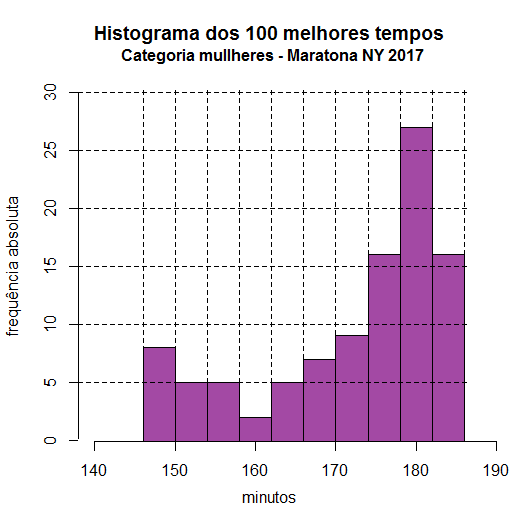
\includegraphics[width=\linewidth]{Histograma_mulheres_resposta_1b.png}
\caption{Histograma dos tempos da categoria de mulheres na Maratona de NY}
\end{figure}
\end{minipage}
\item O tempo médio das primeiras $100$ corredoras é de aproximadamente $171{,}92$ minutos. Uma corredora com esse tempo teria ficado na entre a 35\super{a} e 36\super{a} posição.
\item Para ficar entre os primeiros 25 lugares, uma corredora teria que terminar a corrida em até 165,87 minutos. Já para ficar nas primeiras 50, precisaria terminar o percurso em 176,95 minutos ou menos. Finalmente, para ficar entre as primeiras 75, seu tempo teria que ser menor ou igual a 179,85 minutos.
\begin{figure}[H]
\centering

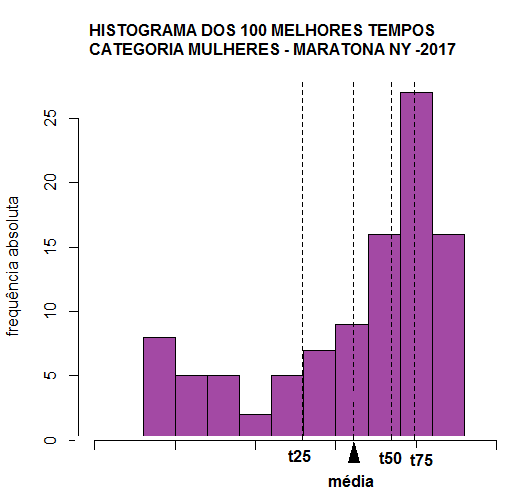
\includegraphics[width=.6\linewidth]{Histograma_mulheres_resposta_1c.png}
\caption{Histograma dos tempos da categoria de mulheres na Maratona de NY mostrando os quartis, a mediana e a média}
\label{}
\end{figure}
\end{enumerate}
}{1}
\end{answer}
\begin{answer}{A maratona}
{
	\begin{enumerate}\setcounter{enumi}{3}
	\item Os comprimentos dos intervalos são dados por:
	\begin{table}[H]
	\centering
	\begin{tabular}{|c|c|}
	\hline
	\tcolor{Intervalo} & \tcolor{Comprimento} \\
	\hline
	1$^{\circ}$ a 25$^{\circ}$ & $18{,}99$ \\
	\hline
	25$^{\circ}$ a 50$^{\circ}$ & $11{,}08$ \\
	\hline
	50$^{\circ}$ a 75$^{\circ}$ & $2{,}90$ \\
	\hline
	75$^{\circ}$ a 100$^{\circ}$ & $5{,}30$ \\
	\hline
	\end{tabular}
	\end{table}

	Lembre-se que se o histograma for construído considerando os intervalos acima, deve-se trabalhar com a escala de densidade de frequência (absoluta ou relativa: razão da frequência pelo comprimento do intervalo), pois os comprimentos dos intervalos são diferentes. No histograma construído nesta atividade, usou-se a escala da frequência absoluta, pois os intervalos considerados têm comprimentos iguais a $4$.
	\item Não coincide com nenhuma delas (25\super{o},50\super{o}, e 75\super{o})

	\item Tem-se que o tempo médio foi $171{,}92$ minutos e o tempo da posição 50 foi $176{,}95$ minutos e, portanto, são diferentes. Adiante vamos trabalhar a razão desta diferença neste conjunto. Isto se deve à forma da distribuição dos tempos de chegada ilustrada pelo histograma. Observando o histograma com as marcações, verifique que a média está em um intervalo de frequência não muito alta ($9$ tempos, com $32$ tempos nos intervalos anteriores e $59$ tempos nos intervalos posteriores), enquanto a o tempo da 50\super{a} posição, mais à direita estão em um intervalo de frequência mais alta ($16$ tempos, com 41 tempos nos intervalos anteriores e $43$ tempos nos intervalos posteriores). Neste caso, o tempo da 50\super{a} posição representa melhor o centro desse conjunto.

	\item Percebe-se uma estrutura com assimetria à esquerda, isto é, frequências baixas (menores ou iguais a 8) nos tempos iniciais ($7$ primeiros intervalos) e grande concentração (frequências altas - maiores ou iguais a $16$) nos três intervalos finais. Esse tipo de estrutura resulta na média inferior ao tempo localizado na posição do meio ($50$ nesse exemplo).

	\item A \hyperref[boxplot-sem-sinalizacao]{figura \ref{boxplot-sem-sinalizacao}} construída é chamada boxplot sem a sinalização de valores discrepantes (vamos chamar de boxplot simplificado). A construção do boxplot com sinalização de valores discrepantes será trabalhada na seção de medidas de dispersão. Veja como fica o boxplot simplificado, adotando-se oreintação horizontal.

	\notas
	{\setcounter{figure}{2}
		\begin{figure}[H]
		\centering
		
		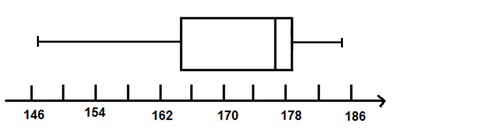
\includegraphics[trim= 0 0 4cm 0, clip,width=.75\linewidth]{bpxplot_Mulheres_maratona_svd.png}
		\caption{Boxplot (sem sinalização de valores discrepantes) dos 100 melhores tempos para a categoria mulheres}
		\label{boxplot-sem-sinalizacao}
		\end{figure}
	}
\setcounter{figure}{3}
	\end{enumerate}
}{1}
\end{answer}
\explore{Medidas de Posição}
\label{\detokenize{PE104-0:sec-explorando1}}\label{\detokenize{PE104-0:explorando-medidas-de-posicao}}\label{\detokenize{PE104-0::doc}}
No capítulo \textbf{\hyperref[est1-chap]{A Natureza Estatística}} trabalhamos com representações gráficas de conjuntos de dados com a finalidade de obter informações sobre estruturas da sua distribuição como estratégia para resumir os dados. No exemplo dos resgistros de tempo deste capítulo, os 64 dados, no quadro a seguir

\begin{table}[H]
\centering
\caption{Registros de tempo de atividade do capítulo \textbf{\hyperref[est1-chap]{A Natureza Estatística}}}
\begin{tabular}{|c|c|c|c|c|c|c|c|}
\hline
\tcolor{A} & \tcolor{B} & \tcolor{C} & \tcolor{D} & \tcolor{E} & \tcolor{F} & \tcolor{G} & \tcolor{H} \\
\hline
3,03 & 4,37 & 5,04 & 5,73 & 4,03 & 5,37 & 6,04 & 6,74 \\ 
\hline
3,38 & 4,46 & 5,11 & 5,84 & 4,38 & 5,46 & 6,11 & 6,84 \\
\hline
3,60 & 4,55 & 5,19 & 5,95 & 4,60 & 5,55 & 6,19 & 6,96 \\ 
\hline
3,78 & 4,63 & 5,29 & 6,08 & 4,78 & 5,64 & 6,29 & 7,08 \\
\hline
3,92 & 4,71 & 5,36 & 6,23 & 4,92 & 5,72 & 6,36 & 7,23 \\
\hline
4,04 & 4,79 & 5,45 & 6,41 & 5,04 & 5,79 & 6,45 & 7,40 \\
\hline
4,16 & 4,87 & 5,54 & 6,62 & 5,16 & 5,87 & 6,54 & 7,63 \\
\hline
4,27 & 4,95 & 5,64 & 6,97 & 5,26 & 5,95 & 6,64 & 7,97 \\ 
\hline
\end{tabular}
\end{table}

foram organizados em 10 intervalos de classe, como mostra a tabela a seguir

\begin{table}[H]
\centering
\caption{Registros de tempo agrupados em intervalos de classe}
\label{\detokenize{PE104-0:id4}}
\begin{tabular}{|l|c|}
\hline
\tcolor{Intervalo de classe} & \tcolor{Número de observações} \\
\hline
{[} 3,0 ; 3,5 {[} & 2 \\
\hline
{[} 3,5 ; 4,0 {[} & 3 \\ 
\hline
{[} 4,0 ; 4,5 {[} & 7 \\
\hline
{[} 4,5 ; 5,0 {[} & 9 \\
\hline
{[} 5,0 ; 5,5 {[} & 11 \\
\hline
{[} 5,5 ; 6,0 {[} & 11 \\ 
\hline
{[} 6,0 ; 6,5 {[} & 9 \\ 
\hline
{[} 6,5 ; 7,0 {[} & 7 \\ 
\hline
{[} 7,0 ; 7,5 {[} & 3 \\
\hline
{[} 7,5 ; 8,0 {[} & 2 \\ 
\hline
\end{tabular}
\end{table}


que, por sua vez, foi usada para construir um gráfico, o histograma a seguir.

\begin{figure}[H]
\centering
\capstart

\begin{tikzpicture}
\begin{scope}[x=60, y = 15]
\matrix[column sep=0.5cm, row sep=0.5cm]{
	\draw (3,0) -- (8,0);
	\foreach \ye in {0,...,12}{
		\draw [help lines, lightgray] (2.5,\ye) -- (8.5,\ye);
		\node [left] at (2.5,\ye) {\ye} ;
	}
	\foreach \xl/ \xr/\y in {3.0/3.5/2,3.5/4.0/3,4.0/4.5/7,4.5/5.0/9,5.0/5.5/11,5.5/6.0/11,6.0/6.5/9,6.5/7.0/7,7.0/7.5/3,7.5/8.0/2}{
	\draw [fill=\currentcolor!80] (\xl,0) rectangle (\xr,\y);
	\node [right, rotate=270] at ($(\xl,0)!0.5!(\xr,0)$) {\xl  a \xr};
	}
	\filldraw[fill=gray] (5.5,0) -- (5.4,-3) -- (5.6,-3) -- cycle;
	\node [below] at (5.5,-3) {média};
\\};
\end{scope}
\end{tikzpicture}
\caption{Histograma dos registros de tempo}\label{\detokenize{PE104-0:fig-histograma-resposta}}\label{\detokenize{PE104-0:id5}}

\end{figure}

Observe que os 64 registros de tempo foram resumidos numa representação gráfica que revela o comportamento destes dados: registros de tempo entre $3{,}0$ e $8{,}0$, estrutura simétrica em torno da média dos resgistros de tempo que é $5{,}5$.

O capítulo \textbf{Medidas de Posição e Dispersão} tem como objetivo responder, entre outras, as seguintes perguntas sobre um conjunto de dados quantitativos.
\begin{enumerate}
\item {} 
É possível encontrar valor(es) para resumir as observações? Qual(is) seria(m) este(s) valor(es)? Como encontrá-lo(s)?

\item {} 
Como medir se os dados estão “próximos”{} ou “afastados”{} uns dos outros?

\item {} 
Como você classifica a forma do gráfico construído para representar os dados?

\item {} 
Existe algum valor muito diferente dos demais? Como identificá-lo?

\end{enumerate}

Ao longo deste capítulo veremos como resumir a informação dos dados, usando apenas algumas medidas que caracterizam a distribuição em vez de usar toda a coleção de dados para descrevê-la. Por esta razão, tais medidas são chamadas medidas resumo.

Como as distribuições podem apresentar formas variadas é importante conhecer diferentes tipos de medidas resumo, tanto de posição como de dispersão, para usar medidas apropriadas em cada caso.

\clearpage

\phantomsection\label{\detokenize{PE104-0:ativ-notas-de-artes}}
\begin{task}{ notas de Artes}

Ao final de um trimestre, um professor de Artes registrou as seguintes notas de seus 35 alunos, listadas no quadro a seguir, em ordem crescente.

\begin{table}[H]
\centering
\begin{tabular}{|c|c|c|c|c|c|c|}
\hline
0,8 & 20 & 2,0 & 2,5 & 2,5 & 3,5 & 4,5 \\
\hline
5,0 & 5,4 & 5,5 & 5,5 & 5,5 & 6,0 & 6,0 \\
\hline
6,0 & 6,0 & 6,3 & 6,5 & 6,8 & 6,8 & 7,0 \\
\hline
7,0 & 7,0 & 7,0 & 7,3 & 7,3 & 7,5 & 7,5 \\
\hline
7,5 & 7,5 & 7,8 & 8,0 & 8,0 & 8,0 & 8,0 \\
\hline
\end{tabular}
\end{table}

Este professor verificou que a média da turma foi aproximadamente $5{,}93$ (soma das notas \(S=207,5\)). Como a participação da turma foi muito boa ao longo do trimestre, o professor resolveu dar uma bonificação na nota de cada aluno desta turma, pensando em duas possibilidades:

\begin{itemize}
\item {} 
acrescentar um ponto para cada aluno da turma;

\item {} 
aumentar em $20\%$ a nota de cada aluno da turma.
\end{itemize}


A \hyperref[tabela-notas1]{tabela \ref{tabela-notas1}} contém os intervalos de classe considerados na construção do histograma das notas sem bonificação, ilustrado na \hyperref[figura-notas1]{figura \ref{figura-notas1}}

\begin{table}[H]
\centering
\caption{Distribuição de frequências das notas antes de bonificação}
\label{tabela-notas1}
\begin{tabular}{|l|c|}
\hline
\tcolor{Intervalo} & \tcolor{Frequência absoluta} \\
\hline
${[}0{,}2{[}$ & $1$ \\
\hline
${[}2{,}4{[}$ & $5$ \\
\hline
${[}4{,}6{[}$ & $6$ \\ 
\hline
${[}6{,}8{]}$ & $23$ \\
\hline
\end{tabular}
\end{table}

\begin{figure}[H]
\centering

\begin{tikzpicture}
\begin{scope}[x=10, y = 5]
\matrix[column sep=0.5cm, row sep=0.5cm]{
	\foreach \ye in {0,5,...,25}{
		\draw [help lines, lightgray] (-0,\ye) -- (10,\ye);
		\draw (0,\ye) -- (-0.4,\ye);
		\node [left] at (-0.4,\ye) {\ye} ;
	}
	\draw (-0.5,0) -- (10,0);
	\draw (0,0) -- (0,25);
	\foreach \xl/ \xr/\y in {0/2/1,2/4/5,4/6/6,6/8/23}{
	\draw [fill=\currentcolor!80] (\xl,0) rectangle (\xr,\y);
	%\node [right, rotate=270] at ($(\xl,0)!0.5!(\xr,0)$) {$\xl$  a $\xr$};
	}
	\foreach \x in {0,2,...,10}{
		\draw (\x,0) -- (\x,-0.4);
		\node [below] at (\x,-0.4) {\x};
	}
\node [rotate=90] at (-4,12.5) {Frequencia absoluta};
\node [below] at (5,-4) {Notas};
%	\filldraw[fill=destacado] (5.5,0) -- (5.4,-3) -- (5.6,-3) -- cycle;
%	\node [below] at (5.5,-3) {média};

\\};
\end{scope}

\end{tikzpicture}
\caption{Histograma das notas de Artes sem bonificação}\label{\detokenize{PE104-0:fig-histograma-notas-sem-bonificacao}}\label{figura-notas1}\end{figure}

Os dois histogramas a seguir, na \hyperref[figura-notas2]{figura \ref{figura-notas2}} correspondem às notas, após usar cada uma das possibilidades consideradas pelo professor, mantendo quatro intervalos de classe, conforme as \hyperref[tabela-notas2]{tabelas \ref{tabela-notas2} e \ref{tabela-notas3}} .

\begin{figure}[H]
\centering
\begin{minipage}{0.4\textwidth}
\begin{tikzpicture}
\begin{scope}[x=10, y = 5]


	\foreach \ye in {0,5,...,25}{
		\draw [help lines, lightgray] (-0,\ye) -- (10,\ye);
		\draw (0,\ye) -- (-0.4,\ye);
		\node [left] at (-0.4,\ye) {\ye} ;
	}
	\draw (-0.5,0) -- (10,0);
	\draw (0,0) -- (0,25);
	\foreach \xl/ \xr/\y in {0/2/1,2/4/5,4/6/6,6/8/23}{
	\draw [fill=\currentcolor!80] (1.2*\xl,0) rectangle (1.2*\xr,\y);
	%\node [right, rotate=270] at ($(\xl,0)!0.5!(\xr,0)$) {$\xl$  a $\xr$};
	}
	\foreach \x in {0,2,...,10}{
		\draw (\x,0) -- (\x,-0.4);
		\node [below] at (\x,-0.4) {\x};
	}
\node [rotate=90] at (-4,12.5) {Frequencia absoluta};
\node [below] at (5,-4) {($\quad$)};
%	\filldraw[fill=destacado] (5.5,0) -- (5.4,-3) -- (5.6,-3) -- cycle;
%	\node [below] at (5.5,-3) {média};

\end{scope}
\end{tikzpicture}
\end{minipage}
\begin{minipage}{0.4\textwidth}
\begin{tikzpicture}
\begin{scope}[x=10, y = 5]



	\foreach \ye in {0,5,...,25}{
		\draw [help lines, lightgray] (-0,\ye) -- (10,\ye);
		\draw (0,\ye) -- (-0.4,\ye);
		\node [left] at (-0.4,\ye) {\ye} ;
	}
	\draw (-0.5,0) -- (10,0);
	\draw (0,0) -- (0,25);
	\foreach \xl/ \xr/\y in {0/2/1,2/4/5,4/6/6,6/8/23}{
	\draw [fill=\currentcolor!80] (\xl+1,0) rectangle (\xr+1,\y);
	%\node [right, rotate=270] at ($(\xl,0)!0.5!(\xr,0)$) {$\xl$  a $\xr$};
	}
	\foreach \x in {0,2,...,10}{
		\draw (\x,0) -- (\x,-0.4);
		\node [below] at (\x,-0.4) {\x};
	}
\node [rotate=90] at (-4,12.5) {Frequencia absoluta};
\node [below] at (5,-4) {($\quad$)};

%	\filldraw[fill=destacado] (5.5,0) -- (5.4,-3) -- (5.6,-3) -- cycle;
%	\node [below] at (5.5,-3) {média};

\end{scope}
\end{tikzpicture}
\end{minipage}

\caption{Histogramas das notas de Artes com bonificação}\label{\detokenize{PE104-0:fig-histogramas-notas-aleteradas}}
\label{figura-notas2}
\end{figure}

\begin{table}[H]
\centering
\caption{Distribuição de frequências das notas após acréscimo de 1 ponto a cada nota}
\label{tabela-notas2}
\begin{tabular}{|l|c|}
\hline
\tcolor{Intervalo} & \tcolor{Frequência absoluta} \\
\hline
${[}1;3{[}$ & $1$ \\
\hline
${[}3;5{[}$ & $5$ \\
\hline
${[}5;7{[}$ & $6$ \\
\hline
${[}7;9{]}$ & $23$ \\
\hline
\end{tabular}
\end{table}
\begin{table}[H]
\centering
\caption{Distribuição de frequências das notas após aumento de 20\% sobre a nota}
\label{tabela-notas3}
\begin{tabular}{|l|c|}
\hline
\tcolor{Intervalo} & \tcolor{Frequência absoluta} \\
\hline
${[}0 ; 2{,}4{[}$ & $1$ \\
\hline
${[}2{,}4 ; 4{,}8{[}$ & $5$ \\
\hline
${[}4{,}8 ; 7{,}2{[}$ & $6$ \\ 
\hline
${[}7{,}2 ; 9{,}6{]}$ & $23$ \\
\hline
\end{tabular}
\end{table}

\begin{enumerate}
\item {} 
Compare os histogramas das notas com bonificação com o histograma original. O que mudou em cada um deles em relação ao original?


\item {} 
Considerando os \hyperref[\detokenize{figura-notas2}]{Histogramas das notas de Artes com bonificação}, identifique qual deles corresponde ao  acréscimo de $1{,}0$ ponto, assinalando (a) e qual deles corresponde ao aumento de $20\%$ das notas originais, assinalando (b).

\item {} 
Dada a informação inicial de que a média da turma foi $5{,}93$, de quanto será a média se o professor acrescentar um ponto a cada aluno? E se ele aumentar em $20\%$ a nota de cada aluno?

\item {} 
Se você fosse um aluno desta turma, que possibilidade de bonificação você escolheria? Para que notas é melhor cada uma das estratégias?

\end{enumerate}
\end{task}


\phantomsection\label{\detokenize{PE104-0:ativ-maratona-de-ny}}
\begin{task}{ a maratona}

A maratona é uma prova de atletismo que consiste em correr uma distância de $42{,}195$km. Pelas suas características, este tipo de prova é realizada nas ruas de uma grande cidade ou na estrada. As principais cidades do mundo realizam um destes eventos anualmente, recebendo milhares de atletas profissionais e amadores que encaram o desafio e almejam finalizar a corrida ou melhorar o próprio tempo do passado.

Uma das mais famosas é a Maratona da Cidade de Nova Iorque, nos Estados Unidos. Veja na figura \hyperref[\detokenize{PE104-0:fig-maratona-ny}]{Corredores participando da Maratona de Nova York, Wikipedia} realização de uma maratona em Nova Iorque. Com mais de 50.000 participantes cada ano, é um dos principais eventos do atletismo mundial, junto com as maratonas de Chicago, Londres, Boston, Berlim e Tóquio.

\begin{figure}[H]
\centering

\includegraphics[width=200bp]{{New_York_marathon_Verrazano_bridge}.jpg}
\caption{Corredores participando da Maratona de \textit{Nova York}, 
\href{https://commons.wikimedia.org/wiki/File:New\_York\_marathon\_Verrazano\_bridge.jpg}{Wikipedia}}
\label{\detokenize{PE104-0:fig-maratona-ny}}
\label{\detokenize{PE104-0:id11}}
\end{figure}

Os resultados do evento são divididos nas categorias de homens e mulheres, além disso, no evento participam cadeirantes e pessoas usando triciclos de mão (\textit{handcycle}), categorias cujos resultados são premiados e publicados separadamente. Qual das categorias você acha que terá os melhores resultados na maratona? Em quanto tempo você acha que uma pessoa percorre os 42,195 km? O que você acha ser mais rápido: correr em cadeira de rodas ou em triciclo de mão?

\phantomsection\label{\detokenize{PE104-0:handcycle}}
\begin{figure}[H]
\centering
\includegraphics[width=200bp]{{Handcycle_in_Richmond_Park_-_geograph.org.uk_-_1315077}.jpg}
\label{\detokenize{PE104-0:handcycle}}
\end{figure}

A seguir analisaremos os tempos de corrida das 100 melhores atletas na categoria de Mulheres da Maratona de Nova York do ano 2017, dados disponíveis no \href{http://results.nyrr.org/event/M2017/finishers}{site oficial da competição}.

Observe no quadro a seguir, que os tempos já estão ordenados do menor para o maior e que para identificar o tempo da quadragésima sétima chegada, basta tomar a interseção da linha $7$ com a coluna $+40$ para obter o tempo $2:55:36$, ou seja, duas horas $55$ minutos e $36$ segundos.



\begin{table}[H]
\centering
\caption{100 melhores tempos de finalização da Maratona de Nova Iorque 2017 para mulheres (hora:minuto:segundo)}
\setlength\tabcolsep{2.5pt}
\label{\detokenize{PE104-0:id12}}
\begin{tabular}{|c|r|r|r|r|r|r|r|r|r|r|}
\hline
\tcolor{}& \tcolor{+0} & \tcolor{+10} & \tcolor{+20} & \tcolor{+30} & \tcolor{+40} & \tcolor{+50} & \tcolor{+60} & \tcolor{+70} & \tcolor{+80} & \tcolor{+90} \\
\hline
1 & 2:26:53 & 2:32:01 & 2:42:52 & 2:49:44 & 2:53:59 & 2:56:58 & 2:58:35 & 2:59:36 & 3:01:24 & 3:03:43 \\
\hline
2 & 2:27:54 & 2:32:09 & 2:44:26 & 2:49:59 & 2:54:42 & 2:57:05 & 2:58:36 & 2:59:41 & 3:01:26 & 3:03:46 \\
\hline
3 & 2:28:08 & 2:33:18 & 2:44:48 & 2:50:04 & 2:54:52 & 2:57:10 & 2:58:50 & 2:59:43 & 3:01:28 & 3:04:02 \\
\hline
4 & 2:29:36 & 2:34:10 & 2:45:20 & 2:50:05 & 2:55:04 & 2:57:40 & 2:58:52 & 2:59:46 & 3:01:44 & 3:04:04 \\
\hline
5 & 2:29:39 & 2:34:23 & 2:45:52 & 2:51:11 & 2:55:25 & 2:57:49 & 2:58:56 & 2:59:51 & 3:02:09 & 3:04:17 \\
\hline
6 & 2:29:39 & 2:36:38 & 2:46:45 & 2:53:01 & 2:55:34 & 2:57:49 & 2:59:01 & 2:59:56 & 3:02:15 & 3:04:26 \\
\hline
7 & 2:29:41 & 2:37:22 & 2:47:04 & 2:53:02 & 2:55:36 & 2:57:50 & 2:59:03 & 3:00:02 & 3:02:39 & 3:04:42 \\
\hline
8 & 2:29:56 & 2:37:33 & 2:47:30 & 2:53:02 & 2:55:39 & 2:58:08 & 2:59:10 & 3:00:05 & 3:02:41 & 3:04:49 \\
\hline
9 & 2:31:21 & 2:39:01 & 2:47:35 & 2:53:19 & 2:56:47 & 2:58:23 & 2:59:16 & 3:00:49 & 3:02:56 & 3:04:58 \\
\hline
10 & 2:31:44 & 2:40:09 & 2:49:37 & 2:53:38 & 2:56:57 & 2:58:26 & 2:59:23 & 3:01:18 & 3:03:32 & 3:05:09 \\
\hline
\end{tabular}
\end{table}


\begin{reflection}
\begin{itemize}
\item {} 
Como você calcularia a média de valores em horas, minutos e segundos,  como os da tabela?

\item {} 
Como você construiria um histograma com estes dados? Como você definiria os limites dos intervalos? (Consulte a atividade \hyperref[est1-ativ-9]{Construção do Histrograma} do capítulo \textbf{\hyperref[est1-chap]{A Natureza Estatística}} em caso de dúvida.)

\item {} 
Qual o maior tempo em que uma corredora deveria completar a maratona para ficar entre as 25 primeiras? E entre as 50 primeiras?

\end{itemize}
\end{reflection}

Para calcular a média destes dados é conveniente reduzi-los a uma única unidade de medida, pois, caso contrário, seria necessário calcular três médias e, ainda fazer conversões apropriadas para obter a resposta em hora:minuto:segundo. Convertendo todos os tempos para minutos, obtemos o seguinte quadro de tempos arredondados para duas casas decimais.

\begin{table}[H]
\centering
\setlength\tabcolsep{3.5pt}
\begin{tabular}{|c|r|r|r|r|r|r|r|r|r|r|}
\hline
\tcolor{}& \tcolor{+0} & \tcolor{+10} & \tcolor{+20} & \tcolor{+30} & \tcolor{+40} & \tcolor{+50} & \tcolor{+60} & \tcolor{+70} & \tcolor{+80} & \tcolor{+90} \\
\hline
1 & 146,88 & 152,02 & 162,87 & 169,73 & 173,98 & 176,97 & 178,58 & 179,60 & 181,40 & 183,72 \\
\hline
2 & 147,90 & 152,15 & 164,43 & 169,98 & 174,70 & 177,08 & 178,60 & 179,68 & 181,43 & 183,77 \\ 
\hline
3 & 148,13 & 153,30 & 164,80 & 170,07 & 174,87 & 177,17 & 178,83 & 179,72 & 181,47 & 184,03 \\
\hline
4 & 149,60 & 154,17 & 165,33 & 170,08 & 175,07 & 177,67 & 178,87 & 179,77 & 181,73 & 184,07 \\
\hline
5 & 149,65 & 154,38 & 165,87 & 171,18 & 175,42 & 177,82 & 178,93 & 179,85 & 182,15 & 184,28 \\
\hline
6 & 149,65 & 156,63 & 166,75 & 173,02 & 175,57 & 177,82 & 179,02 & 179,93 & 182,25 & 184,43 \\
\hline
7 & 149,68 & 157,37 & 167,07 & 173,03 & 175,60 & 177,83 & 179,05 & 180,03 & 182,65 & 184,70 \\
\hline
8 & 149,93 & 157,55 & 167,50 & 173,03 & 175,65 & 178,13 & 179,17 & 180,08 & 182,68 & 184,82 \\
\hline
9 & 151,35 & 159,02 & 167,58 & 173,32 & 176,78 & 178,38 & 179,27 & 180,82 & 182,93 & 184,97 \\
\hline
10 & 151,73 & 160,15 & 169,62 & 173,63 & 176,95 & 178,43 & 179,38 & 181,30 & 183,53 & 185,15 \\
\hline
\end{tabular}
\end{table}

\begin{enumerate}
\item {} 
Construa um histograma dos dados convertidos para horas, completando a \hyperref[tabela-maratona3]{tabela \ref{tabela-maratona3}}, que indica os intervalos de classe (fechados no limite inferior e abertos no limite superior).

\begin{table}[H]
\centering
\begin{tabular}{|l|c|}
\hline
\tcolor{Intervalo} & \tcolor{Frequência} \\
\hline
$[146{,}0 ; 150{,}0 [$ & \\
\hline
$[150{,}0 ; 154{,}0 [$ & \\
\hline
$[154{,}0 ; 158{,}0 [$ & \\
\hline
$[158{,}0 ; 162{,}0 [$ & \\
\hline
$[162{,}0 ; 166{,}0 [$ & \\
\hline
$[166{,}0 ; 170{,}0 [$ & \\
\hline
$[170{,}0 ; 174{,}0 [$ & \\
\hline
$[174{,}0 ; 178{,}0 [$ & \\
\hline
$[178{,}0 ; 182{,}0 [$ & \\
\hline
$[182{,}0 ; 186{,}0 [$ & \\
\hline
\end{tabular}
\caption{Intervalos de classes}
\label{tabela-maratona3}
\end{table}
% \begin{figure}[H]
% \centering
% \capstart

% \begin{tikzpicture}[scale=.8, every node/.style={scale=.8}]
% \begin{scope}[x=500, y = 7]
% 	\foreach \ye in {0,2,...,30}{
% 		\draw [help lines, lightgray] (2.4480,\ye) -- (3.0860,\ye);
% 		\draw (2.4480,\ye) -- (2.435,\ye);
% 		\node [left] at (2.435,\ye) {\ye} ;
% 	}
% 	\foreach \xe in {2.4480,2.5118,2.5756,2.6394,2.7032,2.7670,2.8308,2.8946,2.9584,3.0222,3.0860}{
% 		\draw [help lines, lightgray] (\xe,0) -- (\xe,30);
% 		\draw (\xe,0) -- (\xe,-1);
% 		\node [right,rotate=-90] at (\xe,-1) {\xe} ;
% 	}
% 	\draw (2.4480,30) -- (2.4480,0) -- (3.0860,0);
% %	\filldraw[fill=destacado] (5.5,0) -- (5.4,-3) -- (5.6,-3) -- cycle;
% %	\node [below] at (5.5,-3) {média};
% \end{scope}

% \end{tikzpicture}\caption{Eixos para a construção do histograma}\label{\detokenize{PE104-0:hist-maratona-mulheres}}\label{\detokenize{PE104-0:id15}}\end{figure}

\item {} 
Calcule o tempo médio dos 100 melhores tempos das corredoras, sabendo que a soma dos tempos é $17.191{,}66$ minutos. Localize o valor encontrado no eixo horizontal do histograma. Em que posição ficaria uma corredora cujo tempo no qual completou a maratona é igual ao tempo médio calculado neste item?


\item {} 
Trace linhas verticais no histograma de modo a separar as classificações em 4 grupos: uma linha vertical que identifica o 25$^{\circ}$ lugar, separando os 25 primeiros colocados dos demais; outra, que identifica a 50$^{\text{a}}$ classificação e, por fim, uma que marca o 75$^{\circ}$ tempo na classificação geral.

As marcações dos tempos das 25$^{\text{a}}$, 50$^{\text{a}}$ e 75$^{\text{a}}$ posições neste conjunto de 100 observações são chamadas de quartis da distribuição, este conceito será formalizado adiante.

\newpage
\item {} 
Calcule os comprimentos dos intervalos de tempo determinados pela proposta de divisão no item \titem{d)} e compare-os.

\begin{table}[H]
\centering
\begin{tabular}{|c|c|}
\hline
\tcolor{Intervalo} & \tcolor{Comprimento} \\
\hline
1$^{\circ}$ a 25$^{\circ}$ & \\
\hline
25$^{\circ}$ a 50$^{\circ}$ & \\
\hline
50$^{\circ}$ a 75$^{\circ}$ & \\
\hline
75$^{\circ}$ a 100$^{\circ}$ & \\
\hline
\end{tabular}
\end{table}

Observa-se que os comprimentos dos intervalos são bem diferentes, sendo maiores no início e mais estreitos no final.

Observe que apesar das diferenças de comprimento desses intervalos, cada um deles corresponde a cerca de 25 tempos.

\item {} 
O valor obtido para o tempo médio coincide com alguma das outras marcas feitas no histograma?

\item {} 
Observe que o tempo médio dos 100 melhores tempos para mulheres e o tempo da corredora que chegou em 50\super{o}. lugar são diferentes. Qual deles você escolheria como medida resumo destes dados? Por quê?

\item Que características da distribuição dos 100 melhores tempos para mulheres podem ser destacadas, analisando-se o histograma construído?

(Construção de boxplot simplificado) Considerando os valores mínimo ($146{,}88$ min.) e máximo ($185{,}15$ min.), trace uma reta (vertical ou horizontal), incluindo esse intervalo de variação. Por exemplo, de $146$ a $186$.
\begin{figure}[H]
\centering


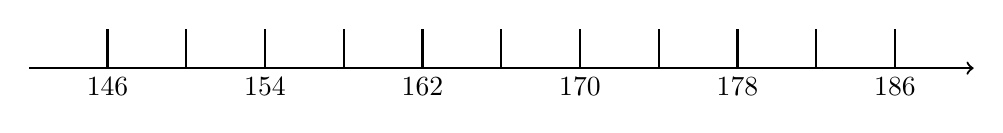
\begin{tikzpicture}
\draw [->,thick] (0,0) -- (12,0);
\foreach \x in {1,...,11} \draw [thick] (\x,0) -- (\x,.5);
\foreach \x/\y in {1/146,3/154,5/162,7/170,9/178,11/186} \node [below] at (\x,0) {$\y$};
\end{tikzpicture}
\caption{Sugestão de escala para a construção do boxplot dos 100 melhores tempos (em minutos) para a categoria mulheres}
\label{}
\end{figure}

Em seguida, trace um retângulo, cujas bases estão nas posições referentes aos 25º e 75º tempos de chegada, cortando o retângulo por um segmento na posição referente ao 50º tempo de chegada. Para terminar a construção, trace um segmento, partindo do ponto médio da parte inferior até o valor mínimo e repita para o ponto médio da parte superior até o valor máximo.

A figura obtida é conhecida como boxplot (gráfico-caixa) do 100 melhores tempos sem a sinalização de valores discrepantes.

O boxplot é uma representação gráfica de dados quantitativos alternativa ao histograma. Esse gráfico é útil na comparação do comportamento de uma variável, considerando diferentes grupos, por exemplo, 100 melhores tempos de chegada entre homens e mulheres.
\end{enumerate}
\end{task}


\arrange{Medidas de Posição}
\label{\detokenize{PE104-1:sec-organizando1}}\label{\detokenize{PE104-1::doc}}\label{\detokenize{PE104-1:organizando-as-ideias-medidas-de-posicao}}

Medidas de Posição, como o próprio termo indica, visam a resumir um conjunto de dados em geral numa única medida em algum lugar geométrico entre os extremos observados do conjunto (mínimo e máximo). Veja na \hyperref[\detokenize{PE104-1:fig-coloque-aqui-o-nome}]{figura \ref{\detokenize{PE104-1:fig-coloque-aqui-o-nome}}}, as marcações da média e da mediana das notas de Artes sem bonificação.

\begin{figure}[H]
\centering
\capstart

\begin{tikzpicture}
\begin{scope}[x=15, y = 5]
	\foreach \ye in {0,5,...,25}{
		\draw [help lines, lightgray] (-0,\ye) -- (10,\ye);
		\draw (0,\ye) -- (-0.4,\ye);
		\node [left] at (-0.4,\ye) {\ye} ;
	}
	\draw (-0.5,0) -- (10,0);
	\draw (0,0) -- (0,25);
	\foreach \xl/ \xr/\y in {0/2/1,2/4/5,4/6/6,6/8/23}{
	\draw [ thick, fill=\currentcolor!80] (\xl,0) rectangle (\xr,\y);
	%\node [right, rotate=270] at ($(\xl,0)!0.5!(\xr,0)$) {$\xl$  a $\xr$};
	}
	\foreach \x in {0,2,...,10}{
		\draw (\x,0) -- (\x,-0.4);
		\node [below] at (\x,-0.4) {\x};
	}
\node at (5, 30) {Histograma das notas de Artes};
\node [rotate=90] at (-3,12.5) {Frequencia absoluta};
\node [below] at (5,-4) {Notas};
\draw [color=destacado, very thick, dashed] (5.91,-0.4) -- (5.91,27);
\node [left, color=destacado] at (5.91,27) {média};
\draw [color=atento, very thick, dashed] (6.5,-0.4) -- (6.5,27);
\node [right, color=atento] at (6.5,27) {mediana};
%	\filldraw[fill=destacado] (5.5,0) -- (5.4,-3) -- (5.6,-3) -- cycle;
%	\node [below] at (5.5,-3) {média};
\end{scope}

\end{tikzpicture}
\caption{Média e mediana assinaladas no Histograma de das notas de Artes}\label{\detokenize{PE104-1:fig-coloque-aqui-o-nome}}\label{\detokenize{PE104-1:id6}}\end{figure}

Só é possível obter medidas como a média e a mediana, se nossas observações são de natureza quantitativa, pois, como vimos no capítulo
\textbf{\hyperref[est1-chap]{A Natureza Estatística}}, as variáveis qualitativas estão no domínio da frequência apenas, ou seja, só podemos contar quantas observações ocorrem em cada categoria da variável qualitativa, mas não podemos operar matematicamente com as categorias em si. Por exemplo, na atividade Prática de Atividades Físicas deste capítulo, trabalhamos com a variável modalidade do esporte praticado. As modalidades correspondem à “Futebol”, “Caminhada”, “Fitness”, etc. Observe que são respostas não numéricas e, por isso, não podemos calcular uma média e não existe uma relação de ordem natural das respostas. Apenas podemos ordenar as respostas pela frequência na qual elas ocorreram.

As principais medidas de posição usadas na Estatística são a média, a mediana, a moda e os quartis da distribuição. Lembre-se que essas medidas buscam de alguma forma resumir a informação do conjunto.

Para definir as medidas a serem estudadas neste capítulo vamos adotar a notação descrita no exemplo a seguir.

\begin{example}{Idade de pessoas que tomaram a vacina da febre amarela}

Suponha que na primeira segunda-feira do mês de março de 2018, um Posto de Saúde tenha registrado as idades (em anos completos) das seis primeiras pessoas que chegaram para tomar a vacina da febre amarela e, os registros, obtidos foram \(\{55, 22, 30, 14, 25, 40\}\), nessa ordem.

 Neste exemplo dizemos que o número de observações, denotado por \(n\), é \(6\) e que as observações são dadas por \(x_1=55\), \(x_2=22\), \(x_3=30\), \(x_4=14\), \(x_5=25\) e \(x_6=40\).

De um modo geral, sejam \(x_1,x_2, \cdots, x_n\) , os \(n\) valores observados de uma variável quantitativa tal que

\(x_1\) é o primeiro valor observado; \(x_2\) é o segundo valor observado; e, assim por diante, tal que \(x_n\) é o último valor observado.

Os valores observados não ocorrem necessariamente de forma ordenada do menor para o maior. Neste exemplo, das idades das três primeiras pessoas que chegaram para tomar a vacina no Posto de Saúde foram \(x_1=55\), \(x_2=22\) e \(x_3=30\) de modo que \(x_1>x_2\) e \(x_2<x_3\).

Para definir a mediana, será útil usar uma notação para representar os dados ordenados.

Sejam \(x_{(1)}\) o menor valor do conjunto \(\{ x_1,x_2,...,x_n\}\); \(x_{(2)}\), o segundo menor valor do conjunto \(\{ x_1,x_2,...,x_n\}\); e assim sucessivamente até \(x_{(n)}\), o maior valor do conjunto \(\{ x_1,x_2,...,x_n\}\).

Desse modo,
\(x_{(1)}\leq x_{(2)}\leq \cdots\leq x_{(n)}\) são os valores ordenados do conjunto \(\{ x_1,x_2,...,x_n\}\).

No exemplo das idades das seis primeiras pessoas que chegaram para tomar a vacina no Posto de Saúde, os registros obtidos foram \(55, 22, 30, 14, 25, 40\) tal que

$$x_1=55, x_2=22, x_3=30, x_4=14, x_5=25 \text{ e } x_6=40$$

e

$$x_{(1)}=14, x_{(2)}=22, x_{(3)}=25, x_{(4)}=30, x_{(5)}=40 \text{ e } x_{(6)}=55$$

\end{example}

A letra maiúscula sigma \(\left (\Sigma\right )\) é usada para denotar somatório, simplificando algumas fórmulas. Por exemplo,
\begin{equation*}
\begin{split}\sum^n_{i=1} x_i=x_1+x_2+\cdots +x_n\end{split}
\end{equation*}
\begin{equation*}
\begin{split}\sum^n_{i=1} x^2_i=x^2_1+x^2_2+\cdots +x^2_n\end{split}
\end{equation*}
Observe que neste exemplo, das idades das seis primeiras pessoas que chegaram para tomar a vacina no Posto de Saúde,
\begin{equation*}
\begin{split}\sum^6_{i=1}x_i=x_1+x_2+x_3+x_4+x_5+x_6=\\
55 + 22 + 30 + 14 + 25 + 40 = 186\end{split}
\end{equation*}
e
\begin{equation*}
\begin{split}\sum^n_{i=1} x^2_i=x^2_1+x^2_2+x^2_3+x^2_4+x^2_5 +x^2_6=\\
55^2+ 22^2+ 30^2+ 14^2+ 25^2+  40^2=6.830\end{split}
\end{equation*}

\subsection{Média}

A definição de média de um conjunto de dados quantitativos já é conhecida desde o Ensino Fundamental e, consiste na soma dos valores do conjunto dividida pelo número de observações. No exemplo das idades das seis primeiras pessoas que chegaram para tomar a vacina no Posto de Saúde, a soma das idades é 186 tal que a média será dada por \(\frac{186}{6}=31\) anos.

De modo mais geral, considere um conjunto contendo \(n\) valores de uma variável quantitativa representado por \(\{x_1,x_2,\cdots,x_n\}\).
A \index{média}média deste conjunto, denotada por \(\bar{x}\),  é definida por
\begin{equation*}
\begin{split}\bar{x}=\frac{\sum^n_{i=1}x_i}{n}=\frac{x_1+x_2+\cdots x_n}{n}\end{split}
\end{equation*}
Observe que a média pode substituir todas as observações sem alterar a  soma dos valores, isto é,
\begin{equation*}
\begin{split}x_1+x_2+\cdots+x_n=\bar{x}+\bar{x}+\cdots+\bar{x} = n\cdot \bar{x}\end{split}
\end{equation*}
fornecendo a expressão que define a média, denotada por \(\bar{x}\) .

Esta é justamente a ideia por trás da definição de qualquer média: uma medida que de alguma forma representa o conjunto de dados, segundo uma formulação, e se situa entre os extremos das observações. É claro que, em geral, haverá valores diferentes no conjunto e, neste caso, a média será um valor pertencente ao intervalo de variação dos valores neste conjunto e não necessariamente, um valor que tenha sido observado.

No exemplo das idades das seis primeiras pessoas que chegaram para tomar a vacina no Posto de Saúde a média é 31 anos, porém não se observou uma idade igual a 31 anos.

Você já calculou a média dos dados das duas primeiras atividades, a saber, \hyperref[\detokenize{PE104-0:ativ-notas-de-artes}]{Notas de Arte} e \hyperref[\detokenize{PE104-0:ativ-maratona-de-ny}]{A Maratona}. Identifique nos histogramas correspondentes a posição em que estas médias ficaram.

\paragraph{Média para dados agrupados}

Quando os dados disponíveis estão agrupados em intervalos de classe, não é possível calcular a soma total exata dos dados. Neste caso, usamos uma aproximação para o cálculo da média como mostra o exemplo a seguir.

Suponha que um coordenador tenha tido acesso apenas ao \hyperref[\detokenize{PE104-0:fig-histograma-notas-sem-bonificacao}]{Histograma das notas de Artes sem bonificação}, sem conhecer as notas separadamente. Como este coordenador poderia calcular a média da turma, considerando as notas antes da bonificação?

Temos a seguinte distribuição de frequências das notas antes da bonificação:


\begin{table}[H]
\centering
\caption{Distribuição de freqências das notas antes da bonificação}
\begin{tabular}{|c|c|c|}
\hline
\tcolor{Intervalo} & \tcolor{Frequência absoluta} & \tcolor{Ponto médio do intervalo} \\
\hline
${[}0,2{[}$ & $1$ & $1{,}0$ \\
\hline
${[}2,4{[}$ & $5$ & $3{,}0$ \\
\hline
${[}4,6{[}$ & $6$ & $5{,}0$ \\
\hline
${[}6,8{]}$ & $23$ & $7{,}0$ \\
\hline
\end{tabular}
\end{table}


Apenas sabemos que, por exemplo, entre $2$ e $4$ existem cinco notas, mas não conhecemos o valor exato de cada uma destas cinco notas. Portanto, a soma exata destas cinco notas não é conhecida. A estratégia é tomar o ponto médio desta classe \(\left (\frac{2+4}{2}\right )=3\) como a nota representativa das cinco observações, pois espera-se que os erros cometidos para mais e para menos sejam compensados na classe. Desse modo estimamos a soma das notas neste intervalo como \(3+3+3+3+3=5\cdot 3=15\).

Esse procedimento é adotado para todas as classes a fim de obter uma estimativa da soma total dos dados, a saber,
\begin{equation*}
\begin{split}1\cdot 1+5\cdot 3+6\cdot 5+23\cdot 7=207\end{split}
\end{equation*}
Logo, a média correspondente a este agrupamento, a ser considerada pelo coordenador é estimada por

\begin{equation*}
\text{média}=\bar{x}=\frac{1\times 1+5\times 3+6\times 5+23\times 7}{35}=\frac{207}{35}\approx 5,91
\end{equation*}

Observe que este agrupamento resultou numa soma $207$, muito próxima da soma exata dada por $207,5$. Por esta razão dizemos que o agrupamento não incorreu em grande perda de informação para efeito de calcular a soma dos dados: em vez de usar as 35 notas, foi possível com quatro intervalos de classe avaliar de forma precisa a soma original dos dados. Consequentemente, a média estimada por este agrupamento ($5{,}91$) não se diferencia muito da média considerando os dados brutos (dados não agrupados) dada por ($5{,}93$).

Na seção \hyperref[\detokenize{PE104-A:sec-para-saber-mais}]{Para saber mais} apresenta-se notação e fórmula para o cálculo da média numa situação genérica de dados agrupados.

\paragraph{Interpretação da média como ponto de equilíbrio no histograma}

Observe o \hyperref[\detokenize{PE104-0:fig-histograma-notas-sem-bonificacao}]{Histograma das notas de Artes sem bonificação} , em que as notas dispostas ao longo do eixo horizontal. Suponha que o histograma seja mais do que uma representação da distribuição de frequências, que seja um objeto. Assim, cada ponto que compõe as notas teria massa e poderia ser associado a um peso. Por exemplo, a nota $1$ corresponderia a $1$kg, a nota $5$ a $5$kg e a nota $6{,}3$ a $6{,}3$ Kg. esse caso, podemos perguntar onde se encontrará o ponto de equilíbrio (ou centro de massa) do histograma que representa a distribuição de frequências dos dados. É natural pensar na média como o ponto de equilíbrio, como mostra o histograma na \hyperref[\detokenize{PE104-1:id8}]{figura \ref{\detokenize{PE104-1:id8}}}, com destaque para a média. Veja adiante a seção sobre desvios da média para reforçar esta noção de ponto de equilíbrio.


\phantomsection\label{\detokenize{PE104-1:id1}}

\begin{figure}[H]
\centering
\capstart

\begin{tikzpicture}
\begin{scope}[x=15, y = 5]
\node at (5, 30) {Histograma das notas de Artes};
	\foreach \ye in {0,5,...,25}{
		\draw [help lines, lightgray] (-0,\ye) -- (10,\ye);
		\draw (0,\ye) -- (-0.4,\ye);
		\node [left] at (-0.4,\ye) {\ye} ;
	}
	\draw (-0.5,0) -- (10,0);
	\draw (0,0) -- (0,25);
	\foreach \xl/ \xr/\y in {0/2/1,2/4/5,4/6/6,6/8/23}{
	\draw [fill=\currentcolor!80] (\xl,0) rectangle (\xr,\y);
	\node [above] at ($(\xl,\y)!0.5!(\xr,\y)$)  {(\y)};
	%\node [right, rotate=270] at ($(\xl,0)!0.5!(\xr,0)$) {$\xl$  a $\xr$};
	}
	\foreach \x in {0,2,4,8,10}{
		\draw (\x,0) -- (\x,-0.4);
		\node [below] at (\x,-0.4) {\x};
	}
\filldraw (5.91,0) -- (5.53,-3) -- (6.33,-3) -- cycle;

\node [rotate=90] at (-3,12.5) {Frequencia absoluta};
\node [below] at (5,-4) {Notas };
%	\filldraw[fill=destacado] (5.5,0) -- (5.4,-3) -- (5.6,-3) -- cycle;
%	\node [below] at (5.5,-3) {média};

\end{scope}

\end{tikzpicture}\caption{Histograma com destaque para a média como ponto de equilíbrio}\label{\detokenize{PE104-1:id8}}
\end{figure}


Se fossemos tentar equilibrar o histograma num ponto acima da média, considerando esta interpretação, o mesmo penderia para à esquerda, conforme ilustra a \hyperref[\detokenize{PE104-1:id9}]{figura \ref{\detokenize{PE104-1:id9}}}.

\begin{figure}[H]
\centering
\capstart

\begin{tikzpicture}
\begin{scope}[x=15, y = 5]

\node at (5, 30) {Histograma das notas de Artes};
\begin{scope}[rotate=8, samples=100]
	\foreach \ye in {0,5,...,25}{
		\draw [help lines, lightgray] (-0,\ye) -- (10,\ye);
		\draw (0,\ye) -- (-0.4,\ye);
		\node [left] at (-0.4,\ye) {\ye} ;
	}
	\draw (-0.5,0) -- (10,0);
	\draw (0,0) -- (0,25);
	\foreach \xl/ \xr/\y in {0/2/1,2/4/5,4/6/6,6/8/23}{
	\draw [fill=\currentcolor!80] (\xl+1,0) rectangle (\xr+1,\y);
	%\node [right, rotate=270] at ($(\xl,0)!0.5!(\xr,0)$) {$\xl$  a $\xr$};
	}
	\foreach \x in {0,2,...,10}{
		\draw (\x,0) -- (\x,-0.4);
		\node [below] at (\x,-0.4) {\x};
	}
\filldraw (7,0) -- (6.6,-3) -- (7.4,-3) -- cycle;
\node [rotate=90] at (-4,12.5) {Frequencia absoluta};
\node [below] at (5,-4) {Notas };
%	\filldraw[fill=destacado] (5.5,0) -- (5.4,-3) -- (5.6,-3) -- cycle;
%	\node [below] at (5.5,-3) {média};
\end{scope}

\end{scope}

\end{tikzpicture}\caption{Histograma inclinado para à esquerda}\label{\detokenize{PE104-1:id2}}\label{\detokenize{PE104-1:id9}}
\end{figure}

Se fossemos tentar equilibrar o histograma num ponto abaixo da média, considerando esta interpretação, o mesmo penderia para à direita, conforme ilustra a \hyperref[\detokenize{PE104-1:id10}]{figura \ref{\detokenize{PE104-1:id10}}}.

\begin{figure}[H]
\centering
\capstart

\begin{tikzpicture}
\begin{scope}[x=15, y = 5]
	\node at (5, 30) {Histograma das notas de Artes};
\begin{scope}[rotate=-8]
	\foreach \ye in {0,5,...,25}{
		\draw [help lines, lightgray] (-0,\ye) -- (10,\ye);
		\draw (0,\ye) -- (-0.4,\ye);
		\node [left] at (-0.4,\ye) {\ye} ;
	}
	\draw (-0.5,0) -- (10,0);
	\draw (0,0) -- (0,25);
	\foreach \xl/ \xr/\y in {0/2/1,2/4/5,4/6/6,6/8/23}{
	\draw [fill=\currentcolor!80] (\xl+1,0) rectangle (\xr+1,\y);
	%\node [right, rotate=270] at ($(\xl,0)!0.5!(\xr,0)$) {$\xl$  a $\xr$};
	}
	\foreach \x in {0,2,...,10}{
		\draw (\x,0) -- (\x,-0.4);
		\node [below] at (\x,-0.4) {\x};
	}
\filldraw (5,0) -- (4.6,-3) -- (5.4,-3) -- cycle;
\node [rotate=90] at (-4,12.5) {Frequencia absoluta};
\node [below] at (5,-4) {Notas};
%	\filldraw[fill=destacado] (5.5,0) -- (5.4,-3) -- (5.6,-3) -- cycle;
%	\node [below] at (5.5,-3) {média};
\end{scope}

\end{scope}

\end{tikzpicture}\caption{Histograma inclinado para à direita}\label{\detokenize{PE104-1:id3}}\label{\detokenize{PE104-1:id10}}
\end{figure}

Cuidado com esta interpretação: o ponto de equilíbrio corresponde à posição para a qual a soma dos valores, interpretada como peso, é a mesma à esquerda e à direita dela. Esta posição, correspondendo à posição da média, não é necessariamente a posição na qual a área total do histograma é dividida em duas metades (mediana). É claro que, se a forma do histograma for simétrica, estas duas posições serão coincidentes. Veja na \hyperref[\detokenize{PE104-1:id11}]{figura \ref{\detokenize{PE104-1:id11}}}, um histograma em uma situação de simetria na qual a média e a mediana coincidem.



\begin{figure}[H]
\centering
\capstart

\begin{tikzpicture} [xscale=0.75, scale=.7]

\draw (0,0) -- (0,12) node [rotate=90, above, yshift=20, midway, scale=1.4] {};
\draw (1,-0.2) -- (21,-0.2) node [below, midway, yshift=-20, scale=1.4] {};



\foreach \y/\z in {0,2,4,6,8,10,12} \draw (0,\y) -- (-0.2,\y) node [above, rotate=90 ,scale=1.2] {\z}; 
\foreach \x/\z in {2/3,6/4,10/5,14/6,18/7,22/8} \draw (\x-1,-0.2) -- (\x-1,-0.4) node [below, scale=1.2] {\z }; 


\foreach \x/\y in {0/2,1/5,2/8,3/11,4/12,5/11,6/8,7/5,8/2} \draw [fill=\currentcolor!80] (\x/9*5*4+1,0) rectangle (\x/9*5*4+5/9*4+1,\y)
;

\draw [dashed, thick] (11,12) -- (11,0); 

\draw [fill=destacado] (11,-.2) -- (10.5, -1) -- (11.5,-1) -- cycle;
\node [below] at (11,-1) {media$=$mediana};

\end{tikzpicture}\caption{Histograma dos resgistros de tempo de atividade do Capítulo \textbf{\hyperref[est1-chap]{A Natureza Estatística}}}\label{\detokenize{PE104-1:fig-simetria}}\label{\detokenize{PE104-1:id11}}
\end{figure}


\begin{example}{O cartão de crédito de supermercado}
\label{cartao-credito}

Numa tarde, 10 clientes interessados em obter um cartão de crédito oferecido por uma rede de supermercados informaram a uma atendente seus salários (em salários mínimos): \(\{1, 1, 2, 3, 4, 5, 5, 6, 9, 10\}\).

A média destes dados é, então, \(\bar{x}=\frac{46}{10}=4,6\), que representa bem este conjunto, pois nele existem cinco valores acima da média e cinco valores abaixo da média e, estes valores não estão muito afastados do valor da média, conforme ilustrado no Diagrama de Pontos na \hyperref[\detokenize{PE104-1:id12}]{figura \ref{\detokenize{PE104-1:id12}}}.

\begin{figure}[H]
\centering
\capstart

\begin{tikzpicture}[scale=.6] 

\draw [thick, ->]  (0,0) -- (11,0);
\draw [thick, ->] (0,0) -- (0,5);

\foreach \x/\y in {2/2,4/4,6/\quad,8/\quad,10/\quad} 
{\node [below] at (\x,-.1) {\x};
}
\node [below left] at (-.1,-.1) {0};
\node [left] at (-.1,2) {2};
\node [left] at (-.1,4) {4};
\draw (-.1,4) -- (.1,4);
\draw (.1,2) -- (-.1,2);

\foreach \x in {2,4,6,8, 10} \draw (\x,.1) -- (\x,-.1);

\foreach \x/\y in {1/1,1/2,2/1,3/1,4/1,5/1,5/2,6/1,9/1,10/1} \node [fill, circle, inner sep=3pt, \currentcolor!80] at (\x,\y) {};

\draw [fill=destacado] (4.6,-.2) -- (4.3,-1) -- (4.9,-1) -- cycle;
\node [below] at (4.6,-1) {média $= 4{,}6$};
\end{tikzpicture}
\caption{Diagrama de pontos do conjunto \(\{1, 1, 2, 3, 4, 5, 5, 6, 9, 10\}\) com destaque para a média do conjunto}\label{\detokenize{PE104-1:fig-diagramadepontos-media-sem-outlier}}\label{\detokenize{PE104-1:id12}}\end{figure}

Suponha uma pequena variação do conjunto de dez salários na qual o salário igual a $10$ salários mínimos foi substituído por um igual a 100 salários mínimos. Assim, os dados agora são: \(\{1, 1, 2, 3, 4, 5, 5, 6, 9, 100\}\).

Há apenas uma diferença entre os dois conjuntos no valor máximo: no primeiro é $10$ e no segundo é $100$. O que esta única diferença nos dois conjuntos acarreta na média?

Com os dados do segundo conjunto, a média é dada por \(\displaystyle\frac{1+2+\cdots+100}{10}=\frac{136}{10}=13,6\), valor maior do que a maioria dos dados observados no conjunto, a saber, apenas uma observação é bem superior a $13{,}6$. Observe, que para representar o diagrama de pontos destes dados (\hyperref[\detokenize{PE104-1:id13}]{figura \ref{\detokenize{PE104-1:id13}}}), usou-se um recurso de quebra do eixo dos dados devido ao valor atípico 100, em relação aos demais valores.

\begin{figure}[H]
\centering
\capstart

\begin{tikzpicture} [xscale=0.65, scale=.7]

\draw [thick]  (0,0) -- (26,0);
\draw [thick, ->] (0,0) -- (0,5);
\draw [thick, dotted] (26,0) -- (27.5,0);
\draw [thick, ->] (27.5,0) -- (30,0);

\node [below left] at (-.1,-.1) {0};
\node [left] at (-.1,2) {2};
\node [left] at (-.1,4) {4};
\draw (-.1,4) -- (.1,4);
\draw (.1,2) -- (-.1,2);

\foreach \x in {2,4,6,8, 10,15,20,25}
{\draw (\x,.1) -- (\x,-.1);
\node [below] at (\x,-.1) {\x};}
\node [below] at (28.5,-.1) {100};
\draw  (28.5,.1) -- (28.5,-.1);
\foreach \x/\y in {1/1,1/2,2/1,3/1,4/1,5/1,5/2,6/1,9/1,28.5/1} \node [fill, circle, inner sep=3pt, \currentcolor!80] at (\x,\y)  {};

\draw [fill=destacado] (13.6,-.2) -- (13.1,-1) -- (14.1,-1) -- cycle;
\node [below] at (13.6,-1) {média $= 13,6$};

\end{tikzpicture}\caption{Diagrama de pontos do conjunto \(\{1, 1, 2, 3, 4, 5, 5, 6, 9, 100\}\) com destaque para a média do conjunto e quebra do eixo devido ao valor atípico}\label{\detokenize{PE104-1:fig-diagramadepontos-media-com-outlier}}\label{\detokenize{PE104-1:id13}}\end{figure}

Este exemplo simples mostra que na presença de dados atipicamente altos, deve-se tomar cuidado em escolher a média como medida de posição das observações coletadas. Uma medida pouco afetada para valores atípicos, conhecida como medida robusta, deverá ser considerada em situações deste tipo. A mediana, que trataremos a seguir, é considerada uma medida robusta.

\end{example}

Do exemplo \hyperref[cartao-credito]{\textit{cartão de crédito de supermercado}} podemos concluir que deve-se ter cautela em resumir os dados com a média quando sua distribuição, representada pelo histograma, apresenta forma muito assimétrica, como mostram as \hyperref[\detokenize{PE104-1:id14}]{figuras} \ref{\detokenize{PE104-1:id14}} e \ref{\detokenize{PE104-1:id14}}.


\begin{figure}[H]
\centering
\capstart

\begin{tikzpicture}[scale=.6]

\draw (0,0) -- (0,10) node [rotate=90, above, yshift=20, midway, scale=1.4] {};
\draw (1,-0.2) -- (11,-0.2) node [below, midway, yshift=-20, scale=1.4] {};



\foreach \y/\z in {0/0.0,2/0.1,4/0.2,6/0.3,8/0.4,10/0.5} \draw (0,\y) -- (-0.2,\y) node [above, rotate=90] {\z}; 
\foreach \x/\z in {2/0,4/2,6/4,8/6,10/8,12/10} \draw (\x-1,-0.2) -- (\x-1,-0.4) node [below] {\z }; 

\foreach \x/\y in {2/6.25,3/8.3, 4/3.1, 5/0.5, 6/0.5, 7/0.5} \draw [fill=\currentcolor!80] (\x,0) rectangle (\x+1,\y); 
;
\draw [fill=\currentcolor!80] (8,0) rectangle (11,0.1);

\draw [atento, dashed, very thick] (3.7338,0) -- (3.7338,9) node [ right] {média};
\draw [destacado, dashed, very thick] (3.3797,0) -- (3.3797,9) node [ left] {mediana};

\node [below] at (5.5,-1) {tempo (h)};


\end{tikzpicture}\caption{Histograma da distribuição dos tempos de chegada (em horas) na categoria triciclo de mão revelando assimetria à direita (mediana\textless{}média)}\label{\detokenize{PE104-1:fig-assimetriaadireita}}\label{\detokenize{PE104-1:id14}}\end{figure}

\begin{figure}[H]
\centering
\capstart

\begin{tikzpicture}
\begin{scope}[x=15, y = 5]


\node at (5, 30) {Histograma das notas de Artes};
	\foreach \ye in {0,5,...,25}{
		\draw [help lines, lightgray] (-0,\ye) -- (10,\ye);
		\draw (0,\ye) -- (-0.4,\ye);
		\node [left] at (-0.4,\ye) {\ye} ;
	}
	\draw (-0.5,0) -- (10,0);
	\draw (0,0) -- (0,25);
	\foreach \xl/ \xr/\y in {0/2/1,2/4/5,4/6/6,6/8/23}{
	\draw [fill=\currentcolor!80] (\xl,0) rectangle (\xr,\y);
	\node [above] at ($(\xl,\y)!0.5!(\xr,\y)$)  {(\y)};
	%\node [right, rotate=270] at ($(\xl,0)!0.5!(\xr,0)$) {$\xl$  a $\xr$};
	}
	\foreach \x in {0,2,4,8,10}{
		\draw (\x,0) -- (\x,-0.4);
		\node [below] at (\x,-0.4) {\x};
	}
\filldraw (5.91,0) node [below, yshift=-.5cm] {média} -- (5.53,-3)  -- (6.33,-3)  -- cycle ;

\node [rotate=90] at (-3,12.5) {Frequencia absoluta};
\node [below] at (5,-5.5) {Notas };
%	\filldraw[fill=destacado] (5.5,0) -- (5.4,-3) -- (5.6,-3) -- cycle;
\draw [color=atento, very thick, dashed] (6.5,-0.4) -- (6.5,27) node [above, color=atento, shift={(.5,-.5)}] {mediana};
% \draw [color=atento, very thick] (6.5,.5) -- (7,-1) ;



\end{scope}

\end{tikzpicture}\caption{Histograma das notas de Artes sem bonificação (distribuição com assimetria à esquerda)}

\label{\detokenize{PE104-1:fig-assimetriaaesquerda}}\label{\detokenize{PE104-1:id15}}\end{figure}

Alguns textos usam os termos assimetria positiva para indicar assimetria à direita e assimetria negativa para indicar assimetria à esquerda.

\subsection{Mediana}

A mediana de um conjundo de valores numéricos é definida como o valor que ocupa a posição central dos dados ordenados.

Se o conjunto de dados tem uma quantidade ímpar de elementos então, considerando os dados ordenados, a mediana ocupará a posição central. Por exemplo, se o conjunto de dados tiver \(n=9\) elementos, a posição central será a quinta. Nesse caso, haverá, ordenadamente, quatro elementos anteriores e quatro posteriores à mediana.



\begin{example}{Idades de crianças atendidas em Posto de Saúde}
Considere o seguinte registro das idades de crianças atendidas (na ordem de atendimento) em um ambulatório pediátrico de um Posto de Saúde na primeira segunda-feira do mês de março no turno da manhã: \(\{4,6,9,3,2,3,7,8,7\}\). 

Temos ao todo 9 observações cujos valores ordenados são:
\begin{equation*}
\begin{split}2 \leq 3 \leq 3 \leq 4 \leq \underbrace{\overbrace{6}^{\mathclap{{\text{valor da quinta posição}}}}}_{\mathclap{{\text{mediana}}}} \leq 7 \leq 7 \leq 8 \leq 9\end{split}
\end{equation*}
\end{example}
Se o conjunto de dados tem uma quantidade par de elementos não será possível identificar “um”{} elemento central. Nesse caso, para a determinação da mediana serão considerados os dois elementos centrais da sequência ordenada. A mediana é dada pela média aritmética desses elementos. Por exemplo, se o conjunto de dados tiver 10 elementos, então as posições centrais são a 5a. e a 6a. A mediana será a média dos elementos que ocupam essas posições na sequência ordenada.


\begin{example}{cartão de crédito de supermercado (2)}
Considere o conjunto de salários de 10 clientes interessados em obter um cartão de crédito oferecido por uma rede de supermercados e que informaram à atendente seus salários (em salários mínimos):
\begin{equation*}
\begin{split}\{1, 1, 2, 3, \overbrace{4}^{\mathclap{\text{5\super{a}. posição}}}, \underbrace{5}_{\mathclap{\text{6\super{a}. posição}}}, 5, 6, 9, 100\}\end{split}
\end{equation*}
Observe que os valores já estão ordenados e que o salário da 5\super{a}. posição é 4 e, o da 6\super{a}., é 5. Logo, a mediana dos salários será dada por
\begin{equation*}
\begin{split}\frac{4+5}{2}=4,5\end{split}
\end{equation*}
Lembre que a média destes dados resultou em 13,6. Este exemplo ilustra a propriedade de que a mediana é pouco afetada na presença de valores atipicamente grandes (ou pequenos). Já a média não possui esta propriedade, sendo muito afetada na presença de valores atípicos.
\end{example}

De maneira geral, se \(x_{(1)},x_{(2)},...,x_{(n)}\) são os valores ordenados do conjunto de dados, a mediana será dada por

Mediana $=\{\
\begin{cases}
\begin{array}{ll}
x\big(\frac{n+1}{2}\big), &\text{se $n$ for ímpar}\\
\frac{1}{2}\big[x_{(\frac{n}{2})}+x_{(\frac{n}{2}+1)}, &\text{se $n$ for par},
\end{array}
\end{cases}
$

% \left \{ \begin{array}{lr}
% x_{\left (\frac{n+1}{2}\right )}, &\text{ se }n \text{ for ímpar}\\
% \frac{1}{2} [ x_{\left (\frac{n}{2}\right )}+x_{\left (\frac{n}{2}+1\right )} ], &\text{ se }n \text{ for par.}\end{array}\right.\)

\begin{example}{Mediana do conjunto de dados das atividades 1 e 2}

Na atividade \hyperref[\detokenize{PE104-0:ativ-notas-de-artes}]{Notas de Arte} na qual tem-se \(n=35\) notas. Como $35$ é ímpar, usando a definição anterior, podemos concluir que a mediana das notas será a nota na 18\super{a}. posição

\begin{equation*}
\bigg(\frac{35+1}{2}=18\bigg), \text{a saber, mediana}=x_{(18)}=6{,}5
\end{equation*}.

Na atividade \hyperref[\detokenize{PE104-0:ativ-maratona-de-ny}]{A Maratona} dispõe-se dos \(n=100\) melhores tempo de chegada entre as mulheres. Como $100$ é um número par, usando a definição anterior, podemos concluir que a mediana dos $100$ melhores tempos será dada pela média dos tempos na 50\super{a} e na 51\super{a}. chegada, a saber,


\begin{equation*}
\begin{split}\text{mediana}=\frac{x_{(50)}+x_{(51)}}{2}=\frac{2,949+2,949}{2}=176,96 \text{ minutos}\end{split}
\end{equation*}
\end{example}

\paragraph{Mediana  para dados agrupados}

Voltando à atividade \hyperref[\detokenize{PE104-0:ativ-notas-de-artes}]{Notas de Arte}, suponha novamente que o coordenador tenha tido acesso apenas ao
\hyperref[\detokenize{PE104-0:fig-histograma-notas-sem-bonificacao}]{Histograma das notas de Artes sem bonificação}, sem conhecê-las separadamente. Como ele poderia calcular a mediana da turma, considerando as notas antes da bonificação? Sabemos que a posição da mediana deve ser a posição central depois de ter as notas ordenadas. Na tabela de frequências observe que os intervalos já estão ordenados, mas apenas conhecemos a quantidade de notas que ocorreram em cada intervalo e não as notas individualmente. No entanto, é fácil, a partir da tabela, identificar em que intervalo estará a mediana, bastando para isso encontrar o intervalo que compreende a nota da posição 18. Aqui, vamos introduzir o conceito de frequência absoluta acumulada de um intervalo de classe que corresponde à soma da frequência absoluta do intervalo mais a soma acumulada das frequências absolutas de todos os intervalos anteriores. Veja a \hyperref[notas-agrupadas]{tabela \ref{notas-agrupadas}}, incluindo as frequências absolutas acumuladas.

\begin{table}[H]
\centering
\caption{Notas de artes agrupadas e frequência absoluta acumulada}
\label{notas-agrupadas}
\begin{tabular}{|c|c|c|c|}
\hline
\tcolor{Intervalo} & \tcolor{Frequência absoluta} & \tcolor{Ponto médio do intervalo} & \tcolor{Freq. absoluta acumulada} \\
\hline
${[}0,2{[}$ & $1$ & $1{,}0$ & $1$ \\
\hline
${[}2,4{[}$ & $5$ & $3{,}0$ & $1+5=6$ \\
\hline
${[}4,6{[}$ & $6$ & $5{,}0$ & $6+6=12$ \\
\hline
${[}6,8{[}$ & $23$ & $7{,}0$ & $12+23=35$ \\
\hline
\end{tabular}
\end{table}


Observe que a nota da posição 18 está no último intervalo, pois até o intervalo anterior, ${]}4,6{]}$, acumularam-se apenas 12 das 35 notas.

Uma forma de estimar a mediana no caso em que não conhecemos as notas separadamente é tomar o ponto médio do intervalo de classe que compreende o valor da posição central. Neste caso, teríamos como uma aproximação para a nota mediana o valor $7{,}0$, que corresponde ao ponto médio do intervalo de classe que contém a mediana ($[6,8]$). Comparando este valor com o valor da mediana obtido, usando-se as 35 notas individuais, percebe-se que o erro da aproximação é de apenas $0{,}5$ ponto já que sabemos que a nota da posição 18 é $6{,}5$. Novamente, observe que o agrupamento das notas não incorreu em grande perda de informação para efeito da avaliação da mediana do conjunto de notas.

Resumindo, quando dispomos dos dados apenas na forma agrupada, para obter uma aproximação da mediana, deve-se identificar o intervalo de classe que compreende o valor da posição central e, então, calcular o ponto médio desta classe como valor aproximado da mediana.

Existem outras formas de avaliar a mediana quando os dados estão agrupados e uma delas foi proposta no \hyperref[chap-est1-exerc-17]{exercício 17} do capítulo \textbf{\hyperref[est1-chap]{A Natureza Estatística}}.

\textbf{Escolha entre a média e a mediana como valor mais adequado para resumir a informação do conjunto de dados}

Vimos que a média é uma medida muito afetada na presença de valores atípicos (muito afastados da maioria do dados) e de distribuições fortemente assimétricas (caracterizadas por histogramas alongados para à direita ou para à esquerda). A mediana, por sua vez, é pouco afetada para valores atípicos na distribuição, e por isso é dita ser uma medida robusta.

Por exemplo, vamos voltar ao exemplo sobre as informações de salário entre os interessados para obter um cartão de crédito de uma rede de supermercados. Lembre-se que trabalhamos com dois conjuntos de dados, a saber, \(C_1=\{1, 1, 2, 3, 4, 5, 5, 6, 9, 10\}\) e \(C_2=\{1, 1, 2, 3, 4, 5, 5, 6, 9, 100\}\) .

A média dos dados do conjunto \(C_1\) é \(\displaystyle \bar{x}=\frac{46}{10}=4,6\) e, a \(\displaystyle \text{mediana}=\frac{x_{(5)}+x_{(6)}}{2}=\frac{4+5}{2}=4,5\) .

Tanto a média, como a mediana do conjunto \(C_1\) são valores que o representam bem: observe que os demais valores no conjunto \(C_1\) não estão muito afastados dos valores da média e da mediana e, de forma equilibrada, alguns estão abaixo deles e outros, acima deles.

Por outro lado, a \textbf{média} dos dados do conjunto \(C_2\) é \(\displaystyle \frac{136}{10}=13,6\), enquanto que a \(\textbf{mediana}\) é dada por  \(\displaystyle \frac{x_{(5)}+x_{(6)}}{2}=\frac{4+5}{2}=4,5\).  Este último exemplo ilustra como a média é fortemente influenciada pela presença do valor atípico $100$, enquanto a mediana não.   Na presença do valor atípico ($100$), a média é muito afetada, mudando de $4{,}6$ para $13{,}6$, enquanto que a mediana não foi afetada, mantendo-se igual a $4{,}5$.  Observe que apenas um valor no conjunto \(C_2\) está acima da média.

Em distribuições aproximadamente simétricas (veja a atividade \hyperref[\detokenize{PE104-1:fig-simetria}]{Histograma dos resgistros de tempo de atividade do Capítulo \hyperref[est1-chap]{A Natureza Estatística}}) temos que a média e a mediana são valores próximos um do outro, esta é uma das razões que levam muitas pessoas a confundir estas duas medidas, achando que elas representam a mesma posição na distribuição dos dados qualquer que seja a situação. Mas, vimos que em distribuições com assimetria à direita, veja, por exemplo a figura  \hyperref[\detokenize{PE104-1:fig-assimetriaadireita}]{figura \ref{\detokenize{PE104-1:fig-assimetriaadireita}}}, a média é maior do que a mediana e, em distribuições com assimetria à esquerda, veja por exemplo a figura \hyperref[\detokenize{PE104-1:fig-assimetriaaesquerda}]{figura \ref{\detokenize{PE104-1:fig-assimetriaaesquerda}}}, a média é menor do que a mediana.

\subsection{Moda}

A moda é a observação mais frequente de um conjunto de dados.

Caso não haja observação mais frequente, ou seja, todos os valores aparecem apenas uma única vez no conjunto de dados, a distribuição é dita amodal. Um conjunto é dito unimodal se houver apenas uma moda; bimodal se houver duas modas; ou multimodal se houver três ou mais modas no conjunto de dados coletados.

Vejamos exemplos das diversas situações possíveis. Considere os conjuntos de notas da prova de Matemática dos alunos de quatro turmas diferentes dadas pela tabela a seguir.

\begin{table}[H]
\centering
\caption{Exemplos de diversas possibilidades quanto à moda}
\begin{tabular}{|c|c|c|c|}
\hline
\tcolor{Turma} & \tcolor{Notas} & \tcolor{Moda} & \tcolor{Distribuição} \\
\hline
I & $2; 4; 6; 7; 8; 9; 10$ & Não existe & Amodal \\
\hline
II & $2; 4; 5 ;5; 8; 9; 10$ & $5$ & Unimodal \\
\hline
III & $2; 4; 5; 5; 8; 9; 9; 10$ & $5$ e $9$ & Bimodal \\
\hline
IV & $2; 2; 4; 5; 5; 8; 9; 9; 10$ & $2; 5$ e $9$ & Multimodal \\
\hline
\end{tabular}
\end{table}


O conceito de moda é adequado para conjuntos de dados qualitativos ou quantitativos discretos, pois quando os dados são quantitativos contínuos, potencialmente todas as observações são distintas entre si tal que raramente existirá um valor mais frequente e, mesmo quando um valor se repetir, não necessariamente é por que ele corresponderá a uma moda. Neste último caso, o que fazemos é, agrupar os dados em intervalos de classe para identificar um intervalo de classe modal ou intervalos de classe modais, isto é, o(s) intervalo(s) de classe com maior frequência. Uma vez identificado(s) o(s) intervalo(s) de classe modal(ais), uma estimativa para a(s) moda(s) é dada pelo ponto médio do intervalo de classe modal correspondente.

A pergunta que surge naturalmente agora é: Quando a moda será preferível à média ou à mediana?

Se o histograma da distribuição é aproximadamente simétrico, e há uma única moda, então as três medidas-resumo (média, mediana e moda) serão valores aproximadamente iguais. Nesse caso, em geral, preferiremos usar a média como medida de posição, pois ela possui propriedades relevantes para a inferência estatística. Veja uma ilustração desse caso na \hyperref[\detokenize{PE104-1:id18}]{figura \ref{\detokenize{PE104-1:id18}}}.


\begin{figure}[H]
\centering
\capstart

\begin{tikzpicture}[xscale=0.75, scale=.5]

\draw (0,0) -- (0,12) node [rotate=90, above, yshift=20, midway, scale=1.4] {};
\draw (1,-0.2) -- (21,-0.2) node [below, midway, yshift=-20, scale=1.4] {};



\foreach \y/\z in {0,2,4,6,8,10,12} \draw (0,\y) -- (-0.2,\y) node [above, rotate=90] {\z}; 
\foreach \x/\z in {2/3,6/4,10/5,14/6,18/7,22/8} \draw (\x-1,-0.2) -- (\x-1,-0.4) node [below] {\z }; 


\foreach \x/\y in {0/2,1/5,2/8,3/11,4/12,5/11,6/8,7/5,8/2} \draw [fill=\currentcolor!80] (\x/9*5*4+1,0) rectangle (\x/9*5*4+5/9*4+1,\y)
;

\draw [dashed, thick] (11,12) -- (11,0); 

\draw [fill=destacado] (11,-.2) -- (10.5, -1) -- (11.5,-1) -- cycle;
\node [below] at (11,-1) {media$=$mediana$=$moda};

\end{tikzpicture}
\caption{Histograma simétrico: distribuição unimodal (Dados: Registros de tempo de atividade do capítulo \textbf{\hyperref[est1-chap]{A Natureza Estatística}})}\label{\detokenize{PE104-1:id4}}\label{\detokenize{PE104-1:id18}}\end{figure}

Se, no entanto, a distribuição apresenta forte assimetria com a presença valores atípicos e unimodal, então preferiremos, em geral, tomar a mediana como medida resumo. Veja uma ilustração desse caso na \hyperref[\detokenize{PE104-1:id19}]{figura \ref{\detokenize{PE104-1:id19}}}.

\begin{figure}[H]
\centering
\capstart

\begin{tikzpicture}[scale=.7]

\draw (0,0) -- (0,10) node [rotate=90, above, yshift=20, midway, scale=1.4] {};
\draw (1,-0.2) -- (11,-0.2) node [below, midway, yshift=-20, scale=1.4] {};



\foreach \y/\z in {0/0.0,2/0.1,4/0.2,6/0.3,8/0.4,10/0.5} \draw (0,\y) -- (-0.2,\y) node [above, rotate=90] {\z}; 
\foreach \x/\z in {2/0,4/2,6/4,8/6,10/8,12/10} \draw (\x-1,-0.2) -- (\x-1,-0.4) node [below] {\z }; 

\foreach \x/\y in {2/6.25,3/8.3, 4/3.1, 5/0.5, 6/0.5, 7/0.5} \draw [] (\x,0) rectangle (\x+1,\y); 
;
\draw [] (8,0) rectangle (11,0.1);

\draw [atento, dashed, very thick] (3.7338,0) -- (3.7338,9) node [below right] {media};
\draw [destacado, dashed, very thick] (3.3797,0) -- (3.3797,9) node [below left] {mediana};

\node [rotate=90] at (-1.5,5) {densidade de frequência};
\node [below] at (5.5,-1) {tempo (h)};

\end{tikzpicture}
\caption{Histograma de distribuição com assimetria à direita (Tempos de chegada para a categoria Triciclo de mão na maratona de Nova Iorque/2017).}\label{\detokenize{PE104-1:fig-assimetriadireita}}\label{\detokenize{PE104-1:id19}}\end{figure}

Se, por outro lado, o histograma da distribuição é do tipo simétrico e bimodal como na representação esquemática na \hyperref[\detokenize{PE104-1:id20}]{figura \ref{\detokenize{PE104-1:id20}}}, então nem a média, nem a mediana serão indicadas como medidas de representação dos dados, pois observe na figura, que elas estarão situadas bem no centro onde há pouca incidência de valores. Assim, neste caso, as duas modas serão mais úteis para descrever de forma resumida este conjunto de dados.

\begin{figure}[H]
\centering
\capstart

\begin{tikzpicture}[xscale=0.75, scale=.45]

\node [above] at (14,13) {Histograma de distribuição simétrica e bimodal};

\draw (0,0) -- (0,12) node [rotate=90, above, yshift=20, midway] {};
\draw (1,-0.2) -- (31,-0.2) node [below, midway, yshift=-20] {};

\foreach \y/\z in {0/0,2/1,4/2,6/3,8/4,10/5,12/6} \draw (0,\y) -- (-0.2,\y) node [above, rotate=90] {\z}; 
\foreach \x/\z in {2/0,7/5,12/10,17/15,22/20,27/25,32/30} \draw (\x-1,-0.2) -- (\x-1,-0.4) node [below] {\z }; 


\foreach \x/\y in {0/1,2/2,4/3,6/6,8/3,10/2,12/1,14/2,16/3,18/6,20/3,22/2,24/1} \draw [fill=\currentcolor!80](\x+1,0) rectangle  (\x+3,\y*2);
;

\draw [fill=destacado] (14,-.2) -- (13.7, -1.5) -- (14.3,-1.5) -- cycle;
\node [below] at (14,-1.5) {média$=$mediana};

\draw [fill=destacado] (20,-.2) -- (19.7, -1.5) -- (20.3,-1.5) -- cycle;
\node [below] at (20,-1.5) {moda};

\draw [fill=destacado] (8,-.2) -- (7.7, -1.5) -- (8.3,-1.5) -- cycle;
\node [below] at (8,-1.5) {moda};

\end{tikzpicture}
\caption{Histograma de distribuição simétrica e bimodal}\label{\detokenize{PE104-1:id5}}\label{\detokenize{PE104-1:id20}}\end{figure}

\subsection{Quartis}

Os \index{quartis}quartis são os três valores que dividem a distribuição em quatro partes de frequências iguais.

\begin{enumerate}
\item  Primeiro quartil (\(Q_1\)) é o valor da distribuição para o qual a frequência relativa de valores abaixo dele é igual $25\%$ do número de observações do conjunto de dados e, consequentemente, acima dele, é $75\%$ do número de observações do conjunto de dados.

\item O segundo quartil (\(Q_2\)) éequivalente à mediana, é o valor da distribuição para o qual que a frequência relativa de valores abaixo dele é  $50\%$ do número de observações do conjunto de dados e, consequentemente, acima dele, é $50\%$ do número de observações do conjunto de dados.

\item Terceiro quartil (\(Q_3\)) é o valor da distribuição para o qual a frequência relativa de valores abaixo dele é igual $75\%$ do número de observações do conjunto de dados e, consequentemente, acima dele, é $25\%$ do número de observações do conjunto de dados.
\end{enumerate}

\begin{example}{quartis da distribuição dos dados: mulheres na maratona}
Na atividade \hyperref[\detokenize{PE104-0:ativ-maratona-de-ny}]{A Maratona} foram identificados os tempos das posições 25\super{a}, 50\super{a} e 75\super{a}. A saber, $t_25=165{,}87$ minutos, $t_50=176{,}96$ minutos e $t_75=179{,}85$ minutos.

Como o múmero total de observações nesse conjunto de dados é $n=100$, podemos tomar como o primeiro quartil, o tempo da 25\super{a}. posição, pois $\big(\frac{1}{4}\cdot100=25\big)$. Assim, $Q_1=165{,}87$.

O mesmo raciocínio se for usado para o segundo quartil (mediana) indicará o tempo da 50\super{a}. posição que é $176{,}95$ minutos. No entanto, vamos usar preferencialmente a regra apresentada para obter a mediana quando temos um número par de observações. Lembre-se que já fizemos isso, calculando a média dos tempos das posições 50 e 51, obtendo $176{,}96$ minutos, bem próximo ao tempo da posição 50.

Para o terceiro quartil, podemos tomar o o valor da 75\super{a}. posição, pois $(\big(\frac{3}{4}\cdot100=75\big)$. Assim, $Q_3=179{,}85$ min.

Finalmente, observe que com essas informações dispõe-se de um agrupamento dos dados em quatro intervalos de comprimentos desiguais, a saber,

\begin{enumerate}
\item $[\text{mínimo},Q1[$,
\item $[Q_1,\text{mediana}[$,
\item $[\text{mediana},Q_3[$ e
\item $[Q_3,\text{máximo}[$,
\end{enumerate}

porém todos eles com frequências relativas iguais a $\frac{1}{4}=0{,}25$.
\end{example}

Já vimos como determinar mediana (ou segundo quartil) de um conjunto de $n$ dados. Um método simples para obter os demais quartis, $Q_1$ e $Q_3$, é considerar dois novos conjuntos de dados, o primeiro, consistindo da primeira metade dos valores ordenados e, o segundo, consistindo da segunda metade. Depois, tome como primeiro quartil a mediana da primeira metade do conjunto e, como terceiro quartil, a mediana da segunda metade do conjunto de dados.

\paragraph{O esquema dos cínco números e o boxplot}

O esquema dos cinco números é composto pelas seguintes medidas:

\begin{enumerate}
\item valor mínimo,
\item os três quartis e
\item valor máximo.
\end{enumerate}

Com essas cinco informações podemos construir o boxplot (gráfico-caixa) de um conjunto de dados quantitativos, conforme foi visto no último item da atividade \hyperref[\detokenize{PE104-0:ativ-maratona-de-ny}]{A Maratona} na seção anterior. O boxplot é uma representação gráfica de dados quantitativos alternativa ao histograma. Veja na \hyperref[boxplot-maratona]{figura \ref{boxplot-maratona}} uma representação simultânea dos dois gráficos para os 100 melhores tenpos de chegada na categoria mulheres.

\begin{figure}[H]
\centering

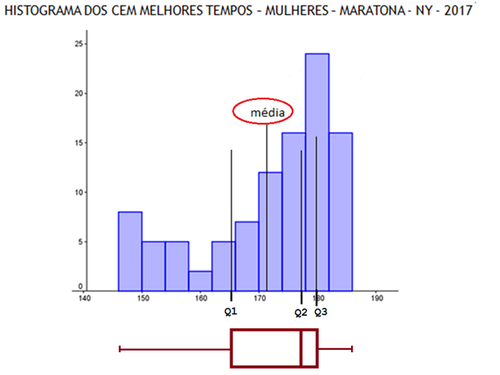
\includegraphics[width=300bp]{box-plot_histograma_mulheres_maratona.png}
\caption{Histograma e boxplot (sem sinalização de valores discrepantes) para os 100 melhores tempos na categoria mulheres}
\label{boxplot-maratona}
\end{figure}

O boxplot é um gráfico muito utlizado em comparações do comportamento de uma variável quantitativa para diferentes categorias, por exemplo, podemos construir boxplots para as categorias mulheres, homens, “cadeira de rodas”{} e “triciclo de mão”{} para identificar diferenças ou semelhanças entre elas.

Veremos adiante como sinalizar valores discrepantes no boxplot. Valores discrepantes em um conjunto de dados são valores que destoam em relação aos demais valores no conjunto. No exemplo cartão de crédito no supermercado (2), o valor $100$ é um valor discrepante em relação aos demais valores do conjunto que variam entre $0$ e $10$.

\subsection{Ramo-e-folhas}

O ramo-e-folhas é uma representação gráfica simples para dados quantitativos. Como cada valor observado é considerado nessa representação, sua construção para conjuntos de dados com mais de $30$ observações é recomendada apenas com o auxílio de tecnologia.

Na construção do ramo-e-folhas sem o auxílio de tecnologia precisamos primeiro conhecer os valores mínimo e máximo para definirmos os ramos e as folhas que são unidades e sub-unidades dos valores observados, respectivamente. Para facilitar, veja o exemplo a seguir.

\begin{example}{Valores consumidos na cantina de uma escola entre 7h e 9h}

Suponha que $20$ pessoas consumiram na cantina de uma escola em um dia no período entre 7 e 9 horas da manhã e que os valores em reais foram registrados: $38, 20, 15, 8, 1, 32, 29, 18, 13, 10, 6, 19, 22, 25, 3, 13, 21, 30, 12 e 25$, nessa ordem.

Observe que os valores registrados variaram entre $1$ real e $38$ reais. Nesse caso, podemos pensar nos ramos como as dezenas 0$, 1, 2 e 3$ e as folhas como as respectivas unidades dessas dezenas. Assim temos a seguinte representação de ramo-e-folhas para esses dados

\begin{figure}[H]
\centering

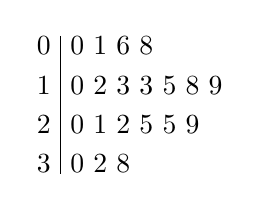
\begin{tikzpicture}[scale=.5]
\draw (0,.25) -- (0,-3.25);
\foreach \x/\y in {0/0{ }1{ }6{ }8,1/0{ }2{ }3{ }3{ }5{ }8{ }9,2/0{ }1{ }2{ }5{ }5{ }9,3/0{ }2{ }8}{
\node [left] at (0,-\x) {\x};
\node [right] at (0,-\x) {\y};
}
\end{tikzpicture}
\end{figure}

Na terceira linha do ramo-e-folhas desse exemplo temos o ramo da dezena $20$. Assim, o número $0$ representado logo a seguir, à direita da barra vertical, corresponde a uma observação de valor $20$, o número 1 em seguida, corresponde a uma observação de valor 21, e assim por diante, de modo que os 20 valores observados ficam organizados de maneira rápida e simples.

Observe que o ramo-e-folhas parece um histograma simplificado com as posições trocadas: classes de valores na escala vertical e frequências na escala horizontal ($4$ observações no primeiro ramo, $7$ observações no segundo ramo, $6$ observações no terceiro ramo e $3$ observações no quarto ramo). As classes correspondem aos intervalos abertos à direita $[0,10[$, $[10,20[$, $[20,30[$ e $[30,40[$.

O ramo-e-folhas pode ser útil na identificação das medidas do esquema dos $5$ números. Tem-se mínimo e máximo $1$ e $38$, respectivamente. O segundo quartil, como temos uma quantidade par de valores é a média dos valores nas posições centrais $10$ e $11$ que são facilmente identificadas no ramo-e-folhas como as observações $18$ e $19$ reais. Assim, o segundo quartil (mediana) é dado por R\$ $18,50$. Para identificarmos os primeiro e terceiro quartis, podemos dividir o conjunto em duas metades de tamanho $10$. Assim o primeiro quartil é dado pela média dos valores nas posições $5$ e $6$ e, o terceiro quartil, pela média dos valores nas posições $15$ e $16$.

\begin{equation*}
Q_1=\frac{10+12}{2}=11\text{ e }  Q_3=\frac{25+25}{2}
\end{equation*}

Resumindo, os cinco números são dados por R\$ 1,00, R\$ 11,00, R\$ 18,50, R\$ 25,00 e R\$ 38,00, Veja na \hyperref[boxplot-cantina]{figura \ref{boxplot-cantina}} o boxplot desses dados, usando a escala dos valores na orientação vertical.

\begin{figure}[H]
\centering

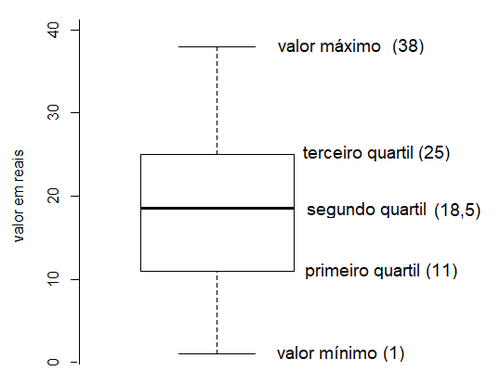
\includegraphics[width=250bp]{boxplotvalores_cantina.png}
\caption{Boxplot dos valores consumidos na cantina}
\label{boxplot-cantina}
\end{figure}

\end{example}
\clearpage
\def\currentcolor{session2}
\begin{objectives}{Categoria homens na maratona}
{
Usar medidas de posição para a comparação das distribuições de uma mesma variável em dois grupos diferentes.
}{1}{2}
\end{objectives}
\begin{sugestions}{Categoria homens na maratona}
{
Nesta atividade serão comparados os dados dos 100 melhores tempos na maratona de Nova Iorque/2017 para as categorias homens e mulheres. A tabela com os 100 melhores tempos em minutos para a categoria homens é fornecida. A comparação será feita com base nas medidas de posição média, quartis, mínimo e máximo, que são fáceis de serem determinadas apesar da quantidade de dados ser 100. No caso da média, a soma dos 100 tempos é informada.
}{1}{2}
\end{sugestions}
\begin{answer}{Categoria homens na maratona}
{
Veja a \hyperref[tabela-maratona-prof]{tabela \ref{tabela-maratona-prof}} com as medidas resumo para as categorias homens e mulheres, correspondendo aos 100 melhores tempos na maratona de Nova Iorque - 2017.



\begin{minipage}{.45\linewidth}
\begin{table}[H]
\centering
\setlength\tabcolsep{2.5pt}
\begin{tabular}{|c|f|f|}
\hline
\tcolor{} & $\tcolor{Mulheres}$ & $\tcolor{Homens}$ \\
\hline
Mínimo & 146{,}88	 & 130{,}88 \\
\hline
Máximo & 185{,}15 & 158{,}33 \\
\hline
Média & 171{,}92 & 150{,}70 \\
\hline
Mediana & 176{,}96 & 153{,}00 \\
\hline
\(Q_1\) & 165{,}87 & 148{,}32 \\
\hline
\(Q_3\) & 179{,}85 & 156{,}62 \\
\hline
\end{tabular}
\caption{Tabela das medidas resumo para as categorias mulheres e homens - Maratona de Nova Iorque/2017}
\label{tabela-maratona-prof}
\end{table}
\end{minipage}
\begin{minipage}{.54\linewidth}
\begin{figure}[H]
\centering

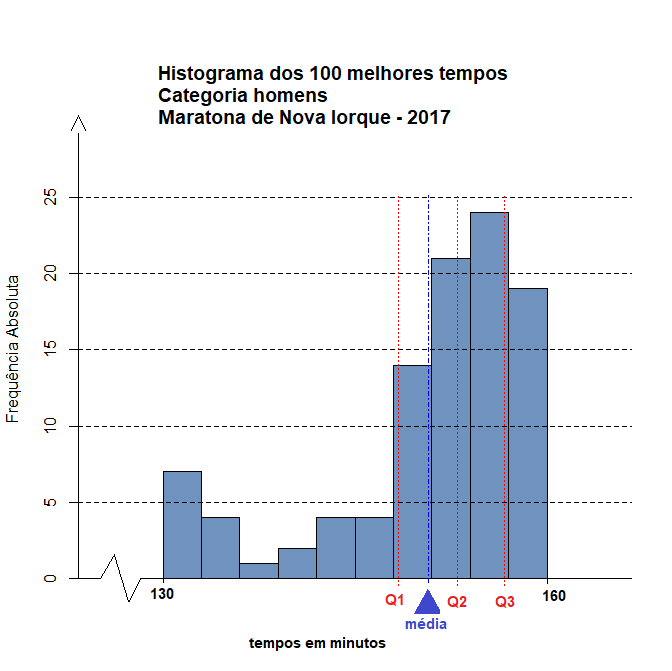
\includegraphics[width=\linewidth]{hist_homens_marcas.png}
\caption{Histograma dos resultados da categoria de Homens da Maratona da Cidade de Nova York do ano 2017, com média, mediana, $Q_1$ e $Q_3$ indicados}
\label{}
\end{figure}
\end{minipage}
}{1}
\end{answer}
\begin{answer}{Categoria homens na maratona}
{
Comparando as duas distribuições (homens e mulheres) é possível perceber que ambas têm a mesma forma com assimetria à esquerda, o que pode ser visualizado pelos histogramas. No entanto, percebe-se que a os homens são mais rápidos (todas as medidas da \hyperref[tabela-maratona-prof]{tabela \ref{tabela-maratona-prof}} são menores para os homens). Além disso, podemos notar que há mais dispersão entre as mulheres, calculando-se a amplitude amostral. Entre as mulheres, a amplitude amostral é $185{,}15-146{,}88=38{,}27$ minutos, enquanto que entre os homens é de $158{,}33-130{,}88=27,45$ minutos. Veja na \hyperref[histograma-comparando]{figura \ref{histograma-comparando}}, dois histogramas correspondentes às categorias homens e mulheres, construídos na mesma escala, ilustrando os comentários da comparação das duas categorias.

\begin{figure}[H]
\centering

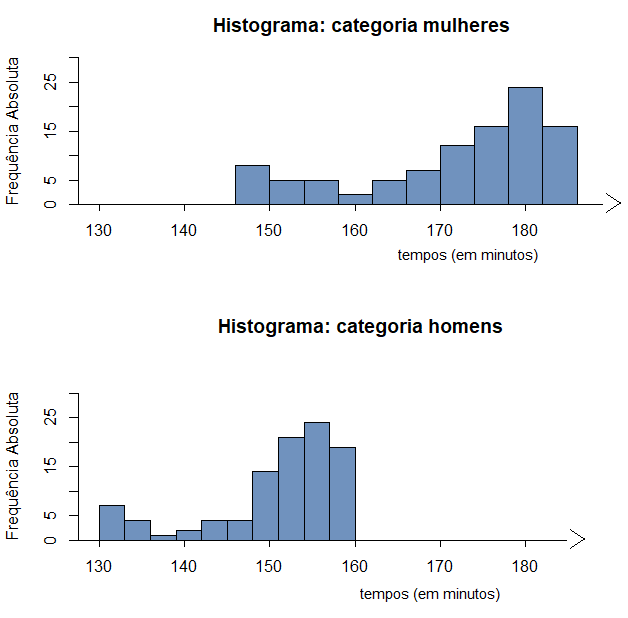
\includegraphics[width=.6\linewidth]{hist_hxm}
\caption{Histogramas dos 100 melhores tempos das categorias homens e mulheres}
\label{histograma-comparando}
\end{figure}

Observe como a comparação entre as duas categorias (homens e mulheres) é mais simples se usarmos a representação dos dados com o \hyperref[boxplot_mulheres_homens]{boxplot}.

\begin{figure}[H]
\centering

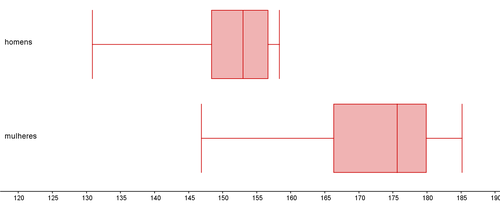
\includegraphics[width=.8\linewidth]{boxplot_mulheres_homens.png}
\caption{Boxplots dos 100 melhores tempos das categorias homens e mulheres (sem sinalização de valores discrepantes)}
\label{boxplot_mulheres_homens}
\end{figure}
}{1}
\end{answer}
\clearmargin
\begin{objectives}{Comparação das diferentes categorias na maratona}
{
\begin{itemize}
\item Comparar distribuições de uma mesma variável para grupos distintos a partir dos histogramas.

\item Perceber a necessidade de usar a mesma escala nos eixos do histograma, para tornar os mesmos comparáveis.
\end{itemize}
}{1}{2}
\end{objectives}
\begin{sugestions}{Comparação das diferentes categorias na maratona}
{
Esta atividade introduz os elementos necessários para a comparação de dois histogramas, a saber: mesmas escalas nos eixos e colunas de frequências relativas.

Os histogramas são apresentados com uma série de perguntas de discussão que podem motivar a formulação do conceito de dispersão de forma intuitiva, que será trabalhado na seguinte seção. Além de mostrar como apenas as medidas de posição não dizem suficiente sobre uma distribuição.

As perguntas não têm respostas fechadas, têm o intuito de gerar uma discussão sobre os assuntos já colocados.
}{1}{2}
\end{sugestions}
\begin{answer}{Comparação das diferentes categorias na maratona}
{
\begin{enumerate}
\item As escalas horizontal e vertical são coincidentes em ambos os histogramas para permitir a comparação. Isto foi discutido no capítulo \hyperref[est1-chap]{\textbf{A Natureza da Estatística}}.
\item Observando-se os histogramas o maior tempo está na categoria de Triciclo de mão.
\item A simples visualização pode remeter a estimativa de 4 horas para estas categorias, valor bem maior do que as médias para homens e mulheres (ativ-maratona-categoria-homens). No entanto, este valor excede muito as médias reais, apresentadas. Isto mostra que estimar o centro de equilíbrio de uma distribuição a partir do histograma não é trivial.
\item Ambos os histogramas apresentam assimetria à direita: grande concentração de dados à esquerda e forma alongada para a direita.
\end{enumerate}
}{1}
\end{answer}
\clearmargin
\begin{answer}{Comparação das diferentes categorias na maratona}
{
\begin{enumerate}\setcounter{enumi}{4}
\item Não é possível, a informação apenas da média é insuficiente para caracterizar a forma do histograma. Outras informações são necessárias para isto.
\item O triciclo de mão apresenta maior dispersão, considerando a amplitude.
\item Na figura a seguir veja uma cosntrução dos boxplots sem sinalização dos valores discrepantes.
\begin{figure}[H]
\centering

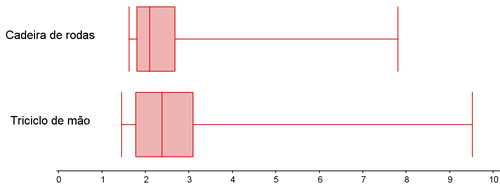
\includegraphics[width=\linewidth]{boxplotcadeiratriciclo_svd.png}
\caption{Boxplots sem sinalização de valores discrepantes para os tempos de chegada em horas das categorias “cadeira de rodas”{} e “triciclo de mão”}
\label{}
\end{figure}
\end{enumerate}
}{1}
\end{answer}

\practice{Medidas de Posição}
\label{\detokenize{PE104-2:sec-praticando1}}\label{\detokenize{PE104-2::doc}}\label{\detokenize{PE104-2:praticando}}\phantomsection\label{\detokenize{PE104-2:ativ-maratona-categoria-homens}}
\begin{task}{ categoria homens na maratona}

Considere os dados da categoria Homens da Maratona da Cidade de Nova Iorque do ano 2017 apresentados na \hyperref[maratona-homens-tabela]{tabela \ref{maratona-homens-tabela}}, já convertidos para minutos.

\begin{table}[H]
\centering
\caption{100 melhores tempos de finalização da Maratona de Nova Iorque 2017 para homens}
\label{maratona-homens-tabela}
\setlength\tabcolsep{4pt}
\begin{tabular}{|c|r|r|r|r|r|r|r|r|r|r|}
\hline
\tcolor{} & \tcolor{+0} & \tcolor{+10} & \tcolor{+20} & \tcolor{+30} & \tcolor{+40} & \tcolor{+50} & \tcolor{+60} & \tcolor{+70} & \tcolor{+80} & \tcolor{+90} \\
\hline
1 & 130,88 & 135,48 & 147,42 & 150,00 & 151,55 & 153,08 & 154,38 & 156,10 & 156,95 & 157,85 \\
\hline
2 & 130,93 & 138,65 & 147,68 & 150,08 & 151,65 & 153,13 & 154,50 & 156,38 & 157,25 & 157,85 \\
\hline
3 & 131,53 & 140,48 & 148,12 & 150,10 & 151,78 & 153,25 & 154,63 & 156,45 & 157,25 & 157,88 \\
\hline
4 & 131,87 & 141,50 & 148,28 & 150,43 & 151,85 & 153,30 & 154,65 & 156,62 & 157,30 & 158,03 \\
\hline
5 & 132,02 & 142,60 & 148,32 & 150,47 & 151,87 & 153,42 & 155,27 & 156,62 & 157,38 & 158,08 \\
\hline
6 & 132,65 & 142,77 & 148,43 & 150,85 & 151,98 & 153,73 & 155,27 & 156,72 & 157,52 & 158,12 \\
\hline
7 & 132,80 & 143,67 & 148,70 & 151,05 & 152,50 & 153,75 & 155,45 & 156,75 & 157,58 & 158,13 \\
\hline
8 & 133,35 & 143,85 & 149,20 & 151,20 & 152,77 & 154,05 & 155,50 & 156,77 & 157,63 & 158,18 \\
\hline
9 & 133,97 & 145,58 & 149,68 & 151,40 & 152,88 & 154,25 & 155,68 & 156,80 & 157,68 & 158,33 \\
\hline
10 & 134,95 & 147,18 & 149,78 & 151,43 & 152,92 & 154,37 & 155,80 & 156,82 & 157,77 & 158,33 \\
\hline
\end{tabular}
\end{table}


Veja na \hyperref[maratona-homens1]{figura \ref{maratona-homens1}}  um histograma destes dados, considerando-se 10 intervalos de classe, a saber, $[130, 133[, [133, 136[, [136,139[, [139,142[, [142,145[, [145,148[,[148,151[, [151,154[, [154, 157[$ e $[157,160[$. As frequências absolutas de cada intervalo de classe estão destacadas no topo dos retãngulos do histograma.


\begin{figure}[H]
\centering

\begin{tikzpicture}[xscale=0.5,yscale=.75, scale=0.35]

\draw (-0.2,0) -- (33.5,0);
\draw (0,0) -- (0,25);

\foreach \x in {0,5,10,15,20,25}  \draw (0,\x) -- (-0.5,\x) node [above, rotate=90] at (-0.3,\x) {\x}  
;


\foreach \x/\y in {3/7,6/4,9/1,12/2,15/4,18/4,21/14,24/21,27/24,30/19}{ \draw [fill=\currentcolor!80] (\x,0) rectangle (\x+3,\y);
\node [above, align=center, scale=.9] at (\x+1.5,\y) {$(\y)$};}

\foreach \x/\y in {3/130,6/\quad,9/136,12/\quad,15/142,18/\quad,21/148,24/\quad,27/153,30/\quad,33/160} \draw (\x,0) -- (\x,-0.25) node [below] {\y};

\foreach \x in {0,5,10,15,20,25}  \draw [dashed] (0,\x) -- (33.5,\x)
;

\node [rotate=90] at (-4,12.5) {frequência absoluta};
\node  at (16.5,-3) {tempos em minutos};
\node [align=center] at (15.6, 27.5) {Histograma dos 100 melhores tempos na categoria \\ Maratona de Nova Iorque - 2017};


\end{tikzpicture}
\caption{Histograma dos resultados da categoria de Homens da Maratona da Cidade de Nova Iorque do ano 2017}
\label{maratona-homens1}
\end{figure}


\begin{enumerate}
\item {} 
Calcule a média dos $100$ melhores tempos na categoria homens, sabendo que a soma dos tempos é dada por $15.069{,}70$ horas.

\item {} 
Calcule a mediana dos 100 melhores tempos na categoria homens.

\item {} 
Identifique o intervalo de classe modal dos 100 melhores tempos na categoria homens.

\item {} 
Determine o primeiro e o terceiro quartis dos 100 melhores tempos na categoria homens.

\item {} 
Localize no histograma a média e os quartis.

\item {} 
Compare com os resultados obtidos para a categoria homens com os obtidos para a categoria mulheres na atividade \hyperref[\detokenize{PE104-0:ativ-maratona-de-ny}]{\textit{A Maratona}} completando a \hyperref[maratona-homens-tabela2]{tabela \ref{maratona-homens-tabela2}}.


\begin{table}[H]
\centering
\caption{Tabela de medidas-resumo para Mulheres e Homens - Maratona de Nova Iorque/2017}
\label{maratona-homens-tabela2}
\begin{tabular}{|c|c|c|}
\hline
\tcolor{} & \tcolor{Mulheres} & \tcolor{Homens} \\
\hline
Mínimo & & \\
\hline
Máximo & & \\
\hline
Média & & \\
\hline
Mediana & & \\
\hline
\(Q_1\) & & \\
\hline
\(Q_3\) & & \\
\hline
\end{tabular}
\end{table}

\item Construa, usando a mesma escala, os boxplots (sem sinalização de valores discrepantes) para as categorias homens e mulheres e destaqie as diferenças encontradas nesse gráfico.
\end{enumerate}

\end{task}

\begin{reflection}

\begin{itemize}
\item {} 
O que seria necessário considerar para poder comparar o histograma da categoria homens com o da categoria mulheres?

\item {} 
Como poderiam ser utilizados os quartis para comparar duas distribuições de dados? Pense em alguma forma de comparar esse dados de forma visual e descreva-a.

\end{itemize}
\end{reflection}

\phantomsection\label{\detokenize{PE104-2:ativ-comparacao-de-diferentes-grupos}}

\needspace{.25\textheight}
\begin{task}{Comparação das diferentes categorias na maratona}

Observe os histogramas da \hyperref[\detokenize{PE104-2:id1}]{figura \ref{\detokenize{PE104-2:id1}}} referentes aos tempos de chegada das categorias “cadeira de rodas”{} e “triciclo de mão”{} na Maratona de Nova Iorque em 2017. Nesse caso, os tempos de chegada foram convertidos para horas e referem-se ao total de participantes que completaram a prova: $51$ na categoria cadeira de rodas e $69$ na categoria triciclo de mão.

\begin{figure}[H]
\centering
\capstart

\noindent\includegraphics[width=300bp]{{Histogramas_cadeira_triciclo}.png}
\caption{Histogramas comparativos das quatro modalidades da maratona de Nova Iorque 2017}\label{\detokenize{PE104-2:id1}}\label{\detokenize{PE104-2:id7}}\end{figure}
\begin{enumerate}
\item {} 
Compare as escalas utilizadas na construção destes histogramas, tanto no eixo horizontal, como no eixo vertical. O que você observou?

\item {} 
Em qual categoria se encontra o atleta que completou a maratona no maior tempo?

\item {} 
Você consegue estimar o tempo médio destas categorias observando os histogramas? Você acha que os tempos médios dessas duas categorias serão muito diferentes dos tempos médios das categorias de homens e de mulheres (atividade \hyperref[\detokenize{PE104-2:ativ-maratona-categoria-homens}]{Categoria Homens na Maratona})?

\item {} 
Observe o quadro a seguir e marque as médias (em horas) nos histogramas. Comente sobre a posição da média em cada caso e sobre a simetria ou assimetria de cada distribuição de dados.

\begin{table}[H]
\centering
\caption{Média das quatro categorias da maratona de Nova Iorque 2017}
\begin{tabular}{|c|c|c|}
\hline
\tcolor{Categoria} & \tcolor{Cadeira de rodas} & \tcolor{Triciclo de mão} \\
\hline
Média & 2,59 & 2,73 \\
\hline
\end{tabular}
\end{table}


\item {} 
Observe que as médias não são muito diferentes. Se você conhecesse apenas a média, seria capaz de perceber a forma destes histogramas? Por quê?

\item {} 
Comparando os dois histogramas, qual distribuição apresenta maior dispersão? Por quê?

\item A partir dos esquemas de cinco números para os tempos de chegada nas categorias cadeira de rodas e triciclo de mão, informados a seguir, construa os respectivos boxplots sem sinalização de valores discrepantes, usando a mesma escala de valores para as duas categorias.

\begin{table}[H]
\centering

\begin{tabular}{|*{6}{c|}}
\hline
\tcolor{Categoria} & \tcolor{Mínimo} & \tmat{$Q_1$} & \tmat{$Q_2$} & \tmat{$Q_3$} & \tcolor{Máximo} \\
\hline
Cadeira de rodas & $1{,}62$ & $1{,}8$ & $2{,}09$ & $2{,}68$ & $7{,}{,}81$ \\
\hline
Triciclo de mão & $1{,}48$ & $1{,}78$ & $2{,}38$ & $3{,}09$ & $9{,}52$ \\
\hline
\end{tabular}
\end{table}

\end{enumerate}
\end{task}

\cleardoublepage
\def\currentcolor{session1}
\begin{objectives}{Estratégia de investimento}
{
Definir medidas que caracterizam a dispersão de um conjunto de dados.
}{1}{1}
\end{objectives}
\begin{sugestions}{Estratégia de investimento}
{
Nessa atividade são apresentados dois conjuntos de dados temporais que apresentam mesma média, mesma mediana e mesma moda e, no entanto, seus gráficos de linha são distintos. O objetivo principal é mostrar que as medidas de posição podem ser insuficientes para caracterizar a distribuição dos dados, levando à necessidade de usar medidas de dispersão. Lembre que é esperado, do Ensino Fundamental, que os estudantes já tenham a noção de amplitude amostral, uma medida bruta de dispersão, pois só leva em conta o mínimo e o máximo observados.

Esta atividade pode ser vinculada às disciplinas de História ou Geografia, por exemplo, no estudo do período da Crise Econômica de 1929 ou outros temas relacionados com o PIB e crescimento econômico.
}{1}{1}
\end{sugestions}
\clearmargin
\begin{answer}{Estratégia de investimento}
{
\begin{enumerate}
\item A escolha pode ser tanto pela $A$ como pela $B$, mas deve vir acompanhada de uma justificativa. Por exemplo, “eu escolheria a companhia A porque os preços oscilam menos”, “escolheria a companhia $B$ porque os preços oscilam mais”, “escolheria a companhia $B$ porque foi a que apresentou maior valor de cotação entre os dias observados”{} etc.

\item Dado que são $10$ observações em cada um dos conjuntos e que as somas das $10$, resultam em $615$, segue que a média das cotações na companhia $A$ é R\$ $61{,}50$, que também é a média das cotações na companhia $B$.

\item Para obter as medianas é necessário antes ordenar os valores. Na tabela a seguir os valores das cotações foram ordenados para cada companhia.


\begin{table}[H]
\centering

\begin{tabular}{|*{11}{f|}}
\hline
\tmat{A} & 56 & 56 & 57 & 58 & 61 & 63 & 63 & 67 & 67 & 67 \\
\hline
\tmat{B} & 33 & 43 & 48 & 52 & 57 & 67 & 67 & 77 & 82 & 90 \\
\hline
\end{tabular}
\end{table}

Como são $10$ observações em cada conjunto e $10$ é um número par, temos que a mediana será dada pela média das duas posições centrais, a saber, posições 5 e 6: Mediana$=\dfrac{x_{(5)}+x_{(6)}}{2}$.

Na companhia $A$ teremos Mediana=$\dfrac{61+63}{2}=62$ reais e, na companhia B, Mediana=$\dfrac{57+67}{2}=62$ reais.

\item Na companhia $A$ o valor mais frequente foi $67$, ocorrendo $3$ vezes. Na companhia $B$, o valor mais frequente foi $67$, ocorrendo duas vezes. Logo, tanto em $A$ como em $B$ o valor da moda foi $67$ reais.

\item Não, pois tais medidas são idênticas nas duas companhias.

\item Analisando os gráficos de linha da figura $57$, percebe-se que as cotações da companhia $B$ variam mais do que as da companhia $A$ e, portanto, como menor risco envolve menos variação, escolheria a companhia $A$. Observe que as amplitudes (diferença entre o maior e menor valores) observadas nas companhias $A$ e $B$ são $67-56=11$ e $90-33=57$, respectivamente, confirmando que na companhia $A$ a variação das cotações é menor.
\end{enumerate}
}{1}
\end{answer}

\explore{Medidas de Dispersão}
\label{\detokenize{PE104-3:explorando-medidas-de-dispersao}}\label{\detokenize{PE104-3::doc}}\label{\detokenize{PE104-3:sec-explorando2}}\phantomsection\label{\detokenize{PE104-3:ativ-estrategia-de-investimento}}

\begin{task}{estratégia de investimento}
Para investir na bolsa de valores compramos ações de empresas por intermédio de uma corretora a um certo preço e depois de um período de tempo vendemos estas ações na expectativa de que seus preços tenham aumentado. No entanto, também podemos perder com o investimento, caso o preço da ação diminua no período de investimento. Uma ação é a menor parte do capital de uma empresa. Veja na figura a seguir um esquema simplificado do investimento na bolsa de valores.

\begin{figure}[H]
\centering

\noindent\includegraphics[width=300bp]{{resized001}.png}
\caption{Esquema simplificado de investimento na bolsa de valores}\label{\detokenize{PE104-3:fig-ativ-bolsa-de-valores}}\label{\detokenize{PE104-3:id1}}\end{figure}

Suponha que você tenha a oportunidade de investir um capital, comprando ações de uma de duas Companhias \(A\) ou \(B\) e para escolher uma das duas, disponha de duas amostras de preços do valor destas ações (em reais) registrados no fechamento da bolsa de valores em dez sextas-feiras consecutivas. Veja na figura e na tabela a seguir a cotação das ações ao longo das últimas 10 semanas.

\begin{figure}[H]
\centering

\begin{tikzpicture}[xscale=1.5,scale=.5, every node/.style={scale=.9}]

\draw [help lines] (0,0) grid (11,7);
\tikzstyle{quad}=[fill=destacado!80,rectangle, minimum height=3pt,minimum width=3pt]
\tikzstyle{los}=[fill=\currentcolor!80,rectangle, minimum height=3pt, minimum width=3pt, rotate=45]

\foreach \x/\y/\z in {1/61/a,2/56/b,3/65/c,4/57/d,5/67/e,6/63/f,7/67/g,8/58/h,9/67/i,10/56/j} \node (\z) [los] at (\x,\y/10-2.5) {};
\draw [very thick, \currentcolor=!80] (a) -- (b) -- (c) -- (d) -- (e) -- (f) -- (g) -- (h) -- (i) -- (j);

\foreach \x/\y/\z in {1/67/A,2/48/B,3/52/C,4/82/D,5/77/E,6/33/F,7/67/G,8/42/H,9/90/I,10/57/J} \node (\z) [quad]  at (\x,\y/10-2.5) {};
\draw [very thick, destacado!80] (A) -- (B) -- (C) -- (D) -- (E) -- (F) -- (G) -- (H) -- (I) -- (J);

\foreach \x in {0,...,11} \node [below] at (\x,-.2) {\x};

\foreach \x/\y in {0/25,1/35,2/45,3/55,4/65,5/75,6/85,7/95} \node [left] at (-.2,\x) {\y};

\node [above,font=\bfseries] at (5.5,7.5) {Cotação das Ações};

\node [below,font=\bfseries] at (5.5,-1) {Semana};
\node [above, rotate=90,font=\bfseries] at (-1,3.5) {Cotação};

\node [los, label=below right:Ações da Companhia A] at (1.5,-2.5) {};

\node [quad, label=right:Ações da Companhia B] at (7,-2.5) {};

\end{tikzpicture}\textbf{}
\caption{Gráficos de linha da cotação das ações}\label{\detokenize{PE104-3:fig-coloque-aqui-o-nome}}\label{\detokenize{PE104-3:id2}}\end{figure}

% \begin{table}[H]
% \centering
% \begin{tabular}{|c|>{$}c<{$}|>{$}c<{$}|}
% \hline
% \tcolor{Semana} & \tmat{A} & \tmat{B} \\
% \hline
% 1 & 61 & 67 \\ 
% \hline
% 2 & 56 & 48 \\
% \hline
% 3 & 63 & 52 \\
% \hline
% 4 & 57 & 82 \\
% \hline
% 5 & 67 & 77 \\
% \hline
% 6 & 63 & 33 \\
% \hline
% 7 & 67 & 67
% \\
% \hline
% 8 & 58 & 42 \\
% \hline
% 9 & 67 & 90 \\
% \hline
% 10 & 56 & 57 \\
% \hline
% Total & 615 & 615 \\
% \hline
% \end{tabular}
% \end{table}

\begin{table}[H]
\centering

\begin{tabular}{|c|*{10}{f|}c|}
\hline
\tcolor{Semana} & 1 & 2 & 3 & 4 & 5 & 6 & 7 & 8 & 9 & 10 & Total \\
\hline
$\tmat{A}$ & 61 & 56 & 63 & 57 & 67 & 63 & 67 & 58 & 67 & 56 & $615$ \\
\hline
$\tmat{B}$ & 67 & 48 & 52 & 82 & 77 & 33 & 67 & 42 & 90 & 57 & $615$ \\
\hline
\end{tabular}
\end{table}

\begin{enumerate}
\item Observando o gráfico, qual das duas companhias você escolheria para investir? Por quê?

\item {} 
Obtenha as médias das cotações das ações das companhias $A$ e $B$ nas semanas observadas e compare-as.

\item {} 
Obtenha as medianas das cotações das ações das companhias $A$ e $B$ nas semanas observadas e compare-as, lembrando que os dados da tabela estão apresentados na ordem temporal.

\item {} 
Obtenha as modas das cotações das ações das companhias $A$ e $B$ nas semanas observadas e compare-as.

\item {} 
Analisando apenas as medidas de posição obtidas em \titem{a)}, \titem{b)} e \titem{c)}, pode-se dizer que as duas companhias diferem uma da outra? Por quê?

\item {} 
Um investimento que apresenta grandes ganhos e perdas pode ser chamado de alto risco, já investimentos cujos valores flutuam pouco são considerados de baixo risco. Se você é um investidor da bolsa de valores avesso ao risco, isto é, você gostaria de escolher o investimento com menores flutuações, em qual das companhias você investiria o seu dinheiro? Por quê?

\end{enumerate}
\end{task}

\arrange{Medidas de Dispersão}
\label{\detokenize{PE104-4:sec-organizando2}}\label{\detokenize{PE104-4::doc}}\label{\detokenize{PE104-4:organizando-as-ideias-medidas-de-dispersao}}

Pela atividade anterior, você deve ter notado que usar apenas medidas de posição para caracterizar uma distribuição não é suficiente. Nos dois conjuntos analisados, vimos que ambos apresentaram média, mediana e moda iguais. No entanto, vimos que um deles apresenta maiores variações de valores do que o outro. A ideia por trás de variação é a noção de dispersão.

Enquanto as medidas de posição procuram resumir o conjunto de dados em alguns valores situados entre dados coletados, as medidas de dispersão buscam avaliar quão dispersos são os dados coletados. Isso é de fundamental importância, pois podemos ter dois conjuntos de dados com as mesmas medidas de posição, como na \hyperref[\detokenize{PE104-3:ativ-estrategia-de-investimento}]{Estratégia de Investimento}, mas com dispersões diferentes, fazendo com que os valores qualitativos dessas medidas de posição sejam também diferentes.

Há uma piada irônica que conta que o Estatístico é o profissional que diz que uma pessoa, ao se sentar numa cadeira com duas placas de metal, uma aquecida a \(100^{\circ}\)C e outra resfriada a \(-40^{\circ}\)C, estará em média confortável, pois temperatura média é de \(30^{\circ}\)C. Na verdade, um Estatístico jamais diria isso, pois ele não toma decisões apenas por uma medida de posição, mas leva em conta também a dispersão dos dados em torno de uma medida de posição. Uma cadeira com duas placas de metal, uma aquecida a \(35^{\circ}\)C e outra a \(25^{\circ}\)C, também tem temperatura média de \(30^{\circ}\)C, mas há menos dispersão da temperatura nessa cadeira que na outra. Assim, embora quantitativamente iguais, os dois valores de \(30^{\circ}\) C não são qualitativamente equivalentes. Há, portanto, que se avaliar a dispersão dos dados coletados, a fim de poder obter conclusões adequadas.

Nesta seção serão apresentadas medidas que buscam caracterizar a dispersão dos dados em um conjunto.

\subsection{Amplitude amostral e distância entre quartis}

Entre as medidas de dispersão mais simples, define-se a amplitude amostral ($R$) como a diferença entre o maior valor e menor valor observados. Usando a notação apresentada anteriormente, dado um conjunto com $n$ observações, temos
\begin{equation*}
\begin{split}\text{Amplitude amostral}=R= \overbrace{x_{(n)}}^{\mathclap{\substack{\text{maior valor} \\ \text{do conjunto}}}}-\underbrace{x_{(1)}}_{\mathclap{\substack{\text{menor valor} \\ \text{do conjunto}}}}\end{split}
\end{equation*}

Uma desvantagem desta medida é que ela considera apenas os dois extremos do conjunto. Ainda é possível que dois conjuntos, tendo mesmas média, moda e mediana, apresentem a mesma amplitude e, no entanto, eles tenham comportamentos diferentes.

\begin{example}{Notas de Matemática}
\phantomsection\label{exemp-notas1}
Considere os seguintes conjuntos de notas de Matemática de duas turmas de reforço, cada uma com 10 alunos.
$$\text{Notas da turma A}=\{ 1,1,1,5,5,5,5,9,9,9\} \text{ e } \text{Notas da turma B}=\{1,3,3,5,5,5,5,7,7,9\}$$

Observe que os dois conjuntos apresentam a mesma média $5$ (a soma das notas é $50$ em ambos), a mesma moda $5$ ($5$ é o valor mais frequente em ambos), a mesma mediana $5$ ($5$ é o valor da posição central em ambos) e a mesma amplitude amostral $8$.

No entanto, comparando os diagramas de pontos correspondentes a cada um deles, ilustrados na \hyperref[\detokenize{PE104-4:fig-diagrama-de-pontos-notas}]{figura \ref{\detokenize{PE104-4:fig-diagrama-de-pontos-notas}}}, é possível perceber diferenças quanto à dispersão das notas em torno da média $5{,}0$ nos dois conjuntos.

\begin{figure}[H]
\centering
\capstart

\resizebox{\linewidth}{!}
{
\begin{tikzpicture}[scale=.7]

\node [above] at (4.5,5) {Turma A};
\draw [<->] (0,4.5) -- (0,0) -- (9.5,0);

\foreach \x in {1,...,9} {
\node [below] at (\x,0) {\x};
\draw (\x,.075) -- (\x,-.075);}

\foreach \x in {1,...,4}{
\node [left] at (0,\x) {\x};
\draw (.075,\x) -- (-.075,\x);}
\node [below left] at (0,0) {0};
\draw (-.1,0) -- (0,0) -- (0,-.1);

\foreach \x/\y in {1/1,1/2,1/3,5/1,5/2,5/3,5/4,9/1,9/2,9/3} \fill [\currentcolor!80] (\x,\y) circle (5pt);
\end{tikzpicture}
\hspace{2em}
\begin{tikzpicture}[scale=.7]

\node [above] at (4.5,5) {Turma B};
\draw [<->] (0,4.5) -- (0,0) -- (9.5,0);

\foreach \x in {1,...,9} {
\node [below] at (\x,0) {\x};
\draw (\x,.075) -- (\x,-.075);}

\foreach \x in {1,...,4}{
\node [left] at (0,\x) {\x};
\draw (.075,\x) -- (-.075,\x);}
\node [below left] at (0,0) {0};
\draw (-.1,0) -- (0,0) -- (0,-.1);

\foreach \x/\y in {1/1,3/1,3/2,5/1,5/2,5/3,5/4,7/1,7/2,9/1} \fill [\currentcolor!80] (\x,\y) circle (5pt);
\end{tikzpicture}
}

\caption{Diagramas de pontos das notas nas turmas A e B}\label{\detokenize{PE104-4:fig-diagrama-de-pontos-notas}}\label{\detokenize{PE104-4:id2}}\end{figure}

Na turma A as notas são mais dispersas em torno da média comparando com a turma B. Mas essa diferença não é captada pela amplitude amostral.
\end{example}


O exemplo \hyperref[exemp-notas1]{\textit{Notas de Matemática}} ilustra a necessidade de uma medida um pouco mais refinada, mas ainda sem considerar todos os valores no conjunto, é a distância entre quartis ($DQ$), definida como a diferença entre o terceiro e primeiro quartis da distribuição. Usando a notação apresentada anteriormente,
\begin{equation*}
\begin{split}DQ=Q_3-Q_s1\end{split}
\end{equation*}

\begin{example}{Notas de Matemática 2}
Vamos retomar os dados do exemplo Notas de Matemática no qual tem-se dois conjuntos de notas, cada conjunto tem 10 observações.
$$\text{Notas da turma A}=\{  1,1,1,5,5,5,5,9,9,9\} \text{ e } \text{Notas da turma B}=\{1,3,3,5,5,5,5,7,7,9\}$$

Podemos dividir os dois conjuntos em duas metades com cinco observações cada e tomar as medianas desses subconjuntos para identificar os primeiro e terceiros quartis das notas.

$$\text{Notas da turma A}=\{\overbrace{1,1,1,5,5}^{\mathclap{\text{primeira metade}}},\underbrace{5,5,9,9,9}_{\mathclap{\text{segunda metade}}}\}$$

Deste modo, temos para a turma \(A\), $Q_1=1$ (mediana da primeira metade) e $Q_3=9$ (mediana da segunda metade) tal que $DQ=9-1=8$ e, para a turma \(B\), usando o mesmo raciocínio, $DQ=7-3=4$, indicando que na turma \(B\), considerando a distância entre quartis, temos menor dispersão, comparada à turma \(A\), observação que pode ser verificada nos diagramas de pontos da  \hyperref[\detokenize{PE104-4:fig-diagrama-de-pontos-notas}]{figura \ref{\detokenize{PE104-4:fig-diagrama-de-pontos-notas}}}.
\end{example}
\needspace{4em}
De fato, a distância entre quartis ($DQ$) também apresenta a desvantagem de somente considerar o primeiro e terceiro quartis, não considerando todas as observações do conjunto. A seguir, serão definidas medidas de dispersão que levam em conta todas as observações realizadas.

\subsection{Boxplot com sinalização de valores discrepantes}

Já vimos como construir o boxplot de um conjunto de dados quantitativos sem a sinalização de valores discrepantes, conhecendo o esquema dos cinco números do conjunto de dados. Agora veremos como é feita a construção do boxplot com essa sinalização.

A distância entre quartis ($DQ=Q_3-Q_1$) é a medida de dispersão utilizada na classificação de valores da distribuição como valores discrepantes, isto é, valores que destoam dos demais no conjunto de dados.

O critério adotado para classificar um valor como discrepante na construção do boxplot é descrito a seguir.

Defina

\begin{equation*}
\text{Cerca inferior}=Q_1-1{,}5\cdot DQ \text{ e Cerca superior} = Q_3+1{,}5\cdot{DQ}
\end{equation*}

Qualquer observação do conjunto de dados que for \textbf{menor do que a cerca inferior ou maior do que a cerca superior} é classificada como valor discrepante e assinalada no boxplot com um asterisco ou algum outro caracter, de acordo com o eixo na escala dos dados.

Na finalização da construção do boxplot, traçam-se segmentos paralelos ao eixo considerado (vertical ou horizontal) partindo dos pontos médios das bases do retângulo e terminando nos maior e menor valores não discrepantes que foram observados.

\begin{example}{Construção do boxplot da atividade 3}

O esquema dos cinco números para a categoria homens dos 100 melhores tempos de chegada (em minutos) é dado por: mínimo$=130{,}88$; $Q_1=148{,}37$; $Q_2=152{,}99$; $Q_3=156{,}66$ e máximo$=158{,}33$.

Portanto, $DQ=Q_3-Q_1=156{,}66-148{,}37=8{,}29$, tal que
\begin{enumerate}
\item $1{,}5\cdot DQ=12{,}435$
\item Cerca inferior$=148{,}37-12{,}435=135{,}935$
\item Cerca superior$=156{,}66+12{,}435=169{,}095$
\end{enumerate}


Como o máximo é $158{,}33$, tem-se que não há valores discrepantes para o lado superior da distribuição. Mas, a cerca inferior é $135{,}935$ minutos, enquanto que o valor mínimo é $130{,}88$ minutos. Nesse caso, será necessário voltar aos dados individuais para poder destacar os valores discrepantes para o lado inferior da distribuição.

Consultando os valores ordenados tem-se que os 12 primeiros tempos de chegada são dados por $130{,}88; 130{,}93; 131{,}53; 131{,}86; 132{,}01; 132{,}65; 132{,}8, 133{,}35; 133{,}96; 134{,}95; 135{,}48$ e $138{,}65$. Logo, concluímos que os $11$ primeiros tempos de chegada na categoria homens são valores discrepantes. Veja na \hyperref[boxplothomens]{figura \ref{boxplothomens}} o boxplot com a sinalização de tais valores.

\begin{figure}[H]
\centering

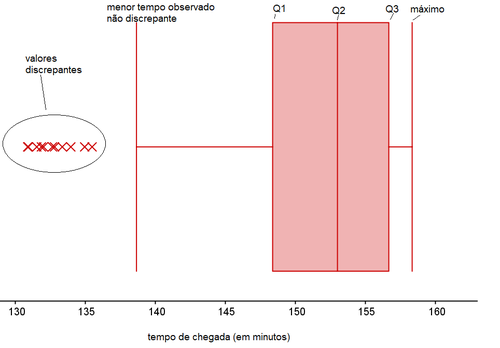
\includegraphics[width=250bp]{boxplothomens.png}
\caption{Boxplot dos 100 primeiros tempos de chegada (em horas) na maratona de Nova York (categoria homens)}
\label{boxplothomens}
\end{figure}
\end{example}

O retângulo do boxplot corresponde aos $50\%$ valores centrais da distribuição, ou seja, metade dos dados estão no intervalo delimitado pela caixa (retângulo) e, a outra metade, está nos dois intervalos delimitados fora da caixa, sendo $25\%$ acima e $25\%$ abaixo da caixa.

As medidas do esquema dos cinco números nos permitem avaliar o grau de assimetria da distribuição. Por exemplo, se

\begin{enumerate}
\item $\text{Mediana}-Q_1\approx Q_3-\text{mediana}$
\item $Q_1-x_{(1)}\approx x_{(n)}-Q_3$
\item $\text{Mediana}-x_{(1)}\approx x_{(n)}-\text{mediana}$
\end{enumerate}
podemos concluir que a distribuição é aproximadamente simétrica, porém se alguns destes pares de intervalos apresentarem comprimentos muito diferentes, isso indica que a distribuição apresenta algum tipo de assimetria. Os pares de intervalos citados são

\begin{enumerate}
\item $[Q_1, \text{mediana}] \text{ e } [\text{mediana}, Q_3]$;
\item $[\text{mínimo}, Q_1] \text{ e } [Q_3, \text{máximo}]$;
\item $[\text{mínimo}, \text{mediana}] \text{ e } [\text{mediana},\text{máximo}]$;
\end{enumerate}

Afinal, para que servem os quartis da distribuição?
\begin{enumerate}
\item identificar valores discrepantes da distribuição (se houver), também conhecidos como valores atípicos ou \textit{outliers};
\item avaliar o grau de assimetria da distribuição empírica do conjunto de dados e
\item construir um gráfico alternativo ao histograma para representar dados quantitativos conhecido como boxplot.
\end{enumerate}

\begin{example}{Construção do bloxplot da atividade 2}
O esquema dos cinco números para a categoria mulheres dos $100$ melhores tempos de chegada (em minutos) é dado por: mínimo=$146,88; Q_1=166,31; Q_2=175,62; Q_3=179,89$ e máximo=$185,15$.

Portanto, $DQ=Q_3-Q_1=179{,}89-166{,}31=13{,}58$, tal que
\begin{enumerate}
\item $1{,}5\cdot DQ=20{,}37$
\item Cerca inferior$=166{,}31-20{,}37=145{,}94$
\item Cerca superior$=179{,}89+20{,}37=200{,}265$
\end{enumerate}

Como o máximo é $185{,}15$, tem-se que não há valores discrepantes para o lado superior da distribuição. O mesmo vale para o lado inferior da distribuição, pois o mínimo é $146{,}88$ e a cerca inferior é $145{,}94$. Logo, na distribuição dos $100$ melhores tempos de chegada na categoria mulheres não existem valores discrepantes.

\begin{figure}[H]
\centering

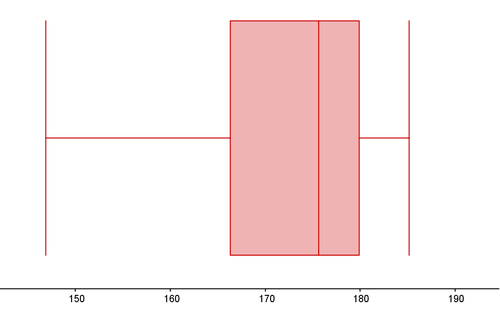
\includegraphics[width=250bp]{boxplotmulheres1.png}
\caption{Boxplot dos 100 primeiros tempos de chegada (em horas) na maratona de Nova York (categoria mulheres)}
\label{boxplotmulheres1}
\end{figure}

Analisando o boxplot da \hyperref[boxplotmulheres1]{figura \ref{boxplotmulheres1}} podemos observar que a distribuição dos $100$ melhores tempos na categoria mulheres apresenta assimetria à esquerda, pois

\begin{enumerate}
\item $Q_2-Q_1>Q_3-Q_2$;
\item $Q_1-\text{valor mínimo}>>\text{valor máximo}-Q_3$;
\item $Q_2-\text{valor mínimo}>>\text{valor máximo}-Q_2$ em que o símbolo $>>$ é usado para representar "bem maior do que".
\end{enumerate}

Podemos concluir o mesmo na categoria homens em que a assimetria à esquerda é mais aparente devido à presença de valores discrepantes à esquerda (lado inferior da distribuição).
\end{example}

\subsection{Desvios da Média}

Considerando o conjunto \(\{ x_1,x_2,\cdots, x_n\}\) com \(n\) observações, seja \(\bar{x}\) a média deste conjunto.  Define-se como um \index{desvio da média}desvio da média, a diferença entre uma observação e a média, a saber,
\begin{equation*}
\begin{split}d_i=x_i-\bar{x}, \quad i=1,2,\cdots n\end{split}
\end{equation*}
Na atividade \hyperref[\detokenize{PE104-3:ativ-estrategia-de-investimento}]{Estratégia de Investimento} os desvios da média, para cada uma das Companhias estão registrados na tabela a seguir.

\begin{table}[H]
\centering
\begin{tabular}{|c|c|c|}
\hline
\tcolor{Semana} & \tcolor{Companhia}\tmat{$A$} & \tcolor{Companhia}\tmat{$B$} \\ 
\hline
1 & -0,5 & 5,5 \\
\hline
2 & -5,5 & -13,5 \\
\hline
3 & 1,5 & -9,5 \\
\hline
4 & -4,5 & 20,5 \\
\hline
5 & 5,5 & 15,5 \\
\hline
6 & 1,5 & -28,5 \\
\hline
7 & 5,5 & 5,5 \\
\hline
8 & -3,5 & -19,5 \\
\hline
9 & 5,5 & 28,5 \\
\hline
10 & -5,5 & -4,5 \\
\hline
Soma & 0 & 0 \\
\hline
\end{tabular}
\end{table}


Poderíamos pensar em usar os desvios da média para definir uma medida de dispersão dos dados em relação à média do conjunto, no entanto, a não ser que todos os valores sejam iguais, teremos valores acima da média e valores abaixo da média de tal modo que os desvios da média poderão apresentar sinais positivos ou negativos. Vimos que a média pode ser interpretada como o centro de massa (ponto de equilíbrio) dos dados e, esta propriedade pode ser descrita da seguinte forma: a soma dos desvios da média de qualquer conjunto de dados é sempre nula.

Com os dados da atividade \hyperref[\detokenize{PE104-3:ativ-estrategia-de-investimento}]{Estratégia de Investimento} você pôde comprovar esta propriedade. Veja na \hyperref[\detokenize{PE104-4:fig-desvios-da-media}]{figura \ref{\detokenize{PE104-4:fig-desvios-da-media}}} a ilustração dos desvios da média das duas companhias na qual a linha pontilhada representa a cotação média da companhia e os segmentos em vermelho indicam o tamanho do desvio da média.

\begin{figure}[H]
\centering
\capstart

\resizebox{\linewidth}{!}
{
\begin{tikzpicture}[scale=.75, every node/.style={scale=.9},xscale=.75]

\draw [help lines] (0,0) rectangle (11,7);
\tikzstyle{quad}=[fill,rectangle, minimum height=3pt,minimum width=3pt]
\tikzstyle{los}=[fill,rectangle, minimum height=3pt, minimum width=3pt, rotate=45]

\tikzstyle{circ}=[fill,circle,inner sep=1.5pt]

\foreach \x/\y/\z in {1/61/a,2/56/b,3/65/c,4/57/d,5/67/e,6/63/f,7/67/g,8/58/h,9/67/i,10/56/j} {
\draw [\currentcolor, very thick] (\x,6.15-2.5) -- (\x,\y/10-2.5);
\node (\z) [circ] at (\x,\y/10-2.5) {};
}

\draw [dashed] (0,6.15-2.5) -- (11,6.15-2.5);


\foreach \x in {2,4,...,10} {\node [below] at (\x,-.2) {\x};
\draw (\x,-.1) -- (\x,.1);}

\foreach \x/\y in {0/30,1/40,2/50,3/60,4/70,5/80,6/90}{
\node [left] at (-.2,\x+.5) {\y};
\draw (-.1,\x+.5) -- (.1,\x+.5);
}

\node [above, scale=1.25] at (5.5,7.5) {Companhia A};

\node [below,font=\bfseries] at (5.5,-.75) {Semana};
\node [above, rotate=90, font=\bfseries] at (-1.5,3.5) {Cotacão};

\end{tikzpicture}
\hspace{2.5em}
\begin{tikzpicture}[scale=.75, every node/.style={scale=.9}, xscale=.75]
\draw [help lines] (0,0) rectangle (11,7);
\tikzstyle{quad}=[fill,rectangle, minimum height=3pt,minimum width=3pt]
\tikzstyle{los}=[fill,rectangle, minimum height=3pt, minimum width=3pt, rotate=45]

\tikzstyle{circ}=[fill,circle,inner sep=1.5pt]

\draw [dashed] (0,6.15-2.5) -- (11,6.15-2.5);


\foreach \x/\y/\z in {1/67/A,2/48/B,3/52/C,4/82/D,5/77/E,6/33/F,7/67/G,8/42/H,9/90/I,10/57/J} {
\draw [\currentcolor!80, very thick] (\x,6.15-2.5) -- (\x,\y/10-2.5);
\node (\z) [circ]  at (\x,\y/10-2.5) {};
}

\foreach \x in {2,4,...,10} {\node [below] at (\x,-.2) {\x};
\draw (\x,-.1) -- (\x,.1);}

\foreach \x/\y in {0/30,1/40,2/50,3/60,4/70,5/80,6/90}{
\node [left] at (-.2,\x+.5) {\y};
\draw (-.1,\x+.5) -- (.1,\x+.5);
}

\node [above, scale=1.25] at (5.5,7.5) {Companhia B};

\node [below, font=\bfseries] at (5.5,-.75) {Semana};
\node [above, rotate=90, font=\bfseries] at (-1.5,3.5) {Cotacão};

\end{tikzpicture}
}
\caption{Desvios da média das cotações nas companhias A e B}\label{\detokenize{PE104-4:fig-desvios-da-media}}\label{\detokenize{PE104-4:id3}}\end{figure}

A {\hyperref[\detokenize{PE104-4:fig-desvios-da-media}]{figura \ref{\detokenize{PE104-4:fig-desvios-da-media}}} reforça a conclusão anterior, da atividade \hyperref[\detokenize{PE104-3:ativ-estrategia-de-investimento}]{Estratégia de Investimento}, de que as cotações da companhia A variam bem menos em torno da média do que as cotações da companhia B.

\needspace{.2\textheight}
Em símbolos, a propriedade de que a soma dos desvios da média é sempre nula, pode ser traduzida em

\begin{equation*}
\displaystyle{\sum^n_{i=1}} d_i=\displaystyle{\sum^n_{i=1}} (x_i-\bar{x})=0,
\end{equation*}

qualquer que seja o conjunto \(\{ x_1,x_2,\cdots, x_n\}\)

Portanto, não será possível usar a soma dos desvios da média como medida de dispersão de um conjunto de dados, pois ela sempre resultará em zero. Isso se deve ao fato de que a soma em valor absoluto dos desvios de sinal negativo é sempre igual a soma dos desvios de sinal positivo, uma consequência da propriedade da média como centro de massa.

Na Companhia $A$ a soma dos desvios negativos é $-19{,}5$ e, dos desvios positivos, $19{,}5$. Na Companhia B a soma dos desvios negativos é $-75{,}5$ e, dos desvios positivos, $75{,}5$.

Uma forma de contornar esta situação, de modo a usar os desvios da média para definir uma medida de dispersão, é eliminar o sinal negativo dos desvios da média de tal forma que a soma nula destes desvios transformados ocorra apenas quando todos os dados são iguais, ou seja, quando qualquer medida de dispersão bem definida deve ser nula.



Veja na seção {\hyperref[\detokenize{PE104-A:sec-para-saber-mais}]{Para saber mais} a demonstração da propriedade de que a soma dos desvios da média é sempre nula.

\subsection{Desvio Médio Absoluto}

Considerando os desvios da média em valor absoluto (\(|x_i-\bar{x}|\)) observe que todos serão não-negativos tal que a soma dos desvios da média em valor absoluto (\(\displaystyle{\sum^n_{i=1}}|x_i-\bar{x}|\)) será nula apenas quando todos os valores do conjunto forem iguais.

Com base na observação anterior, pode-se definir uma medida de dispersão dos dados, considerando todas as observações, chamada desvio médio absoluto ($DM$) que é definida como a média dos desvios da média tomados em valor absoluto.

Na \hyperref[]{tabela} 8.16 são apresentados os desvios da média em valor absoluto das cotações nas companhias $A$ e $B$ e, a respectiva soma.

\begin{table}[H]
\centering
\caption{Desvios da média em valores absolutos para as companhias A e B}
\begin{tabular}{|c|>{$}c<{$}|>{$}c<{$}|}
\hline
\tcolor{Semana} & \tmat{A} & \tmat{B} \\
\hline
1 & 0,5 & 5,5 \\
\hline
2 & 5,5 & 13,5 \\
\hline
3 & 1,5 & 9,5 \\
\hline
4 & 4,5 & 20,5 \\
\hline
5 & 5,5 & 15,5 \\
\hline
6 & 1,5 & 28,5 \\
\hline
7 & 5,5 & 5,5 \\
\hline
8 & 3,5 & 19,5 \\
\hline
9 & 5,5 & 28,5 \\
\hline
10 & 5,5 & 4,5 \\
\hline
Soma & 39,0 & 151,0 \\
\hline
\end{tabular}
\end{table}


Logo, concluímos que o desvio médio absoluto na companhia A é DM= \(\frac{39}{10}=3,9\) reais e, na companhia B, DM= \(\frac{151}{10}=15,1\) reais, indicando que, de fato, a dispersão em torno da média na companhia B é cerca de 4 vezes maior do que na companhia A com relação ao desvio médio (\({15,1}/{3,9}\approx 3,89\)).

De maneira geral, o desvio médio absoluto do conjunto de dados \(\{ x_1,x_2, \cdots, x_n\}\) é
\begin{equation*}
\begin{split}\text{DM} = \frac{1}{n}\cdot \sum^n_{i=1}|x_i-\bar{x}|=\frac{|x_1-\bar{x}|+|x_2-\bar{x}|+\cdots+|x_n-\bar{x}|}{n}\end{split}
\end{equation*}

\subsection{Variância e Desvio Padrão}

Uma outra forma de eliminar o sinal negativo dos desvios da média é elevar ao quadrado cada um deles, tornando-os não-negativos. A variância é definida como uma média dos desvios da média elevados ao quadrado.
\begin{equation*}
\begin{split}\text{variância} = \frac{1}{n}\cdot \sum^n_{i=1} (x_i-\bar{x})^2=\frac{(x_1-\bar{x})^2+(x_2-\bar{x})^2+\cdots+(x_n-\bar{x})^2}{n}\end{split}
\end{equation*}
Na \hyperref[desvios-da-media]{tabela \ref{desvios-da-media}} são apresentados os desvios da média elevados ao quadrado das cotações nas companhias A e B e, a respectiva soma.

\begin{table}[H]
\centering
\caption{Desvios da média elevados ao quadrado para as companhias A e B}
\label{desvios-da-media}
\begin{tabular}{|c|>{$}c<{$}|>{$}c<{$}|}
\hline
\tcolor{Semana} & \tmat{A} & \tmat{B} \\
\hline
1 & 0,25 & 30,25 \\
\hline
2 & 30,25 & 182,25 \\
\hline
3 & 2,25 & 90,25 \\
\hline
4 & 20,25 & 420,25 \\
\hline
5 & 30,25 & 240,25 \\
\hline
6 & 2,25 & 812,25 \\
\hline
7 & 30,25 & 30,25 \\
\hline
8 & 12,25 & 380,25 \\
\hline
9 & 30,25 & 812,25 \\
\hline
10 & 30,25 & 20,25 \\
\hline
Soma & 188,5 & 3018,5 \\
\hline
\end{tabular}
\end{table}

Logo, concluímos que a variância na companhia A é \(\dfrac{188,5}{10}=18,85\text{ reais}^2\) e, na companhia B, \(\dfrac{3018,5}{10}=301,85\text{ reais}^2\) , indicando que a dispersão em torno da média na companhia B é cerca de 16 vezes maior do que na companhia A com relação à variância  (\(301,85/18,85\approx 16\)).

Quando lidamos com grande quantidade de dados, calcular a variância usando a definição apresentada será uma tarefa maçante, pois após calcular a média de muitos dados, teremos que calcular cada desvio da média, elevá-los ao quadrado e, finalmente, somá-los. Para conjuntos de dados com mais de $10$ elementos será, em geral, muito trabalhoso calcular a variância desta forma. Um modo mais simples para calcular a variância é apresentado a seguir. Pode-se mostrar que o numerador da fórmulada variância é dado por


\begin{equation*}
\begin{split}\sum^n_{i=1} (x_i-\bar{x})^2 = \sum^n_{i=1} x^2_i-n\cdot \bar{x}^2\end{split}
\end{equation*}
Assim, basta conhecer a soma simples (\(\displaystyle{\sum^n_{i=1}}x_i\)), para determinar a média \(\bar{x}\), e a soma de quadrados (\(\displaystyle{\sum^n_{i=1}}x^2_i\)) para calcular a variância.

A demonstração desta igualdade está na Seção {\hyperref[\detokenize{PE104-A:sec-para-saber-mais}]{Para saber mais}.

Na atividade \hyperref[\detokenize{PE104-3:ativ-estrategia-de-investimento}]{Estratégia de Investimento} , podemos verificar que na companhia $A$, \(\bar{x}=61,5\) e \(\displaystyle{\sum^{10}_{i=1}} x^2_i=38.011\) tal que a variância em A pode ser calculada por
\begin{equation*}
\begin{split}\text{variância}=\frac{1}{10}\cdot (38.011-10\cdot 61,5^2)=18,85\text{ reais}^2\end{split}
\end{equation*}
e, na companhia B,

\(\bar{x}=61,5\) e \(\displaystyle{\sum^{10}_{i=1}} x^2_i=40.841\) tal que a variância em B pode ser calculada por
\begin{equation*}
\begin{split}\text{variância}=\frac{1}{10}\cdot (40.841-10\cdot 61,5^2)=301,85\text{ reais}^2\end{split}
\end{equation*}
Vimos que o desvio médio absoluto da companhia B foi aproximadamente 4 vezes maior do que o da companhia A. Na comparação de variâncias, a variância da companhia B foi cerca de 16 vezes maior do que a da companhia A. Este grande aumento deve-se ao fato de que consideramos os desvios da média elevados ao quadrado no cálculo da variância. Observe que a unidade de medida na variância é o quadrado da unidade de medida das observações. Para retornar à escala de medida das observações, basta extrair a raiz quadrada da variância, levando a definição de desvio padrão, uma medida de dispersão em torno da média, na mesma unidade das observações.
\begin{equation*}
\begin{split}\text{desvio padrão}=\sqrt{\text{variância}}\end{split}
\end{equation*}
No exemplo das cotações, podemos verificar que na companhia $A$,
\begin{equation*}
\begin{split}\text{desvio padrão}=\sqrt{18,85} \approx 4,34 \text{ reais}\end{split}
\end{equation*}
e, na companhia $B$,
\begin{equation*}
\begin{split}\text{desvio padrão}=\sqrt{301,85}\approx 17,37\text{ reais}\end{split}
\end{equation*}
Verifique que o desvio padrão da companhia B é aproximadamente 4 vezes maior do que o da companhia A.

\begin{observation}{Por que o desvio padrão é preferível ao desvio médio?}

Você deve estar se perguntando por que se utiliza o desvio padrão na Estatística em detrimento do desvio médio, cujo cálculo é bem mais simples. A resposta é um tanto complexa para o nível em que estamos, mas ela está associada à necessidade na Estatística de se minimizar estruturas de maneira simples. O desvio médio faz uso da função modular \(f(x)=|x|\), que não possui boas propriedades matemáticas para a minimização, por possuir na sua forma uma mudança abrupta em torno de \(x=0\),  enquanto que a variância faz uso da função quadrática \(f(x)=x^2\), representando parábolas de vértice suave e cujas propriedades analíticas são bem conhecidas. Veja a \hyperref[\detokenize{PE104-4:fig-coloque-aqui-o-nome}]{figura \ref{\detokenize{PE104-4:fig-coloque-aqui-o-nome}}}.

\begin{figure}[H]
\centering
\capstart

\begin{tikzpicture}[every node/.style={scale=.75}]

\draw [->] (-4.5,0) -- (4.5,0);
\draw [->] (0,-1.5) -- (0,4.3);

\draw [domain=-2:2, \currentcolor, thick] plot (\x,{(\x)^2}) node [left, shift={(-.3,-.5)}] {$f(x)=x^2$};
\draw [domain=0:4, destacado, thick] plot (\x,{\x}) node [below right, shift={(-.5,-.5)}] {$f(x)=|x|$};
\draw [domain=-4:0, destacado, thick] plot (\x,{-\x});

\foreach \x in {-4,...,-1,1,2,...,4} {
\draw (\x,-.075) -- (\x,0.075);
\node [below] at (\x,-0.075){\x};}

\foreach \x in {-1,1,2,...,4} {
\draw (-.075,\x) -- (.075,\x);
\node [left] at (-.075,\x) {\x};}

\node [below left] at (-.075,-.075) {0};

\node [align=justify, \currentcolor, font=\bfseries] at (-2.5,-1) {Observe mundança suave de \\ comportamento em torno de \\ $x=0$ na função quadrática};

\node [align=justify, destacado, font=\bfseries] at (2.5,-1) {Observe mundança abrupta de \\ comportamento em torno de \\ $x=0$ na função módulo};
\end{tikzpicture}

\caption{Funções modular e quadrática com destaque para o comportamento em torno de $x=0$.}\label{\detokenize{PE104-4:fig-coloque-aqui-o-nome}}\label{\detokenize{PE104-4:id6}}\end{figure}

Muitos problemas de estimação de posição de astros na Física são resolvidos por funções quadráticas por esse motivo, um legado deixado pelo matemático alemão Carl Friedrich Gauss (1777 - 1855) no chamado  \href{https://pt.wikipedia.org/wiki/M\%C3\%A9todo\_dos\_m\%C3\%ADnimos\_quadrados}{Método dos Mínimos Quadrados}.

\begin{figure}[H]
\centering
\capstart

\noindent\includegraphics[width=100bp]{{gauss}.png}
\caption{Carl Friedrich Gauss}\label{\detokenize{PE104-4:id1}}\label{\detokenize{PE104-4:id7}}\end{figure}
\end{observation}

\subsection{Variância populacional e amostral, desvio padrão populacional e amostral}

No capítulo \textbf{\hyperref[est1-chap]{A Natureza Estatística}} foram apresentados os conceitos parâmetro e estimador. Parâmetro é uma característica numérica da população, em geral desconhecida; enquanto estimador é uma função dos dados da amostra (subconjunto da população), usada para estimar o parâmetro. Em geral, usam-se letras gregas para denotar parâmetros.


Se dispomos de uma amostra da população, de fato, calculamos a média amostral e a variância amostral (funções dos dados da amostra) e usamos estes resultados como estimativas da média populacional e da variância populacional. Como já foi comentado anteriormente, a média amostral tem boas propriedades como estimador da média populacional. No entanto, é possível mostrar que a variância calculada pela fórmula apresentada no início deste capítulo é um estimador que tende a produzir valores menores do que o valor da variância da população. Dizemos que é um estimador viesado por essa razão.

Para contornar este defeito do estimador, usamos o denominador \(n-1\) no lugar de \(n\). Observe que com isto os valores produzidos serão um pouco maiores, pois o denominador é um pouco menor.

Assim, as expressões que deverão ser usadas quando o conjunto de dados sob estudo é uma amostra da população são dadas por
\begin{align*}\!\begin{aligned}
\text{variância amostral}=s^2=\frac{1}{n-1}\sum^n_{i=1}(x_i-\bar{x})^2\\
\text{desvio padrão amostral}=\sqrt{s^2}=s\\
\end{aligned}\end{align*}
Na maioria das vezes trabalhamos com amostras. Assim, neste capítulo, salvo menção em contrário, estaremos sempre calculando a variância amostral (\(s^2\)) e o desvio padrão amostral (\(s\)), mesmo que o termo “amostral”{} esteja omitido.

Se você estiver trabalhando com uma amostra e usar o denominador \(n\) para calcular a variância, isso implicará que você escolheu um estimador viesado, pois tende a produzir estimativas que são menores do que o verdadeiro valor da variância. Observe que se você estiver trabalhando com amostras muito grandes, essa diferença não será importante, pois haverá pouca diferença entre dividir por \(n\) ou por \(n-1\).

Expressões que deverão ser consideradas quando o conjunto de dados sob estudo refere-se à população com \(N\) elementos:
\begin{align*}\!\begin{aligned}
\text{variância populacional} = \sigma^2=\frac{1}{N}\sum^n_{i=1}(x_i-\mu)^2\\
\text{desvio padrão populacional}=\sqrt{\sigma^2}=\sigma\\
\end{aligned}\end{align*}
em que \(\mu\) representa a média populacional.


\needspace{.25\textheight}
\begin{example}{Variância populacional versus variância amostral}
Para ilustrar a discussão anterior suponha uma população com apenas 4 elementos, caracterizada pelo conjunto de valores ${1,2,3,4}$.

Nesse caso, temos todas as informações sobre a população. Observe que

\begin{enumerate}
\item o tamanho da população é $N=4$,
a média da populacional é dada por $\mu=\dfrac{1+2+3+4}{4}=2,5$ e
a variância populacional é dada por $\sigma^2=\dfrac{(1-2{,}5)^2+(2-2{,}5)^2+(3-2{,}5)^2+(4-2{,}5)^2}{4}=1{,}25$.
\end{enumerate}

Suponha que iremos trabalhar com amostras de tamanho $n=2$ dessa população. Usando amostragem aleatória simples (sorteios com reposição dos elementos da população), observe que existem ao todo $16$ amostras possíveis. Para cada amostra possível, vamos calcular a média da amostra e a variância da amostra, considerando os denominadores $n--$ e $n$. Veja os resultados na tabela 8.19.

\begin{table}[H]
\centering

\begin{tabular}{|*{5}{>{$}c<{$}|}}
\hline
$\tcolor{Amostra}$ & $\tcolor{Valores}$ & $\tcolor{Média amostral}$ & \tmat{s^2(n-1)} & \tmat{\sigma^2(n)} \\
\hline
1 & 1 \text{ e } 1 & 1 & 0 & 0 \\
\hline
2 & 1 \text{ e } 2 & 1{,}5 & 0{,}5 & 0{,}25 \\
\hline
3 &	1 \text{ e } 3 & 2 & 2 & 1 \\
\hline
4 & 1 \text{ e } 4 & 2{,}5 & 4{,}5 & 2{,}25 \\
\hline
5 & 2 \text{ e } 1 & 1{,}5 & 0{,}5 & 0{,}25 \\
\hline
6 & 2 \text{ e } 2 & 2 & 0 & 0 \\
\hline
7 & 2 \text{ e } 3 & 2{,}5 & 0{,}5 & 0{,}25 \\
\hline
8 & 2 \text{ e } 4 & 3 & 2 & 1 \\
\hline
9 & 3 \text{ e } 1 & 2 & 2 & 1 \\
\hline
10 & 3 \text{ e } 2 & 2{,}5 & 0{,}5 & 0{,}25 \\
\hline
11 & 3 \text{ e } 3 & 3 & 0 & 0 \\
\hline
12 & 3 \text{ e } 4 & 3{,}5 & 0{,}5 & 0{,}25 \\
\hline
13 & 4 \text{ e } 1 & 2,5 & 4,5 & 2,25 \\
\hline
14 & 4 \text{ e } 2 & 3 & 2 & 1 \\
\hline
15 & 4 \text{ e } 3 & 3{,}5 & 0{,}5 & 0{,}25 \\
\hline
16 & 4 \text{ e } 4 & 4 & 0 & 1 \\
\hline
 & $soma$ & 40 & 20   & 11 \\
\hline
\end{tabular}
\end{table}

\end{example}


\needspace{.25\textheight}
\clearmargin
\clearmargin
\begin{objectives}{Inflação anual}
{
\begin{itemize}
\item Comparar diferentes conjuntos de dados que apresentam a mesma variância, mas suas médias são diferentes.

\item Perceber a necessidade de definir uma medida que avalie a magnitude da variância (desvio padrão) em relação à média.
\end{itemize}
}{1}{1}
\end{objectives}
\begin{sugestions}{Inflação anual}
{
Nesta atividade são apresentados dois conjuntos de dados cujas variâncias são iguais, mas cujas médias são distintas. Pretende-se na discussão, levar à definição de coeficiente de variação, uma medida útil para avaliar a magnitude da variância. Como o dado observado é a inflação anual de um país, a atividade começa com um pequeno texto introdutório sobre inflação.
}{1}{1}
\end{sugestions}
\begin{answer}{Inflação anual}
{
\begin{enumerate}
\item No país $A$, a inflação média anual, considerando estes 5 anos, é $\bar{x}=\frac{10}{5}=2{,}00\%$. No país $B$, a inflação média anual, considerando estes 5 anos, é $\bar{x}=0{,}055=0{,}01\%$. Logo, as inflações anuais médias dos dois países são bem diferentes.

\item Usando a fórmula simplificada para o cálculo da variância, temos, para o país $A$, $s^2=\frac{1}{5-1}(20,1-5\cdot2^2)=0{,}025(\%^2)$. Para o país $B$, temos $s^2=\frac{1}{5-1}(0{,}1005-5\cdot0{,}012)=0{,}025(\%^2)$. Logo, as variâncias destes dois conjuntos de inflações anuais são iguais e, consequentemente, os desvios padrões também são iguais.

\item Verifique que os cinco desvios da média produzidos pelos dados dos dois países são idênticos, levando à mesma variância (mesmo desvio padrão). No entanto, a média no país $A$ ($2\%$) é bem maior do que no país $B$, indicando uma variação relativa à média menos forte do que no país $B$. A seguir, será definido o coeficiente de variação, que avalia essa propriedade de dispersão relativa à média. Observe que o desvio padrão para os dois países é $\sqrt{0{,}025}\approx0{,}16\%$ de modo que no país A o desvio padrão corresponde a $8\%$ da média $(\frac{0{,}16}{2}=0{,}08)$, enquanto que no país B, corresponde a $1.600\%$ da média $(\frac{0{,}16}{0{,}01}=16)$, ou seja, a flutuação em torno da média é muito mais forte no país $B$.
\end{enumerate}
}{1}
\end{answer}
\begin{example}{Medidas de posição e dispersão usando o GeoGebra}
Podemos usar o GeoGebra para calcular várias das medidas trabalhadas nesse capítulo, bem como para construir boxplots e histogramas. Considere o conjunto das Notas de Artes sem bonificação da primeira atividade do capítulo. São 35 notas que podem ser inseridas na planilha do GeoGebra, conforme \hyperref[GeoG1]{figura \ref{GeoG1}}. Lembre-se que o GeoGebra adota o ponto como separador decimal.

\begin{figure}[H]
\centering

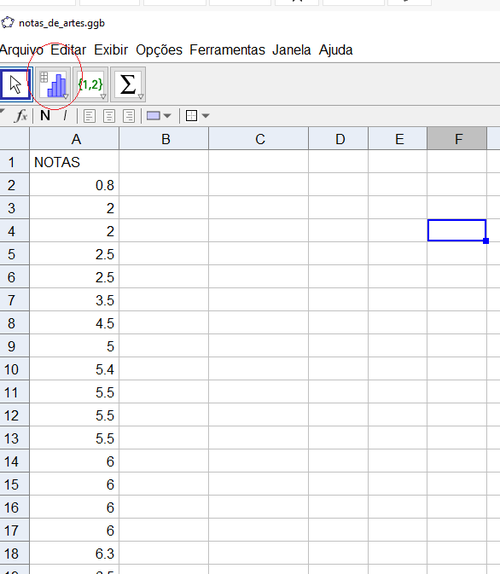
\includegraphics[width=300bp]{GeoG1.png}
\caption{Tela de planilha do GeoGebra com as notas de artes, destacando o botão com imagem de um histograma}
\label{GeoG1}
\end{figure}

Para calcular as medidas ou mesmo construir gráficos desse conjunto de dados, basta selecionar a coluna com os dados e clicar no botão cuja imagem é um histograma. Veja a \hyperref[GeoG2]{figura \ref{GeoG2}}.

\begin{figure}[H]
\centering

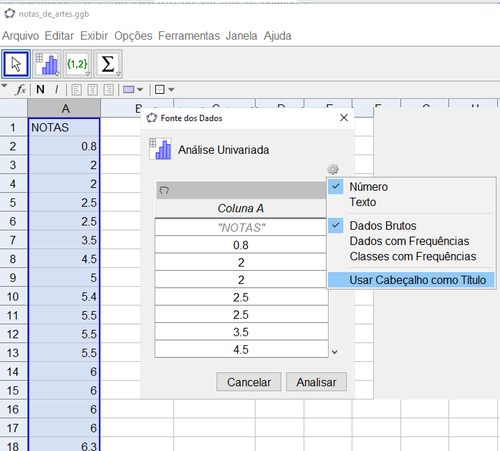
\includegraphics[width=275bp]{GeoG2.png}
\caption{Tela de planilha do GeoGebra com as notas de artes, destacando a opção análise univariada}
\label{GeoG2}
\end{figure}

\begin{figure}[H]
\centering

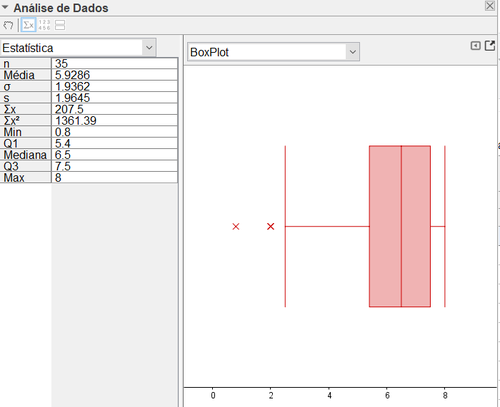
\includegraphics[width=275bp]{GeoG3.png}
\caption{Medidas resumo e boxplot do conjunto de notas de Artes usando o GeoGebra}
\label{GeoG3}
\end{figure}

A \hyperref[GeoG3]{figura \ref{GeoG3}} mostra a saída do GeoGebra da análise univariada das notas de artes com a construção do respectivo boxplot.

\begin{enumerate}
\item $n$ -- número de observações consideradas,
\item média -- média aritmética,
\item $\sigma$ -- desvio padrão obtido a partir do cálculo da variância considerando o denominador $n$, recomendado quando o conjunto representa a população e não uma amostra da população,
\item $s$ -- desvio padrão amostral calculado a partir da variância amostral usando denominador $n-1$,
\item $\sum x$ -- soma simples dos valores de um conjunto,
\item $\sum x^2$ -- soma de quadrados dos valores do conjunto,
\item Min, $Q_1$, Mediana $Q_3$ e Max: medidas do esquema dos cinco números, a saber, mínimo, primeiro, segundo e terceiro quartis e máximo.
\end{enumerate}
\end{example}


\begin{task}{inflação anual}
\label{inflacao-dois-paises}

A seguir são apresentados dados sobre as inflações anuais em dois países. Antes de trabalhar com os dados, vamos tentar explicar o que é \index{inflação}inflação. De uma maneira bem simples, pode-se dizer que a inflação é o aumento contínuo nos preços de produtos e serviços. Esse aumento costuma ser avaliado de forma mensal, gerando os índices de inflação, que refletem a variação nos preços.

A inflação pode ser medida de várias formas. O índice oficial de inflação no Brasil é o IPCA (Índice de Preços ao Consumidor Amplo), que mede a variação mensal de preços de produtos considerando o consumo de famílias com renda mensal entre 1 e 40 salários mínimos. O IBGE (Instituto Brasileiro de Geografia e Estatística) é o orgão responsável pela medição e divulgação do IPCA. Veja neste
\href{https://www.youtube.com/watch?v=JVcDZOlIMBk}{link}, um vídeo produzido pelo IBGE, explicando o IPCA.

Foram observadas as inflações anuais de dois países $A$ e $B$ para os anos de 2011 a 2015, conforme tabela a seguir.

\begin{table}[H]
\centering
\caption{Inflação anual}
\begin{tabular}{|c|c|c|c|c|c|c|}
\hline
\tcolor{País} & \tcolor{2011} & \tcolor{2012} & \tcolor{2013} & \tcolor{2014} & \tcolor{2015} & \tcolor{Soma} \\
\hline
$A$ & $2{,}00\%$ & $1{,}80\%$ & $2{,}10\%$ & $2{,}20\%$ & $1{,}90\%$ & $10{,}00\%$ \\
\hline
$B$ & $0{,}01$\% & $-0{,}19\%$ & $-0{,}09\%$ & $0{,}21\%$ & $0{,}11\%$ & $0{,},05\%$ \\
\hline
\end{tabular}
\end{table}

\begin{enumerate}
\item {} 
Calcule as médias das inflações anuais dos dois países. Há diferenças entre elas?

\item {} 
Calcule as variâncias das inflações anuais dos dois países, sabendo que para o país $A$, \(\displaystyle{\sum^5_{i=1}}x^2_i=20,1\)  (\% \(^2\) ) e para o país $B$,  \(\displaystyle{\sum^5_{i=1}}x^2_i=0,1005\)  (\% \(^2\) ). Há diferença entre elas?

\item {} 
Qual dos países apresenta maior variação inflacionária quando comparada à média inflacionária?

\end{enumerate}
\end{task}


\subsection{Coeficiente de variação}

Nem sempre uma variância pequena (e consequentemente desvio-padrão pequeno) significa pouca dispersão. Tampouco uma variância grande é sempre indicador de alta dispersão. Esses valores podem ser altos ou baixos devido à magnitude (ordem de grandeza) dos dados observados. Se medimos observações em microscópio, por exemplo, teremos inevitavelmente valor numericamente baixo de variância, podendo no entanto haver alta dispersão dos dados no nível microscópico. Da mesma maneira, ao medir os produtos internos brutos brasileiros em dólares em vários anos teremos valores observados de alta magnitude, gerando variância numericamente grande, mas não necessariamente indicando alta dispersão.

Na atividade \hyperref[inflacao-dois-paises]{Inflação anual}, estudamos dois conjuntos de dados que apresentam médias diferentes, mas variâncias iguais. Podemos dizer que o impacto da variância em relação à média é o mesmo para os dois conjuntos? Comparando o valor do desvio padrão de cerca de $0{,}16\%$ à média do país $A$ de $2\%$, vemos que ele é pequeno em relação à média. Comparando o valor do desvio padrão $0{,}16\%$ em relação à média do país B de $0{,}01\%$, vemos que ele é muito grande em relação à média. Neste caso dizemos que no país $A$ os dados apresentam variação relativa em torno da média pequena. Já, no país $B$, os dados apresentam variação relativa em torno da média grande.



O \index{coeficiente de variação}coeficiente de variação é uma medida usada para calcular a variação relativa dos dados de um conjunto em torno da média: quanto maior seu valor, maior é a variação relativa em torno da média.
\begin{description}
\item[{Coeficiente de variação\index{Coeficiente de variação|textbf}}] \leavevmode\phantomsection\label{\detokenize{PE104-4:term-coeficiente-de-variacao}}
é a razão entre o desvio padrão e a média. Em geral, ele é descrito em termos percentuais.

\end{description}

O coeficiente de variação amostral, em termos percentuais, é calculado  por
\begin{equation*}
\begin{split}CVA=\frac{s}{\bar{x}}\cdot 100 \%\end{split}
\end{equation*}
em que \(s\) é o desvio padrão amostral e \(\bar{x}\) é a média amostral.

Esta expressão é usada quando dispomos de uma amostra da população. Se, dispomos dos dados da população, então o coeficiente de variação populacional é dado por
\begin{equation*}
\begin{split}CVP=\frac{{\sigma}}{\mu}\cdot 100\%\end{split}
\end{equation*}
em que \(\sigma\) é o desvio padrão populacional e \(\mu\) é a média populacional.

Observe que o coeficiente de variação só é definido para conjuntos cuja média é diferente de zero.

Uma regra empírica para avaliar frequências de valores em intervalos em torno da média que pode ser útil, é obtida a partir das propriedades de um modelo teórico conhecido como densidade normal de probabilidades. Entre várias propriedades desta densidade, destaca-se que ela é simétrica e unimodal tal que média, mediana e moda são iguais. Veja na \hyperref[\detokenize{PE104-6:fig-densidade-normal}]{figura \ref{\detokenize{PE104-6:fig-densidade-normal}}} 8.39 uma ilustração da densidade normal com média \(\mu\) e desvio padrão \(\sigma\), também conhecida como a curva em forma de sino.
\clearpage
{\def\currentcolor{session2}
\begin{objectives}{Comparação de conjuntos de dados}
{
Comparar diferentes distribuições de uma mesma variável quando separada por grupos.


}{1}{1}
\end{objectives}
\begin{sugestions}{Comparação de conjuntos de dados}
{
Nesta atividade serão coletados dados de uma mesma variável que possa ser separada em grupos, com o intuito de comparar as suas medidas de posição e dispersão. Sugerem-se algumas opções, dependendo do tamanho da turma e do contexto escolar, podem até ser escolhidas variáveis distintas para grupos pequenos de alunos, por exemplo, um grupo trabalha com as médias de Matemática, outro grupo trabalha com alturas, etc.

Uma vez coletados os dados, serão calculadas suas medidas de posição e dispersão e comparadas, tentando orientar os estudantes a comentar as observações e não apenas fazer os cálculos. Para a realização dos cálculos deve ser usado suporte tecnológico: calculadoras, aplicativos, etc.

O intuito é dar uma perspectiva para os estudantes da forma em que a estatística é utilizada na ciência para responder perguntas como:

\begin{itemize}
\item Uma determinada espécie vegetal cresce melhor perto de uma fonte de água ou longe da mesmo? Na sombra de uma árvore ou recebendo luz direta do sol?
\item As meninas são mais altas que os meninos numa certa idade? Acontece o mesmo em todas as idades?
\end{itemize}

De forma ideal, pode ser formulada primeiro a pergunta, e depois coletados os dados, apelando a informações encontradas num artigo científico ou numa publicação de jornal, com o intuito de tentar contrastar uma afirmação dada num texto com dados coletados diretamente.
}{1}{1}
\end{sugestions}
\clearmargin

}
\begin{figure}[H]
\centering
\capstart

\noindent\includegraphics[width=300bp]{{densidadenormal_1}.png}
\caption{Densidade Normal com região colorida no intervalo entre \(\mu-\sigma\) e \(\mu+\sigma\) , cuja área corresponde a aproximadamente 0,67 da área total igual a 1.}\label{\detokenize{PE104-6:fig-densidade-normal}}\label{\detokenize{PE104-6:id8}}\end{figure}

A regra empírica estabelece que em distribuições aproximadamente simétricas para as quais são raros ou mesmo não exitem valores discrepantes,
\begin{enumerate}
\item {} 
a frequência relativa de valores no intervalo \([\bar{x}-s;\bar{x}+s]\) é aproximadamente $67\%$,

\item {} 
a frequência relativa de valores no intervalo \([\bar{x}-2\cdot s; \bar{x}+2\cdot s]\) é aproximadamente $95\%$.

\end{enumerate}

No caso dos dados da atividade \hyperref[\detokenize{PE104-0:ativ-maratona-de-ny}]{A Maratona} vimos que não existem valores discrepantes na categoria mulheres, mas a distribuição apresenta assimetria à esquerda. Ainda assim, contando frequência de observações que nos intervalos definidos por \([\bar{x}-s;\bar{x}+s]\) e  \([\bar{x}-2\cdot s; \bar{x}+2\cdot s]\),  obtém-se $69\%$ e $93\%$, respectivamente. Observe que este valores estão próximos dos valores estipulados pela regra empírica, mesmo com este conjunto apresentando assimetria à esquerda.


\clearmargin
\def\currentcolor{session2}
\begin{objectives}{Aproximação para o valor do desvio padrão amostral}
{
\begin{itemize}
\item Calcular uma aproximação grosseira do desvio padrão amostral em função da amplitude amostral.

\item Comparar os resultados obtidos pela fórmula de aproximação com os valores exatos do desvio padrão amostral.

\item Avaliar o valor obtido do desvio padrão, comparando-o com a aproximação.
\end{itemize}
}{1}{1}
\end{objectives}
\begin{sugestions}{Aproximação para o valor do desvio padrão amostral}
{
Nesta atividade pretende-se apresentar interpretações para o desvio padrão, evitando que ele torne-se apenas uma medida a mais sem muito sentido para o aluno. Além disso, esta atividade pode ser útil para o aluno avaliar se ele calculou corretamente um desvio padrão. É muito comum, mesmo informando-se somatórios e permitindo-se o uso de calculadoras, a produção de resultados incorretos para a variância e, consequentemente, para o desvio padrão. Uma ferramenta útil pode ser comparar o valor obtido do desvio padrão com a razão $\frac{R}{4}$. Se a diferença for grande (mais de $50\%$ do valor obtido de s) recomenda-se verificar novamente o cálculo de $s$.
}{1}{1}
\end{sugestions}
\begin{answer}{Aproximação para o valor do desvio padrão amostral}
{
\begin{enumerate}
\item Da \hyperref[\detokenize{PE104-5:fig-resumonartes}]{tabela \ref{\detokenize{PE104-5:fig-resumonartes}}} vemos que $s\approx1{,}96$ e que $R=8-0{,}8=7{,}2$. Pela fórmula apresentada temos $s\approx7{,}24=1{,}8$. Comparando o valor aproximado de $s (1{,}8)$ com o valor calculado de $s (1{,}96)$ vemos que a aproximação é um pouco menor do que o valor de $s$. O erro percentual cometido por esta aproximação corresponde a $8\%$ do valor de $s$, pois $\frac{|1{,}8-1{,}96|}{1{,}96}\approx0{,}08$.
\end{enumerate}
}{1}
\end{answer}
\begin{answer}{Aproximação para o valor do desvio padrão amostral}
{
\begin{enumerate}\setcounter{enumi}{1}
\item Da \hyperref[\detokenize{PE104-5:fig-summarymaratonamulheres}]{tabela \ref{\detokenize{PE104-5:fig-summarymaratonamulheres}}}, para a categoria homens, vemos que $s\approx7,70$ minutos e que $R=158{,}33-130{,}88=27{,}45$. Pela fórmula apresentada temos $s\approx\frac{27{,}45}{4}\approx6{,}86$ minutos. Comparando o valor aproximado de $s (6{,}86)$ com o valor calculado de $s (7{,}70)$ vemos que a aproximação é um pouco menor do que o valor de $s$. O erro percentual cometido por esta aproximação corresponde a cerca de $11\%$ do valor de $s$, pois $\frac{|6{,}86-7{,}70|}{7,70}\approx0{,}11$.

Da \hyperref[\detokenize{PE104-5:fig-summarymaratonamulheres}]{tabela \ref{\detokenize{PE104-5:fig-summarymaratonamulheres}}}, para a categoria mulheres, vemos que $s\approx11{,}13$ minutos e que $R=185{,}15-146{,}88=38{,}27$. Pela fórmula apresentada temos $s\approx38{,}274=9{,}57$ minutos. Comparando o valor aproximado de $s(9{,}57)$ com o valor calculado de $s(11{,}13)$ vemos que a aproximação é um pouco menor do que o valor de s. O erro percentual cometido por esta aproximação corresponde a cerca de $14\%$ do valor de $s$, pois $\frac{|9{,}57-11{,}13|}{11{,}13}\approx0,14$.

\item Da \hyperref[\detokenize{PE104-5:fig-estrategia}]{tabela \ref{\detokenize{PE104-5:fig-estrategia}}} vemos que, para a companhia $A$, $s\approx4{,}5765$ e que $R=67-56=11$. Pela fórmula apresentada temos $s\approx\frac{11}{4}=2{,}75$. Comparando o valor aproximado de $s(2{,}75)$ com o valor calculado de $s(4{,}5765)$ vemos que a aproximação é menor do que o valor de $s$. O erro percentual cometido por esta aproximação corresponde a $40\%$ do valor de $s$, pois $\frac{|2{,}75-4{,}5765|}{4{,}5765}\approx0{,}4$.

Da \hyperref[\detokenize{PE104-5:fig-estrategia}]{tabela \ref{\detokenize{PE104-5:fig-estrategia}}} vemos que, para a companhia $B$, $s\approx17{,}3738$ e que $R=90-33=57$. Pela fórmula apresentada temos $s\approx\frac{57}{4}=14{,}25$. Comparando o valor aproximado de $s(14{,}25)$ com o valor calculado de $s(17{,}3738)$ vemos que a aproximação é menor do que o valor de s. O erro percentual cometido por esta aproximação corresponde a $18\%$ do valor de $s$, pois $\frac{|14{,}25-17{,}3738|}{17{,}3738}\approx0{,}18$.
\end{enumerate}
}{1}
\end{answer}
\marginpar{\vspace{-1em}}
\begin{objectives}{Frequência de valores no intervalo centrado na média}
{
Calcular a frequência relativa de dados que caem no intervalo centrado na média mais ou menos dois desvios padrões.
}{1}{2}
\end{objectives}
\marginpar{\vspace{-2.5em}}
\begin{sugestions}{Frequência de valores no intervalo centrado na média}
{
Esta atividade será útil no final da próxima seção que trata da construção do boxplot e seus resultados serão retomados adiante. Além disso, será útil na verificação da afirmação feita na atividade anterior de que quando não há valores atípicos, a grande maioria dos dados situa-se entre a média mais ou menos dois desvios padrões.
}{1}{2}
\end{sugestions}
\marginpar{\vspace{-1em}}
\begin{answer}{Frequência de valores no intervalo centrado na média}
{
No caso dos dados da atividade \hyperref[\detokenize{PE104-0:ativ-notas-de-artes}]{Notas de Arte} temos $\bar{x}=5{,}93$ e $s=1{,}96$ tal que os limites deste intervalo são, respectivamente, $2{,}01$ e $9{,}85$. Portanto, das $35$ notas podemos ver que $32$ observações caem dentro destes limites, ou equivalentemente, cerca de $91\%$ das observações.

No caso dos dados da ativdade \hyperref[\detokenize{PE104-0:ativ-maratona-de-ny}]{A Maratona}, categoria mulheres, temos $\bar{x}=171{,}91$ e $s=11{,}13$ tal que os limites deste intervalo são, respectivamente, $149{,}65$ e $194{,}17$. Portanto, dos $100$ tempos podemos ver que $96$ caem dentro destes limites, ou equivalentemente, $96\%$ dos tempos.

No caso dos dados da atividade \hyperref[\detokenize{PE104-2:ativ-maratona-categoria-homens}]{Categoria  homens na maratona}, temos $\bar{x}=150{,}69$ e $s=7{,}70$ tal que os limites deste intervalo são, respectivamente, $135{,}29$ e $166{,}09$. Portanto, dos $100$ tempos podemos ver que $90$ caem dentro destes limites, ou equivalentemente, $90\%$ dos tempos.

No caso dos dados da atividade \hyperref[\detokenize{PE104-3:ativ-estrategia-de-investimento}]{Estratégia de Investimento}, para a companhia $A$, temos $\bar{x}=61{,}5$ e $s=4{,}5765$ tal que os limites deste intervalo são, aproximadamente, $52{,}3$ e $70{,}7$. Portanto, das $10$ cotações podemos ver que todas caem dentro destes limites, ou equivalentemente, $100\%$ das cotações.

No caso dos dados da atividade \hyperref[\detokenize{PE104-3:ativ-estrategia-de-investimento}]{Estratégia de Investimento}, para a companhia $B$, temos $\bar{x}=61{,}5$ e $s=18{,}3136$ tal que os limites deste intervalo são, aproximadamente, $24{,}9$ e $98{,}1$. Portanto, das $10$ cotações podemos ver que todas caem dentro destes limites, ou equivalentemente, $100\%$ das cotações.

Observe que para os cinco conjuntos considerados nessa atividade, de fato, a maior parte dos dados ($90\%$ ou mais) situa-se entre os limites de uma média mais ou menos $2$ desvios padrões.
\columnbreak

\phantom{a}
}{9}
\end{answer}

\begin{objectives}{Comparação das bonificações nas Notas de Artes}
{
Avaliar o efeito no coeficiente de variação de um conjunto de dados quando realizamos transformações de adição de uma constante e de multiplicação por uma constante.
}{1}{1}
\end{objectives}
\marginpar{\vspace{-2em}}
\begin{sugestions}{Comparação das bonificações nas Notas de Artes}
{
Nesta atividade pretende-se retornar ao item \titem{e)} da \hyperref[\detokenize{PE104-0:ativ-notas-de-artes}]{Notas de Arte} quando foi perguntado ao estudante o que ele achava melhor: ganhar um ponto ou um acréscimo de $20\%$ em sua nota. A ideia será propor a mesma pergunta de um ponto de vista do professor, que prefere que a distribuição das notas apresente o menor coeficiente de variação.
}{1}{1}
\end{sugestions}
\begin{answer}{Comparação das bonificações nas Notas de Artes}
{
O professor deverá escolher o aumento de um ponto para cada estudante, pois esta bonificação acarretará num coeficiente de variação menor, implicando em maior homogeneidade da turma em relação à média, conforme os cálculos a seguir.

Considerando o acréscimo de um ponto a todos os alunos temos que a média passa a ser $\bar{x}=\dfrac{242{,}5}{35}\approx6{,}93$. A variância, calculada por $s^2$ é dada por $\dfrac{1811{,}39-35\cdot6{,}93^2}{35-1}\approx3{,}84$ e, o desvio padrão, s≈1,96. Assim, o coeficiente de variação da turma, resultante desta bonificação será dado por $CV=\dfrac{1{,}96}{6{,}93}\cdot100\approx28\%$.

Considerando um aumento de $20\%$ para cada nota temos que a média passa a ser $\bar{x}=\dfrac{249{,}0}{35}\approx7{,}11$. A variância, calculada por $s^2$ é dada por $\dfrac{1960{,}402-35\cdot7{,}11^2}{35-1}\approx5{,}56$ e, o desvio padrão, $s\approx2{,}36$. Assim, o coeficiente de variação da turma, resultante desta bonificação será dado por $CV=\dfrac{2{,}36}{7{,}11}\cdot100\approx33$\%.
}{1}
\end{answer}
\begin{objectives}{Modalidades da maratona de Nova Iorque 2017}
{
 Comparar diferentes conjuntos de dados, considerando a mesma variável.
}{1}{1}
\end{objectives}
\begin{sugestions}{Modalidades da maratona de Nova Iorque 2017}
{
Nesta atividade retomaremos as quatro categorais da maratona de Nova Iorque para usar o boxplot como esquema gráfico para auxiliar na comparação dos resultados para as diferentes categorias, a saber, homens, mulheres, cadeira de rodas e triciclo de mão. Os dados estão disponíveis neste \href{https://ggbm.at/ZhqKD9Nz}{link}.
}{1}{2}
\end{sugestions}
\begin{answer}{Modalidades da maratona de Nova Iorque 2017}
{
\begin{enumerate}
\item Considerando a amplitude amostral é fácil perceber que a maior dispersão ocorre na categoria triciclo de mão. O mesmo vale se considerarmos a distância entre quartis. Pela \hyperref[medidas-resumo]{tabela \href{medidas-resumo}} podemos ver que esta resposta também valerá se considerarmos o desvio padrão.

\item Pela \hyperref[\detokenize{PE104-7:id1}]{figura \ref{\detokenize{PE104-7:id1}}}m podemos ver que a única categoria que não apresentou valores atípicos foi a categoria das mulheres, pois não há pontos destacados no boxplot correspondente às mulheres.

\item Considerando as categorias “cadeira de rodas”{} e “triciclo de mão”, vemos que

\begin{align*}
Q_1-\text{Min}&<<\text{Max}-Q_3;\\
\text{Mediana}-Q_1&<Q_3-\text{Mediana e}\\ 
\text{Mediana}-\text{Min}&<<\text{Max}-\text{mediana},\\
\end{align*}
em que o símbolo $<<$ é usado para indicar “bem menor do que”.

Logo, conclui-se que nestas categorias tem-se assimetria à direita acentuada. Observe, que nestes dois casos tem-se que a mediana é menor do que a média. Reveja os histogramas construídos na ativ-comparacao-de-diferentes-grupos.

Considerando as categorias “homens”{} e “mulheres”, vemos que

\begin{align*}
Q_1-\text{Min}&>>\text{Max}-Q_3;\\
\text{Mediana}-Q_1&>Q_3-\text{Mediana e}\\ 
\text{Mediana}-\text{Min}&>>\text{Max}-\text{mediana},\\
\end{align*}
em que o símbolo $>>$ é usado para indicar “bem maior do que”. Logo, conclui-se que nestas categorias tem-se assimetria à esquerda acentuada. Observe, que nestes dois casos tem-se que a mediana é maior do que a média. Reveja os histogramas construídos na atividade \hyperref[\detokenize{PE104-5:ativ-compara-categorias}]{Comparação de conjutos de dados}.

\item Podemos perceber que ambas as categorias apresentam distribuições com assimetria à esquerda, mas na categoria mulheres não há valores atípicos. Também podemos perceber que a dispersão na categoria mulheres é maior do que na categoria homens, considerando a amplitude, a distância entre quartis e também o desvio padrão. Por esta razão, a categoria mulheres não apresentou valores atípicos. Já para a categoria homens, por ter apresentado menos dispersão, apresentou vários valores atípicos pequenos, que certamente, devem se referir aos tempos dos atletas profissionais. Reveja os histogramas construídos na \hyperref[\detokenize{PE104-5:ativ-compara-categorias}]{Comparação de conjutos de dados}.

\item Considerando as categorias “cadeira de rodas”{} e “triciclo de mão”{} vemos que na primeira, 51 completaram a maratona e, na segunda, 69 completaram a maratona. Quanto à amplitude, vemos que ela foi maior na cetegoria “triciclo de mão”, valendo o mesmo para a distância entre quartis e para o desvio padrão. Possivelmente, esta diferença nas dispersões das duas categorias esteja sendo acarretada pelo maior valor atípico da categoria “triciclo de mão”, a saber, $9{,}5206$h. Já foi observado que ambas as categorias apresentam distribuições com assimetria à direita de modo que a mediana é menor do que a média. Reveja os histogramas construídos na \hyperref[\detokenize{PE104-5:ativ-compara-categorias}]{Comparação de conjutos de dados}.
\end{enumerate}
}{9}
\end{answer}

\practice{Medidas de Dispersão}
\label{\detokenize{PE104-5:sec-praticando2}}\label{\detokenize{PE104-5::doc}}\label{\detokenize{PE104-5:praticando}}\phantomsection\label{\detokenize{PE104-5:ativ-compara-categorias}}
\begin{task}{ comparação de conjuntos de dados}

Para realizar esta atividade será necessário coletar dois conjuntos de dados da mesma natureza, correspondentes a grupos distintos, os quais queremos comparar. Por exemplo:
\begin{itemize}
\item {} 
alturas de homens e mulheres;

\item {} 
alturas de alunos de 1º e de 9º ano do Ensino Fundamental;

\item {} 
notas de disciplinas distintas;

\item {} 
notas de turmas distintas na mesma disciplina;

\item {} 
medições de produtos naturais: comprimento das folhas de vegetais (alface, rúcula, etc) comprados em lojas distintas, altura de árvores ou plantas similares locais da cidade distintos;

\end{itemize}

entre outros que podem ser escolhidos dependendo da região e dos recursos disponíveis na escola.

No seu caderno ou em uma planilha eletrônica, registre os dados coletados, como indicado no modelo de tabela a seguir, lembrando que quanto mais dados você coletar com os critérios definidos, os resultados do experimento terão maior chance de refletir a realidade.

\begin{table}[H]
\centering

\begin{tabular}{|c|c|}
\hline
\tmcol{2}{|c|}{Variável: altura em cm} \\
\hline
\tcolor{Turma A} & \tcolor{Turma B} \\
\hline
$155$ & $165$ \\
\hline
$168$ & $159$ \\
\hline
$\vdots$ & $\vdots$ \\
\hline
\end{tabular}
\end{table}

Para calcular as medidas de posição e dispersão, utilize de forma cuidadosa as  fórmulas apresentadas. De forma alternativa, você pode digitar os dados no \href{https://ggbm.at/KbYqnQ6Q}{Aplicativo de medidas de posição e dispersão do Livro Aberto} e obter as medidas resumo dos dados.

\begin{table}[H]
\centering
\caption{Registre os seus resultados}
\begin{tabular}{|l|c|c|}
\hline
\tcolor{Nome da categoria} & \tcolor{Grupo A} & \tcolor{Grupo B} \\
\hline
Mínimo (\(x_{(1)}\)) & & \\
\hline
Máximo  (\(x_{(n)}\)) & & \\
\hline
Média & & \\
\hline
$Q_1 $& & \\
\hline
Mediana & & \\
\hline
$Q_3$ & & \\
\hline
Amplitude amostral ($R$) & & \\
\hline
Dist. entre quartis ($DQ$) & & \\
\hline
Desvio médio absoluto ($DM$) & & \\
\hline
Variância amostral (\(s^2\)) & & \\
\hline
Desvio padrão amostral (\(s\)) & & \\
\hline
\end{tabular}
\end{table}

Sugere-se a construção dos histogramas para comparar os dois grupos. Você pode usar o GeoGebra para esta construção.
\begin{enumerate}
\item {} 
Discuta as suas observações com a turma. Lembre-se de interpretar as medidas de dispersão e não apenas as de posição, que informação adicional oferecem?

\item {} 
Analisando os dois conjuntos de dados obtidos, que medida de posição você julga mais adequada para resumir a informação do conjunto? Por quê?

\item Os resultados que você obteve parecem refletir a realidade? Existe algum resultado científico que suporte estas observações? Consulte professores de outras áreas sobre suas conclusões.

\end{enumerate}
\end{task}

\begin{task}{Aproximação para o valor do desvio padrão amostral}
\phantomsection\label{\detokenize{PE104-5:ativ-aproxima-dpa-usando-r}}

Nos conjuntos de dados, quando não há valores atípicos (valores muito altos ou muito baixos em relação à maior parte dos valores no conjunto), a maior parte dos valores se situará no intervalo centrado na média distando 2 desvios padrões à esquerda e à direita da média. A partir desta suposição, pode-se obter uma fórmula para estimar o valor do desvio padrão amostral \(s\) .
\begin{equation*}
\begin{split}\left \{ \begin{array}{l} \text{Max}=x_{(n)}\approx \bar{x}+2\cdot s \\ \text{Min}=x_{(1)}\approx \bar{x}-2\cdot s\end{array}\right.\end{split}
\end{equation*}
Tomando a diferença das primeiras expressões apresentadas, obtemos
\begin{equation*}
\begin{split}R= \text{Max-Min} \approx 4\cdot s\end{split}
\end{equation*}
tal que
\begin{equation*}
\begin{split}s\approx \frac{R}{4}\end{split}
\end{equation*}\begin{enumerate}
\item {} 
Use esta fórmula para estimar o valor do desvio padrão amostral dos dados da atividade \hyperref[\detokenize{PE104-0:ativ-notas-de-artes}]{Notas de Arte} e compare o valor obtido com o desvio padrão amostral \(s\). Use os dados na tabela a seguir, produzidos pelo GeoGebra.

\end{enumerate}

\begin{table}[H]
\centering
\begin{tabular}{|l|l|}
\hline
\multicolumn{2}{|c|}{\cellcolor{\currentcolor!80}{\textcolor{white}{\textbf{Estatística}}}}\\
\hline
$n$ & 35 \\
\hline
Média & 5,9286 \\
\hline
$\sigma$ & 1,9362 \\
\hline
$s$ & 1,9645 \\
\hline
$\Sigma x$ & 207,5 \\
\hline
$\Sigma x^2$ & 1361,39 \\
\hline
Min & 0,8 \\
\hline
$Q_1$ & 5,4 \\
\hline
Mediana & 6,5 \\
\hline
$Q_3$ & 7,5 \\
\hline
Max & 8 \\
\hline
\end{tabular}
\caption{Estatísticas resumo das Notas de Artes}\label{\detokenize{PE104-5:fig-resumonartes}}\label{\detokenize{PE104-5:id2}}
\end{table}
% \begin{figure}[H]
% \centering
% \capstart

% \noindent\includegraphics[width=100bp]{{summary_NArtes}.png}
% \caption{Estatísticas resumo das Notas de Artes}\label{\detokenize{PE104-5:fig-resumonartes}}\label{\detokenize{PE104-5:id2}}\end{figure}
\begin{enumerate}
\setcounter{enumi}{1}
\item {} 
Idem para estimar o valor do desvio padrão amostral dos dados da atividade \hyperref[\detokenize{PE104-0:ativ-maratona-de-ny}]{A Maratona} e compare o valor obtido com o desvio padrão amostral \(s\). Use os dados na figura a seguir, produzidos pelo GeoGebra.

\end{enumerate}

\begin{table}[H]
\centering
\begin{tabular}{|l|f|f|}
\hline
\tcolor{} & $\tcolor{Homens}$ & $\tcolor{Mulheres}$ \\
\hline
$n$ & 100 & 100 \\
\hline
Média & 150{,}6942 & 171{,}9166 \\
\hline
$\sigma$ & 7{,}6617 & 11{,}075 \\
\hline
$s$ &  7{,}7003 & 11{,}1308 \\
\hline
Min &  130{,}88 & 146{,}88 \\
\hline
$Q_1$ &  148{,}37 & 166{,}31 \\
\hline
Mediana & 152{,}995 & 175{,}625 \\
\hline
$Q_3$ & 156{,}66 & 158{,}33 \\
\hline
Max & 158{,}33 & 185{,}15 \\
\hline
\end{tabular}
\caption{Estatísticas resumo dos 100 melhores tempos para homens e mulheres - Maratona de Nova Iorque/2017}\label{\detokenize{PE104-5:fig-summarymaratonamulheres}}\label{\detokenize{PE104-5:id3}}
\end{table}

\begin{enumerate}
\setcounter{enumi}{2}
\item {} 
Idem para estimar o valor de desvio padrão amostral dos dados da atividade \hyperref[\detokenize{PE104-3:ativ-estrategia-de-investimento}]{Estratégia de Investimento}. Use os dados na figura a seguir, produzidos pelo GeoGebra.

\end{enumerate}

\begin{table}[H]
\centering
\begin{tabular}{|l|l|l|l|}
\hline
\multicolumn{2}{|c|}{\cellcolor{\currentcolor!80}\textcolor{white}{\textbf{Companhia A}}} & \multicolumn{2}{c|}{\cellcolor{\currentcolor!80}\textcolor{white}{\textbf{Companhia A}}} \\
\hline
$n$ & 10 & $n$ & 10 \\
\hline
Média & 61.5 & Média & 61.5 \\
\hline
$\sigma$ & 4.3417 & $\sigma$ & 17.3738 \\
\hline
$s$ & 4.5765 & $s$ & 18.3136 \\
\hline
$\Sigma x$ & 615 & $\Sigma x$ & 615 \\
\hline
$\Sigma x^2$ & 28011 & $\Sigma x^2$ & 40841 \\
\hline
Min & 56 & Min & 33 \\
\hline
$Q_1$ & 57 & $Q_1$ & 48 \\
\hline
Mediana & 62 & Mediana & 62 \\
\hline
$Q_3$ & 67 & $Q_3$ & 77 \\
\hline
Max & 67 & Max & 90 \\
\hline
\end{tabular}
\caption{Estatísticas resumo das cotações das ação nas Companhias A e B.}\label{\detokenize{PE104-5:fig-estrategia}}\label{\detokenize{PE104-5:id4}}
\end{table}
\end{task}

\phantomsection\label{\detokenize{PE104-5:ativ-mediamaisoumenosdoisdesvios}}
\begin{task}{Frequência de valores no intervalo centrado na média}

Para os conjuntos de dados considerados na atividade \hyperref[\detokenize{PE104-5:ativ-aproxima-dpa-usando-r}]{Aproximação para o Valor do Desvio Padrão Amostral}, calcule a frequência absoluta de dados que estão no intervalo \([\bar{x}-2\cdot s,\bar{x}+2\cdot s]\) e comente sobre os resultados obtidos.
\end{task}


\needspace{.2\textheight}
\begin{task}{comparação das bonificações nas Notas de Artes}

Vamos retornar à atividade \hyperref[\detokenize{PE104-0:ativ-notas-de-artes}]{Notas de Arte} e às duas possibilidades de bonificação das notas: acrescentar um ponto a todos os alunos ou aumentar em 20\% a nota de cada aluno. Suponha, que o professor deseja que o resultado geral de sua turma apresente o menor coeficiente de variação. Partindo deste ponto de vista, qual das duas possibilidades é mais interessante para o professor adotar?

Para facilitar, use as informações a seguir.

\begin{table}[H]
\centering
\caption{Dados sobre as somas simples e somas de quadrados das notas antes da bonificação (antes), após serem acrescidas de um ponto (1 pt) e após serem aumentadas em 20\% (20\%)}
\begin{tabular}{|l|c|c|c|}
\hline
$\tmat{n=35}$ & \tcolor{Antes} & \tcolor{1 pt} & $\tmat{20\%}$ \\
\hline
\(\sum x\) & 207,5 & 242,5 & 249,0 \\
\hline
\(\sum x^2\) & 1361,39 & 1811,39 & 1960,402 \\
\hline
\end{tabular}
\end{table}
\end{task}

\begin{task}{modalidades da maratona de Nova Iorque 2017}
\label{\detokenize{PE104-7:ativ-comparacaodegruposusandoboxplot}}\label{\detokenize{PE104-7:atividade-modalidades-da-maratona-de-nova-iorque-2017}}

Na \hyperref[\detokenize{PE104-7:fig-boxplotsmaratona}]{figura \ref{\detokenize{PE104-7:fig-boxplotsmaratona}}} e na \hyperref[medidas-resumo]{tabela \ref{medidas-resumo}} a seguir apresentam-se 

\begin{enumerate}
\item os boxplots dos 100 melhores tempos para na maratona de Nova Iorque no ano de 2017 para as categorias homens e mulheres e os boxplots dos concluintes nas categorias cadeira de rodas (51 ao todo) e triciclo de mão (69 ao todo) e
\item 
as medidas resumo calculadas pelo GeoGebra para as quatro categorias.
\end{enumerate}

Para construir os quatro gráficos na mesma escala, todos os tempos foram convertidos para horas.

\begin{figure}[H]
\centering
\capstart

\noindent\includegraphics[width=400bp]{{boxplots_maratona}.png}
\caption{Boxplots para os 100 melhores tempos das categorias homens e mulheres e dos melhores tempos das categorias cadeira de rodas e triciclo de mão da maratona de Nova Iorque/2017}\label{\detokenize{PE104-7:fig-boxplotsmaratona}}\label{\detokenize{PE104-7:id1}}\end{figure}


\begin{table}[H]
\centering
\setlength\tabcolsep{2.5pt}
\begin{tabular}{|l|l|l|l|l|l|l|l|l|l|}
\hline
\tcolor{}& $\tmat{n}$ & \tcolor{Média} & $\tmat{\sigma}$ & $\tmat{s}$ & \tcolor{Min} & $\tmat{Q_1}$ & \tcolor{Mediana} & $\tmat{Q_3}$ & \tcolor{Max} \\
\hline
\cellcolor{\currentcolor!80}\textcolor{white}{\textbf{Corrida homens}} & 100 & 2.5116 & 0.1277 & 0.1383 & 2.1814 & 2.4729 & 2.55 & 2.6111 & 2.6389 \\
\hline
\cellcolor{\currentcolor!80}\textcolor{white}{\textbf{Corrida mulheres}} & 100 & 2.8698 & 0.1858 & 1.867 & 2.4481 & 2.7718 & 2.9493 & 2.9982 & 3.0858 \\
\hline
\cellcolor{\currentcolor!80}\textcolor{white}{\textbf{Triciclo de mão}} & 69 & 2.7338 & 1.3679 & 1.3779 & 1.48 & 1.7764 & 3.3797 & 3.0946 & 9.4206 \\
\hline
\cellcolor{\currentcolor!80}\textcolor{white}{\textbf{Cadeira de rodas}} & 51 & 2.5855 & 1.4069 & 1.4209 & 1.6225 & 1.8025 & 2.0978 & 2.6794 & 7.8081 \\
\hline
\end{tabular}
\caption{Medidas resumo para as quatro categorias da maratona de Nova Iorque/2017}
\label{medidas-resumo}
\end{table}

\begin{enumerate}
\item {} 
Qual das modalidades apresentou maior dispersão?

\item {} 
Qual(ais) modalidade(s) apresentaram valores atípicos?

\item {} 
Como você avalia, em relação à simetria, cada uma das distribuições?

\item {} 
Faça uma análise comparativa das distribuições das modalidades homens e mulheres, usando a \hyperref[\detokenize{PE104-7:fig-boxplothm}]{figura \ref{\detokenize{PE104-7:fig-boxplothm}}}.

\end{enumerate}

\begin{figure}[H]
\centering
\capstart

\noindent\includegraphics[width=400bp]{{bphm_1}.png}
\caption{Boxplot dos 100 melhores tempos para homens e mulheres na maratona de Nova Iorque/2017}\label{\detokenize{PE104-7:fig-boxplothm}}\label{\detokenize{PE104-7:id3}}\end{figure}
\begin{enumerate}
\setcounter{enumi}{4}
\item {} 
Faça uma análise comparativa das distribuições das modalidades cadeira de rodas e triciclo de mão.

\end{enumerate}
\end{task}

% \explore{Boxplot}
% \label{\detokenize{PE104-6::doc}}\label{\detokenize{PE104-6:explorando-boxplot}}\label{\detokenize{PE104-6:sec-explorando3}}

% \begin{task}{homens e mulheres na maratona de Nova Iorque}
% \label{\detokenize{PE104-6:atividade-homens-e-mulheres-na-maratona-de-nova-iorque}}\label{\detokenize{PE104-6:ativ-construcao-do-boxplot}}

% No quadro a seguir, são apresentadas algumas informações sobre os 100 melhores tempos na maratona de Nova Iorque em 2017 para o grupo dos homens e para o grupo das mulheres.

% \begin{table}[H]
% \centering
% \caption{Medidas resumo para os 100 melhores tempos de mulheres e homens na maratona de Nova Iorque/2017}
% \begin{tabular}{|l|c|c|}
% \hline
% \tcolor{Medida} & \tcolor{Mulheres} & \tcolor{Homens} \\
% \hline
% Min & 2,448 & 2,181 \\ 
% \hline
% Q1 & 2,772 & 2,473 \\
% \hline
% Mediana & 2,949 & 2,550 \\
% \hline
% Q3 & 2,998 & 2,611 \\
% \hline
% Max & 3,086 & 2,639 \\
% \hline
% \end{tabular}
% \end{table}

% \begin{enumerate}
% \item {} 
% Identifique entre as 10 medidas calculadas para as duas amostras, o menor e o maior valores obtidos.

% \item {} 
% Construa em um eixo, que pode ser vertical ou horizontal, uma escala que comprenda este intervalo do menor valor até o maior valor identificados no item anterior.

% \item {} 
% Marque no eixo os valores de Q1 e Q3  para as mulheres e desenhe um retângulo cujas bases correspondam a estas duas medidas.

% \item {} 
% Dentro do retângulo desenhado, trace um segmento paralelo às bases que corresponda ao valor da Mediana das mulheres.

% \item {} 
% Para terminar, trace um segmento partindo do ponto médio da base correspondente a Q1 até o menor valor observado e, um segmento partindo do ponto médio da base correspondente a Q3 até o maior valor observado.

% \item {} 
% Ao lado ou acima da figura construída (dependendo de seu eixo ter orientação vertical ou horizontal), repita os intens anteriores para a categoria homens.

% \item {} 
% Compare as duas figuras obtidas. Que diferenças você pode destacar entre as duas categorais, a partir da figura construída?

% \end{enumerate}
% \end{task}




% \arrange{  Boxplot}
% \label{\detokenize{PE104-6:sec-organizandoasideias3}}\label{\detokenize{PE104-6:organizando-as-ideias-boxplot}}
% O gráfico construído na \hyperref[\detokenize{PE104-6:ativ-construcao-do-boxplot}]{Atividade: homens e mulheres na maratona de Nova Iorque} é uma versão simplificada do gráfico conhecido como \textbf{boxplot} na qual não se consideram valores atípicos. Este gráfico, muito simples de ser construído, usa a informação das medidas Mínimo, Q1, Mediana, Q3 e Máximo.

% A construção do \textbf{boxplot} é baseada em  cinco medidas de posição, que compõem o \index{esquema dos cinco números}esquema dos cinco números, a saber,
% \begin{enumerate}
% \item {} 
% mínimo (\(\text{Min}=x_{(1)}\)),

% \item {} 
% primeiro quartil (\(\text{Q}1\)),

% \item {} 
% mediana (\(\text{Q}2\)),

% \item {} 
% terceiro quartil (\(\text{Q}3\)) e

% \item {} 
% máximo (\(\text{Max}=x_{(n)}\)).

% \end{enumerate}

% Por exemplo, veja na figura a seguir o boxplot dos 100 melhores tempos das mulheres na maratona de Nova Iorque/2017, considerando a orientação do  eixo vertical.

% \begin{figure}[H]
% \centering
% \begin{tikzpicture}[scale=.75]

% \node [above,scale=1.2] at (4,12.5) {100 melhores tempos das mulheres na maratona};
% \draw (0,4) rectangle (8,12);
% \foreach \x/\y in {5/2.5,6/2.6,7/2.7,8/2.8,9/2.9,10/3.0,11/3.1}{
% \node [left] at (-.075,\x) {\y};
% \draw (-.075,\x) -- (.075,\x);}

% \draw [dashed] (4,4.48) -- (4,7.72);
% \draw [dashed] (4,9.98) -- (4,10.86);
% \draw [fill=\currentcolor!80] (2,7.72) rectangle (6,9.98);

% \draw [very thick] (2,9.49) -- (6,9.49);
% \draw (3,4.48) -- (5,4.48);
% \draw (3,10.86) -- (5,10.86);

% \end{tikzpicture}
% \caption{Boxplot dos 100 melhores tempos na Maratonona de Nova Iorque/2017 na categoria mulheres}\label{\detokenize{PE104-6:fig-boxplotmulheres}}\label{\detokenize{PE104-6:id3}}\end{figure}

% O primeiro passo na construção do boxplot é traçar um eixo na escala dos dados observados, que pode ter orientação tanto vertical como horizontal, e, depois, desenhar um retângulo cujas bases correspondem ao primeiro e ao terceiro quartis, de acordo com o eixo. Em seguida, traça-se um segmento paralelo às bases, correspondendo ao valor da mediana. Veja a figura a seguir, considerando o eixo na escala dos dados com orientação vertical.

% \begin{figure}[H]
% \centering
% \capstart

% \begin{tikzpicture}[scale=1.25, every node/.style={scale=1.25}]

% \tikzstyle{quad}=[draw, rectangle, minimum height=1cm,minimum width=2cm, thick, fill=\currentcolor!80]

% \node (a) [align=center, quad] {25\% dos \\ dados}; 
% \node [above of=a, align=center, quad] {25\% dos \\ dados};

% \draw [dashed, thick] (-1,-.5) -- (-3,-0.5) node[left,scale=.75] {Q1};
% \draw [dashed, thick] (-1,.5) -- (-2.4,.5) node [left, scale=.75] {Mediana (Q2)};
% \draw [dashed, thick] (-1,1.5) -- (-3,1.5) node [left, scale=.75] {Q3};

% \draw [thick] (-3.25,-1.25) -- (-3.25,-.65);
% \draw [thick] (-3.25,-.35) -- (-3.25,.35);
% \draw [thick] (-3.25,.65) -- (-3.25,1.35);
% \draw [thick] (-3.25,1.65) -- (-3.25,2.25);
% \end{tikzpicture}
% \caption{Caixa do boxplot}\label{\detokenize{PE104-6:fig-caixadoboxplot}}\label{\detokenize{PE104-6:id4}}\end{figure}

% A distância entre quartis (\(\text{DQ}=\text{Q}3-\text{Q}1\)) é a medida de dispersão utilizada na classificação de valores da distribuição como  \index{valores atípicos}valores atípicos, isto é, valores que destoam dos demais no conjunto de dados.

% O critério adotado para classificar um valor como atípico na construção do boxplot é descrito a seguir.

% Defina
% \begin{equation*}
% \begin{split}\text{cerca inferior}=\text{Q}1-1,5\cdot \text{DQ}\text{ e }\text{cerca superior}=\text{Q}3+1,5\cdot \text{DQ}\end{split}
% \end{equation*}
% Se \(x_i< \text{cerca inferior}\) ou \(x_i> \text{cerca superior}\) , então \(x_i\) é classificado como valor atípico, e assinalado no boxplot com um asterisco ou algum outro caracter, de acordo com o eixo na escala dos dados. Veja figura a seguir.

% \begin{figure}[H]
% \centering
% \capstart

% \begin{tikzpicture}[xscale=1.5, every node/.style={scale=1}]

% \tikzstyle{quad}=[draw, rectangle, minimum height=1cm,minimum width=2cm, thick, fill=\currentcolor!80]


% \draw [dashed, thick] (2.5,-.5) -- (-3,-0.5) node[left,scale=.75] {Q1};
% \draw [dashed, thick] (-1,.5) -- (-2.4,.5) node [left, scale=.75] {Mediana (Q2)};
% \draw [dashed, thick] (2.5,1.5) -- (-3,1.5) node [left, scale=.75] {Q3};

% \draw [thick] (2,-.5) -- (3,-.5);
% \draw [thick] (2,1.5) -- (3,1.5);
% \draw [thick] (2.5,-.5) -- (2.5,.35);
% \draw [thick] (2.5,.65) -- (2.5,1.5);

% \draw [thick] (2.5,1.5) -- (2.5,2.85);
% \draw [thick] (2.5,3.15) -- (2.5,4.5);
% \node [right, scale=.75] at (2.04,3) {1.5$\cdot$DQ};

% \draw [thick] (2.5,-.5) -- (2.5,-1.85);
% \draw [thick] (2.5,-2.15) -- (2.5,-3.5);
% \draw [thick] (2,-3.5) -- (3,-3.5);
% \node [right, scale=.75] at (2.04,-2) {1.5$\cdot$DQ};

% \draw [dashed, thick] (2,4.5) -- (-2.4,4.5) node [left, scale=.75] {Q3$+$1.5$\cdot$DQ};
% \draw [dashed, thick] (2,-3.5) -- (-2.4,-3.5) node [left, scale=.75] {Q1$+$1.5$\cdot$DQ};

% \node [right, scale=.75] at (2.2,.5) {DQ};
% \draw [thick] (2,4.5) -- (3,4.5);

% \draw [thick] (-3.25,-3.25) -- (-3.25,-.65);
% \draw [thick] (-3.25,-.35) -- (-3.25,.35);
% \draw [thick] (-3.25,.65) -- (-3.25,1.35);
% \draw [thick] (-3.25,1.65) -- (-3.25,4.35);

% \node (a) [align=center, quad] {25\% dos \\ dados}; 
% \node [above of=a, align=center, quad] {25\% dos \\ dados};

% \node [color=destacado] (A) at (0,5) {$*$};
% \node [color=destacado] (B) at (0,-4) {$*$};

% \node [left of=A, scale=.75, xshift=-.35cm] {pontos atípicos $\rightarrow$};
% \node [left of=B, scale=.75, xshift=-.35cm] {pontos atípicos $\rightarrow$};
% \end{tikzpicture}
% \caption{Valores atípicos no boxplot}\label{\detokenize{PE104-6:fig-valoresatipicosnoboxplot}}\label{\detokenize{PE104-6:id5}}\end{figure}

% Na finalização da contrução do boxplot, traçam-se segmentos paralelos ao eixo considerado (vertical ou horizontal) partindo dos pontos médios das bases do retângulo e terminando nos maior e menor valores não atípicos observados. Veja figura a seguir.

% \begin{figure}[H]
% \centering
% \capstart

% \noindent\includegraphics[width=300bp]{{boxplotcompl_1}.png}
% \caption{Ilustração do boxplot}\label{\detokenize{PE104-6:fig-finalizacaodoboxplot}}\label{\detokenize{PE104-6:id6}}\end{figure}

% A figura a seguir ilustra um boxplot quando não há valores atípicos no conjunto de dados. Observe que neste caso, destacam-se no gráfico as medidas do esquema dos cinco números.

% \begin{figure}[H]
% \centering
% \capstart

% \noindent\includegraphics[width=200bp]{{boxplotx_1}.png}
% \caption{Boxplot quando não há valores atípicos}\label{\detokenize{PE104-6:fig-boxplotsemvaloratipico}}\label{\detokenize{PE104-6:id7}}\end{figure}

% O retângulo do boxplot corresponde aos 50\% valores centrais da distribuição, ou seja, metade dos dados estão no intervalo delimitado pela  caixa (retângulo) e, a outra metade, está nos dois intervalos delimitados fora da caixa, sendo 25\% acima e 25\% abaixo da caixa.

% As medidas do esquema dos cinco números nos permitem avaliar o grau de assimetria da distribuição. Por exemplo, se
% \begin{enumerate}
% \item {} 
% \(\text{mediana} -\text{Q}1\approx \text{Q}3-\text{mediana}\)

% \item {} 
% \(\text{Q}1-x_{(1)} \approx x_{(n)}-\text{Q}3\)

% \item {} 
% \(\text{mediana}-x_{(1)}\approx x_{(n)}-\text{mediana}\)

% \end{enumerate}

% podemos concluir que a distribuição é aproximadamente simétrica, porém se alguns destes pares de intervalos apresentarem comprimentos muito diferentes, isso indica que a distribuição apresenta algum tipo de assimetria.

% Afinal, para que servem os quartis da distribuição?

% Os quartis servem para
% \begin{enumerate}
% \item {} 
% identificar \index{valores atípicos}valores atípicos da distribuição (se houver), também conhecidos como  valores discrepantes ou \textit{outliers};

% \item {} 
% avaliar o grau de assimetria da distribuição empírica do conjunto de dados e

% \item {} 
% construir um gráfico alternativo ao histograma para representar dados quantitativos conhecido como \textit{boxplot} ou gráfico-caixa.

% \end{enumerate}

% Analisando o {\hyperref[\detokenize{PE104-6:fig-boxplotmulheres}]{Boxplot dos 100 melhores tempos na Maratonona de Nova Iorque/2017 na categoria mulheres} podemos observar que
% \begin{enumerate}
% \item {} 
% não existem valores atípicos;

% \item {} 
% o melhor tempo é ligeiramente inferior a 2,5 h e, o centésimo tempo, é ligeiramente inferior a 3,1 h;

% \item {} 
% o tempo que corresponde à mediana está entre 2,9 h e 3,0 h;

% \item {} 
% o primeiro quartil está próximo de 2,8 h e, o terceiro, próximo de 3,0 h e que

% \item {} 
% a distribuição dos 100 melhores tempos na categoria mulheres apresenta assimetria à esquerda. Verifique que

% \end{enumerate}

% \(\text{mediana} -\text{Q}1 > \text{Q}3-\text{mediana}\)

% \(\text{Q}1-x_{(1)} >> x_{(n)}-\text{Q}3\)

% \(\text{mediana}-x_{(1)}>> x_{(n)}-\text{mediana}\)  em que o símbolo \(>>\) é usado para representar “bem  maior do que”.

% Os valores exatos destas medidas estão na tabela \hyperref[\detokenize{medidas-resumo}]{Medidas resumo para as quatro categorias da maratona de Nova Iorque/2017}.

% Vimos que o boxplot é útil para avaliar a forma da distribuição quanto ao grau de assimetria e também revela valores atípicos, se houver.

% Uma regra empírica para avaliar frequências de valores em intervalos em torno da média que pode ser útil, é obtida a partir das propriedades de um modelo teórico conhecido como densidade normal de probabilidades. Entre várias propriedades desta densidade, destaca-se que ela é simétrica e unimodal tal que média, mediana e moda são iguais. Veja na figura a seguir uma ilustração da densidade normal com média \(\mu\) e desvio padrão \(\sigma\), também conhecida como a curva em forma de sino.

% \begin{figure}[H]
% \centering
% \capstart

% \noindent\includegraphics[width=300bp]{{densidadenormal_1}.png}
% \caption{Densidade Normal com região colorida no intervalo entre \(\mu-\sigma\) e \(\mu+\sigma\) , cuja área corresponde a aproximadamente 0,67 da área total igual a 1.}\label{\detokenize{PE104-6:fig-densidade-normal}}\label{\detokenize{PE104-6:id8}}\end{figure}

% A regra empírica estabelece que em distribuições aproximadamente simétricas para as quais a presença de valores atípicos é muito rara ou não existem valores atípicos,
% \begin{enumerate}
% \item {} 
% a frequência relativa de valores no intervalo \([\bar{x}-s;\bar{x}+s]\) é aproximadamente 67\%,

% \item {} 
% a frequência relativa de valores no intervalo \([\bar{x}-2\cdot s; \bar{x}+2\cdot s]\) é aproximadamente 95\%.

% \end{enumerate}

% No caso dos dados da atividade \hyperref[\detokenize{PE104-0:ativ-maratona-de-ny}]{A Maratona} vimos que não existem valores atípicos, mas a distribuição apresenta assimetria à esquerda. Ainda assim, contando frequência de observações que nos intervalos definidos por \([\bar{x}-s;\bar{x}+s]\) e  \([\bar{x}-2\cdot s; \bar{x}+2\cdot s]\),  obtém-se 69\% e 93\%, respectivamente. Observe que este valores estão próximos dos valores estipulados pela regra empírica, mesmo com este conjunto apresentando assimetria à esquerda.

% O boxplot é muito útil na comparação de diferentes grupos, como veremos na atividade a seguir.


% \practice{ }
% \label{\detokenize{PE104-7:sec-praticando3}}\label{\detokenize{PE104-7::doc}}\label{\detokenize{PE104-7:praticando}}




\clearpage

\know{Cálculos para dados agrupados}
\label{\detokenize{PE104-A:sec-para-saber-mais}}\label{\detokenize{PE104-A::doc}}\label{\detokenize{PE104-A:para-saber-mais}}


\subsection{Média}

Considere um conjunto de \(n\) dados agrupados em \(c\) intervalos de classe.

Sejam \(\tilde{x}_{1}\), \(\tilde{x}_{2}\), \dots, \(\tilde{x}_{c}\) os pontos médios dos \(c\) intervalos de classe e, \(n_1\), \(n_2\), \dots, \(n_c\) ,  as frequências absolutas dos \(c\) intervalos de classe, respectivamente. Lembre que o ponto médio de um intervalo de classe  corresponde à média aritmética dos extremos do intervalo. Neste caso a média é calculada por

$$\text{média}=\bar{x}=\frac{n_1\cdot \tilde{x}_{1}+n_2\cdot \tilde{x}_{2}+\cdots+n_c\cdot \tilde{x}_{c}}{\underbrace{n_1+n_2+\cdots+n_c}_{=n}}=\frac{1}{n}\cdot \displaystyle{\sum^c_{i=1}}n_i\cdot \tilde{x}_i$$

Denotando por \(f_i=\frac{n_i}{n}\) a frequência relativa do \(i\)-ésimo intervalo classe, temos

$$\text{média}=\bar{x}=f_1\cdot \tilde{x}_{1}+f_2\cdot \tilde{x}_{2}+\cdots +f_c\cdot \tilde{x}_{c}=\displaystyle{\sum^c_{i=1}}f_i\cdot \tilde{x}_i$$

Quando os dados estão agrupados em intervalos de classe, a média é calculada como uma média ponderada dos pontos médios das classes em que os pesos são dados pelas frequências absolutas (ou relativas) das classes.

\subsection{Mediana}

Para obter uma aproximação da mediana quando os dados estão agrupados, deve-se primeiro determinar as frequências acumuladas (absoluta ou relativa) associadas a cada intervalo. Se as frequências forem absolutas, deve-se identificar em qual intervalo encontra-se a observação na posição central (\(\frac{n+1}{2}\) se \(n\) for ímpar), ou as duas posições centrais (\(\frac{n}{2}\) \(\frac{n}{2}+1\)) se \(n\) for par. Depois, como foi sugerido anteriormente, tome como mediana o ponto médio do intervalo de classe que compreende a(s) posição(ões) central(is).

\subsection{Variância e desvio padrão amostrais}
\begin{equation*}
\begin{split}s^2 = \frac{1}{n-1}\sum^c_{i=1}n_i(\tilde{x}_i-\bar{x})^2=\frac{1}{n-1}\left(\sum^c_{i=1}n_i\tilde{x}^2_i- n\bar{x}^2\right )\end{split}
\end{equation*}
em que \(\bar{x}\) é a média amostral. Se conhecemos apenas as frequências relativas do conjunto de dados, também podemos calcular a variância amostral por \(s^2=\displaystyle{\sum^c_{i=1}}f_i(\tilde{x}_i-\bar{x})^2=\displaystyle{\sum^c_{i=1}}f_i\tilde{x}^2_i -\bar{x}^2\).

O desvio padrão amostral é, então, calculado por \(s=\sqrt{s^2}\).

\needspace{.25\textheight}
\begin{objectives}{Medidas para dados agrupados}
{
Determinar a média, mediana e variância, a partir de um histograma.
}{1}{2}
\end{objectives}
\begin{sugestions}{Medidas para dados agrupados}
{
Esta atividade pretende mostrar a utilidade das fórmulas apresentadas nesta seção para obter medidas de posição e dispersão, quando não se conhecem os dados separadamente.
}{1}{2}
\end{sugestions}
\begin{answer}{Medidas para dados agrupados}
{
\begin{enumerate}
\item A média pode ser calculada por 
\begin{align*}
\bar{x}&\approx0{,}15\cdot1+0{,}25\cdot3+0{,}20\cdot5+0{,}3\cdot7+0{,}1\cdot9\\
&=0{,}15+0{,}75+1+2{,}1+0{,}9=4{,}9.
\end{align*}

Para calcular a variância, primeiro obtemos uma aproximação para a soma de quadrados das notas, dada por
\begin{align*}
&0{,}15\cdot12+0{,}25\cdot32+0{,}20\cdot52+0{,}3\cdot72+0{,}1\cdot92=\\
&0{,}15+2{,}25+5+14{,}7+8{,}1=30{,}2, 
\end{align*}
assim, $s^2\approx30{,}2−4{,}92=6{,}19$.

A classe modal corresponde ao intervalo delimitado por $6$ e $8$, uma aproximação para o valor modal é considerar o ponto médio da classe modal. Neste caso, temos que $7$ é uma aproximação para o valor da moda nesta distribuição.

Não podemos identificar quem é o valor central ou valores centrais, pois não foi dada a informação do número de candidatos que fizeram a prova. Mas isso não é problema, pois a mediana divide a distribuição em dois intervalos de frequências iguais a $50\%$. Logo, precisamos identificar em que intervalo, cairá a mediana e, como apresentado na Organizando as ideias: medidas de posição tomar o ponto médio desta classe como aproximação para o valor da mediana. Observe na figura que a frequência do primeiro intervalo é $0{,}15$; a frequência acumulada, considerando os dois primeiros intervalos é $0{,}15+0{,}25=0{,}40$ ainda é menor do que $0{,}5$. Considerando os três primeiros intervalos, a frequência acumulada é $0{,}4+0{,}2=0{,}6$. Logo, a mediana está no intervalo delimitado por $4$ e $6$, de modo que tomamos o ponto médio deste intervalo como uma aproxmação para o valor da mediana, a saber, $5$.

O mesmo raciocínio utilizado para obter a mediana, pode ser usado para obter aproximações do primeiro e terceiro quartis. Em vez de $50\%$ na frequência acumulada, deveremos encontrar $25\%$ e $75\%$, respectivamente. Como a frequência do primeiro intervalo é $0{,}15$ e a frequência acumulada, considerando os dois primeiros intervalos é $0{,}15+0{,}25=0{,}40$, seque que o primeiro quartil deve estar no segundo intervalo delimitado por $2$ e $4$. Logo, tomamos o ponto médio deste intervalo como uma aproximação para o primeiro quartil, a saber, 3. Até o terceiro intervalo a frequência acumumulada é $0{,}6$, considerando o quarto intervalo, a frequência acumulada é $0{,}9$. Logo, como o terceiro quartil está no quarto intervalo, tomamos o ponto médio $7$ com aproximação para o terceiro quartil.

\item Com base no histograma temos o seguinte esquema dos cinco números $Min=0$, $Q_1=3$, $\text{Mediana}=5$, $Q_3=7$, $\text{Max}=10$. $\text{DQ}=7-3=4$. $\text{Cerca inferior}=3-6=-3$, $\text{cerca superior}=7+6=13$. Logo, não existem valores discrepantes. A figura a seguir ilustra um boxplot para este esquema dos cinco números.
\begin{figure}[H]
\centering

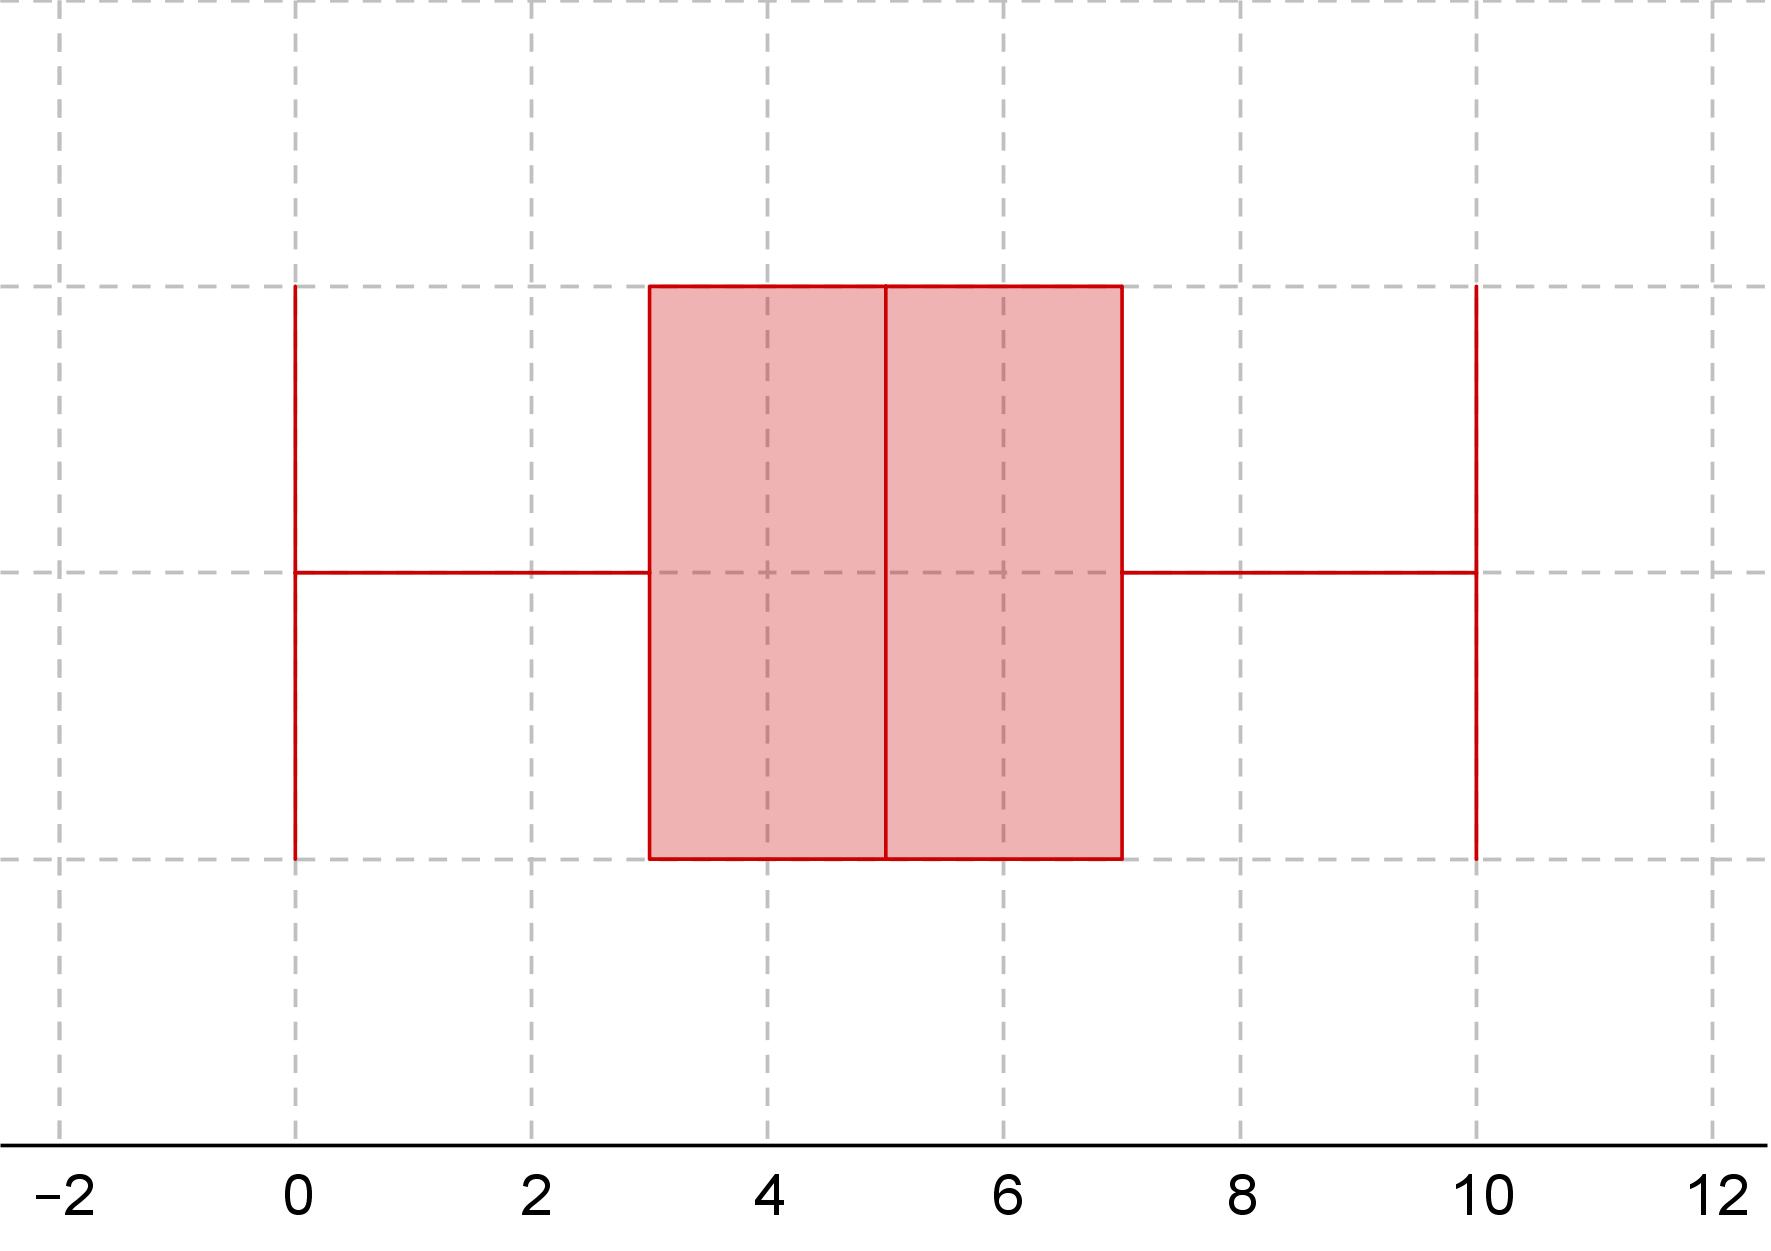
\includegraphics[width=.5\linewidth]{boxplotexercicio9.png}
\caption{Boxplot dos resultados dos candidatos na prova de seleção}
\label{}
\end{figure}
\end{enumerate}
}{9}
\end{answer}
\phantomsection\label{\detokenize{PE104-A:ativ-dadosagrupados}}
\begin{task}{ medidas para dados agrupados}

Os resultados obtidos na prova de seleção para vagas de estágio numa empresa estão representados no histograma a seguir.
\phantomsection\label{\detokenize{PE104-A:fig-hist-vagas-estagio}}
\begin{figure}[H]
\centering

\noindent\includegraphics[width=150pt]{{exercicio9}.png}
\caption{Histograma das notas na prova de seleção para vagas de estágio}
\label{\detokenize{PE104-A:fig-hist-vagas-estagio}}\end{figure}

\begin{enumerate}
\item {} 
Com base neste histograma, calcule a média, a variância, a mediana, a moda, o primeiro quartil e o terceiro quartil.

\item {} 
Usando a informação do histograma, faça um esboço do boxplot destes dados.

\end{enumerate}
\end{task}



\subsection{Um método para a determinação dos quartis}

Existem métodos diferentes para determinar os quartis de um conjunto \(\{x_1,x_2,\cdots,x_n\}\) de \(n\) observações. Um método simples será descrito a seguir.

Tome $Q_1$ como o valor correspondente à posição \(\frac{n+1}{4}\) depois de ordenar os dados.

Tome $Q_2$ como a mediana do conjunto de dados, calculada pelo método apresentado para o cálculo da mediana.

Tome $Q_3$ como o valor correspondente à posição \(\frac{3n+1}{4}\) depois de ordenar os dados.

Se os resultados de  \(\frac{n+1}{4}\) e \(\frac{3n+1}{4}\) não forem números inteiros, arredonde-os para o inteiro mais próximo. Se a parte decimal do resultado destas operações for $0{,}5$; calcule a média dos dois valores nas posições correspondentes. Por exemplo, suponha \(n=21\) tal que \((21+1)/4=5,5\). Assim, neste caso, para obter o primeiro quartil, calcule a média dos valores nas posições 5 e 6.

Vamos voltar aos dados da atividade \hyperref[\detokenize{PE104-0:ativ-notas-de-artes}]{Notas de Arte}. Como \(n=35\), para o primeiro quartil tomaremos o valor da posição \(\frac{35+1}{4}=9\), a saber, \(\text{Q}1=5\), já vimos que a mediana é $6{,}5$ e, para o terceiro quartil tomaremos o valor da posição \(\frac{3\cdot 35+1}{4}=26{,}5\). Como $26{,}5$ é equidistante das posições 26 e 27, tomaremos o terceiro quartil como a média dos dois valores nestas duas posições, a saber, \(Q_3=\frac{7,3+7,5}{2}=7,4\). Logo, podemos dizer que na turma cerca de $25\%$ das notas foram menores do que $5$ e cerca de $25\%$ das notas foram maiores do que $7{,}4$.

\subsection{Soma dos desvios da média}

Considerando o conjunto \(\{ x_1,x_2,\cdots, x_n\}\) com \(n\) observações, seja \(\bar{x}\) a média deste conjunto.  Define-se como um \index{desvio da média}desvio da média, a diferença entre uma observação e a média, a saber,
\begin{equation*}
\begin{split}d_i=x_i-\bar{x}, \quad i=1,2,\cdots, n\end{split}
\end{equation*}
Uma propriedade dos desvios da média é dada por
\begin{equation*}
\begin{split}\sum^n_{i=1}d_i=\sum^n_{i=1}(x_i-\bar{x})=0,\end{split}
\end{equation*}
qualquer que seja o conjunto \(\{ x_1,x_2,\cdots, x_n\}\).

Demonstração:

$$\displaystyle{\sum^n_{i=1}} (x_i-\bar{x})=(x_1-\bar{x})+(x_2-\bar{x})+\cdots+(x_n-\bar{x})=\\ \underbrace{(x_1+x_2+\cdots +x_n)}_{=n\cdot \bar{x}} - n\cdot \bar{x}=0$$

lembrando que \(\displaystyle\bar{x}=\frac{x_1+x_2+\cdots+x_n}{n}\).

Veja um exemplo na seção \DUrole{xref,std,std-ref}{sub-desviosdamedia}.

\subsection{Fórmula para o cálculo da variância amostral}

Vimos que a variância amostral do conjunto de dados \(\{x_1,x_2,\cdots,x_n\}\) é definida por
\begin{equation*}
\begin{split}s^2 = \frac{1}{n-1}\cdot \sum^n_{i=1} (x_i-\bar{x})^2=\frac{(x_1-\bar{x})^2+(x_2-\bar{x})^2+\cdots+(x_n-\bar{x})^2}{n-1}\end{split}
\end{equation*}
De fato, é possível mostrar que
\begin{equation*}
\begin{split}s^2 = \frac{1}{n-1}\cdot \left (\sum^n_{i=1} x^2_i-n\cdot \bar{x}^2\right )\end{split}
\end{equation*}
Demonstração:  Expandindo a soma no numerador da fórmula da variância é possível concluir que
\begin{equation*}
\begin{split}\sum^n_{i=1}(x_i-\bar{x})^2= \sum^n_{i=1} x^2_i -n\cdot \bar{x}^2\end{split}
\end{equation*}
Lembre que \((x_i-\bar{x})^2=x^2_i-2\cdot \bar{x}\cdot x_i+\bar{x}^2\). Assim,
\begin{equation*}
\begin{split} \sum^n_{i=1}(x_i-\bar{x})^2=\sum^n_{i=1}(x^2_i-2\cdot \bar{x}\cdot x_i+\bar{x}^2)=\\ (x^2_1-2\cdot\bar{x}\cdot x_1+\bar{x}^2)+(x^2_2-2\cdot\bar{x}\cdot x_2+\bar{x}^2)+ \cdots + (x^2_n-2\cdot\bar{x}\cdot x_n+\bar{x}^2)\end{split}
\end{equation*}
Como a soma é finita, podemos reunir os termos semelhantes, obtendo
\needspace{10em}
\begin{equation*}
\begin{split}\sum^n_{i=1}(x_i-\bar{x})^2= \\ (x^2_1+x^2_2+\cdots x^2_n)\underbrace{-2\cdot \bar{x}\cdot \overbrace{(x_1+x_2+\cdots+x_n)}^{=n\cdot \bar{x}}}_{=-2\cdot n\cdot \bar{x}^2}+n\cdot \bar{x}^2= \\ \sum^n_{i=1} x^2_i-n\cdot\bar{x}^2\end{split}
\end{equation*}
Vamos voltar aos dados da atividade \hyperref[\detokenize{PE104-0:ativ-notas-de-artes}]{Notas de Arte}. Temos \(n=35\), \(\displaystyle{\sum^{35}_{i=1}}x_i=207{,}5\) e \(\displaystyle{\sum^{35}_{i=1}}x^2_i=1361{,}39\)  tal que \(\bar{x}=\frac{207{,}5}{35}\approx 5{,}93\) e
\begin{equation*}
\begin{split}s^2=\frac{1}{34}\left ( 1361{,}39-35\cdot 5{,}93^2\right )\approx 3{,}8417\end{split}
\end{equation*}
tal que o desvio padrão amostral é, aproximadamente, $1{,}96$.

\subsection{Análises exploratórias bivariadas}

Em geral, nos estudos de investigação estatística, observam-se mais de uma variável para cada unidade. Quando faz sentido, investigam-se possíveis relações entre as variáveis observadas e o primeiro passo nessa investigação é a visualização dos dados observados em gráficos. Apresentaremos aqui sugestões de representações gráficas adequadas para pares de variáveis sob investigação.

Os gráficos adequados para investigar possíveis associações entre duas variáveis dependem da natureza das variáveis sob estudo que podem ser ambas quantitativas, ambas qualitativas ou uma qualitativa e outra qualitativa. Lembre-se que classificamos uma variável em quantitativa se ela assume valores numéricos e qualitativa se ela assume respostas não numéricas tal como profissão: nível médio, professor, engenheiro, advogado etc.

Vamos considerar as três situações distintas: (1) duas variáveis quantitativas, (2) duas variáveis qualitativas (categóricas) e (3) uma variável qualitativa e uma variável quantitativa, conforme os exemplos a seguir.

\clearpage
\begin{example}{Consumos de luz e de gás}
Um morador da cidade do Rio de Janeiro registrou seus consumos de gás (em metros cúbicos) e de luz (quilowatt-hora) ao longo dos meses de maio de 2019 até junho de 2020. Os dados são apresentados na tabela a seguir.

\begin{table}[H]
\centering

\begin{tabular}{|c|f|f|}
\hline
\tcolor{mês/ano} & $\tcolor{gás}$ & $\tcolor{luz}$ \\
\hline
mai/19 & 34 & 1031 \\
\hline
jun/19 & 44 & 538 \\
\hline
jul/19 & 47 & 835 \\
\hline
ago/19 & 43 & 739 \\
\hline
set/19 & 39 & 850 \\
\hline
out/19 & 31 & 1303 \\
\hline
nov/19 & 31 & 1050 \\
\hline
dez/19 & 24 & 951 \\
\hline
jan/20 & 17 & 1123 \\
\hline
fev/20 & 20 & 1202 \\
\hline
mar/20 & 25 & 1250 \\
\hline
abr/20 & 24 & 1040 \\
\hline
mai/20 & 28 & 1020 \\
\hline
jun/20 & 29 & 920 \\
\hline
\end{tabular}
\end{table}

Para visualizar o comportamento das duas variáveis simultanemanete podemos contruir o chamado diagrama de dispersão que nada mais é do que o plano cartesiano cujos $14$ pontos assinalados correspondem aos pares ordenados dados por (consumo de gás, consumo de luz) referentes aos meses de maio de 2019 até junho de 2020. Veja uma ilustração do diagrama de dispersão desses dados na \hyperref[gasluz]{figura \ref{gasluz}}.

\begin{figure}[H]
\centering

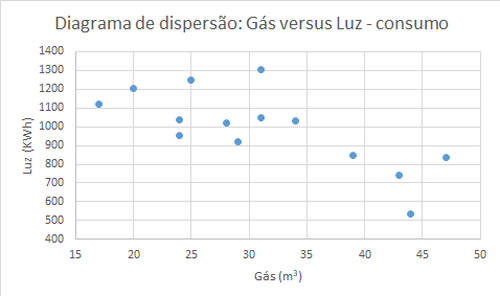
\includegraphics[width=300bp]{gasluz.png}
\caption{Diagrama de dispersão do consumo gás versus o consumo de energia}
\label{gasluz}
\end{figure}


É possível perceber, a partir do diagrama de dispersão da \hyperref[gasluz]{figura \ref{gasluz}}, uma certa tendência: a medida que o consumo de gás aumenta, o consumo de energia parece diminuir. Essa observação pode ser explicada para uma residência cujo sistema de aquecimento de água é a gás e que tem aparelhos de ar condicionado. Nesse caso, o uso de gás diminui em épocas de temperaturas mais altas devido ao menor número de banhos quentes, enquanto o consumo de energia aumenta devido ao uso mais intenso do ar condicionado. E, em épocas de temperaturas mais baixas, aumenta o consumo de gás, enquanto diminui o consumo de energia.

Observe que nesse exemplo é importante perceber que não podemos afirmar que exista uma relação de causa e efeito entre essas duas variáveis (consumo de gás e consumo de energia). De fato, a variável que afeta principalmente esses consumos é a temperatura. No entanto, outras informações sobre o local analisado também podem ajudar a explicar o comportamento dessas variáveis.

Nesse exemplo, apresentamos o diagrama de dispersão, usado para representar o comportamento conjunto de duas variáveis quantitativas.
\end{example}

\begin{example}{Mortes por COVID-19 em Nova York (2020)}
Os dados que serão trabalhados nesse exemplo são preliminares e sujeitos a variações na medida em que novos casos sejam investigados. Eles referem-se a casos de óbitos por COVID-19 de pessoas residentes na cidade de Nova York coletados até 14 de abril de 2020. Um total de $5.235$ registros de óbitos foi analisado e observaram-se a faixa de idades e o fato da pessoa ter ou não comorbidades, ou seja, ser ou não do grupo de risco (idosos, diabéticos, hipertensos etc.) Os dados foram resumidos na tabela

\begin{table}[H]
\centering

\begin{tabular}{|c|f|f|f|}
\hline
\tcolor{Faixa etária} & $\tcolor{Com comorbidades}$ & $\tcolor{Sem comorbidades}$ & $\tcolor{Total}$ \\
\hline
18 a 44 anos & 244 & 25 & 269 \\
\hline
45 a 64 anos & 1343 & 59 & 1402 \\
\hline
65 a 74 anos & 1272 & 26 & 1298 \\
\hline
75 ou mais & 2289 & 27 & 2316 \\
\hline
Total & 5148 & 137 & 5285 \\
\hline
\end{tabular}
\caption{Distribuição conjunta dos óbtiso por COVID-19 em função da faixa etária e do fato de pertencer ou não ao grupo de risco. Fonte: \href{https://www1.nyc.gov/assets/doh/downloads/pdf/imm/COVID-19-daily-data-summary-deaths-04222020-1.pdf}{NYC Health}. Acesso em junho de 2020.}
\label{mortes-COVID}
\end{table}

Observe que nessa investigação, a unidade de observação é um óbito de pessoa residente na cidade de Nova York. As variáveis observadas para cada unidade são faixa etária (qualitativa, apesar da idade ser numérica aqui elas foram agrupadas em classes) e o fato de ter ou não comorbidades (também qualitativa).

Olhando rapidamente a tabela é imediato perceber que é muito raro o óbito ocorrer para pessoas sem comorbidades, pois de um total de 5285, apenas 137 foram nesse grupo, correspondendo a apenas $2{,}62\%$ do total. É possível também perceber, que pessoas da faixa etária 18 a 44 anos tem menos chances de vir a óbito, pois apenas $269$ pessoas dessa faixa vieram a óbito de um total de $5.285$, correspondendo a $5{,}14\%$ do total.

A questão que surge para esse caso, duas variáveis qualitativas, é como representá-los em um gráfico para visualizarmos o comportamento conjunto dessas duas variáveis.

Um gráfico adequado nesse caso é gráfico de barras múltiplas representando perfis-linha ou coluna da tabela de distribuição conjunta que costuma ser chamada de tabela de dupla-entrada (ou tabela de contingência).

Por exemplo, vamos construir os perfis-coluna dessa tabela, ou seja, as distribuições percentuais de óbitos por faixa etária condicionadas aos grupos com e sem comorbidades. Veja os perfis obtidos na tabela a seguir, incluindo o perfil com todos os casos observados.

\begin{table}[H]
\centering

\begin{tabular}{|c|f|f|f|}
\hline
\tcolor{Faixa etária} & $\tcolor{Com comorbidades}$ & $\tcolor{Sem comorbidades}$ & $\tcolor{Total}$ \\
\hline
18 a 44 anos & 4{,}7 & 18{,}2 & 5{,}1 \\
\hline
45 a 64 anos & 26{,}1 & 43{,}1 & 26{,}5 \\
\hline
65 a 74 anos & 24{,}7 & 19{,}0 & 24{,}6 \\
\hline
75 ou mais & 44{,}5 & 19{,}7 & 43{,}8 \\
\hline
Total & 100 & 100 & 100 \\
\hline
\end{tabular}
\caption{Distribuição conjunta dos óbtiso por COVID-19 em função da faixa etária e do fato de pertencer ou não ao grupo de risco. Fonte: \href{https://www1.nyc.gov/assets/doh/downloads/pdf/imm/COVID-19-daily-data-summary-deaths-04222020-1.pdf}{NYC Health}. Acesso em junho de 2020.}
\label{mortes-COVID2}
\end{table}

Veja na \hyperref[fig-COVID19-est]{figura \ref{fig-COVID19-est}} 8.49 um gráfico de barras múltiplas, ilustrando os dados da \hyperref[mortes-COVID2]{tabela \ref{mortes-COVID2}}.



\begin{figure}[H]
\centering

\includegraphics[width=300bp]{COVID19.png}
\caption{Distribuições percentuais dos óbitos por faixa-etária segundo o grupo (todos, sem comorbidades e com comorbidades)}
\label{fig-COVID19-est}
\end{figure}


Podemos facilmente perceber que o grupo das pessoas com comorbidades apresenta comportamento diferente em relação aos casos por faixa etária quando comparado ao grupo sem comorbidades. No primeiro caso, $44{,}5\%$ dos óbitos ocorreram na faixa etária de 75 anos ou mais, enquanto que no segundo caso, o total de óbitos nessa faixa etária foi de $19{,}7\%$.

As diferenças observadas nos dois perfis (com comorbidades e sem comorbidades) nos levam a concluir que deve haver alguma associação entre essas duas características. No caso do grupo sem comorbidades $43{,}1\%$ dos óbitos ocorreram na faixa etária 45 a 64 anos, enquanto que no outro grupo esse percentual foi de $26{,}1\%$.

Nesse exemplo, apresentamos o gráfico de barras múltiplas usado para representar o comportamento conjunto de duas variáveis qualitativas.
\end{example}

\clearpage
\begin{example}{Maratona de Nova York (2017)}
Na \hyperref[\detokenize{PE104-0:ativ-maratona-de-ny}]{primeira atividade} desse capítulo trabalhamos com os dados da maratona de Nova York (2017), analisando os 100 melhores tempos de chegada na categoria homens e os 100 melhores tempos de chegada na categoria mulheres. Observe que nesse caso, temos duas variáveis observadas a categoria do maratonista (homem ou mulher) e o tempo de chegada. Assim tem-se uma variável qualitatica e uma variável quantitativa. Já vimos como representar dados dessa natureza para fazer comparações. Lembre-se que construímos boxplots dos 100 melhores tempos de chegada para cada categoria. Na \hyperref[boxplot-maratona-2]{figura \ref{boxplot-maratona-2}} reproduzimos novamente os boxplots.
\begin{figure}[H]
\centering
\capstart

\noindent\includegraphics[width=400bp]{{bphm_1}.png}
\caption{Boxplots dos 100 melhores tempos de chegada (em horas) na maratona de Nova York (2017) nas categorais homens e mulheres}
\label{boxplot-maratona-2}
\end{figure}
\end{example}

Resumindo, como primeiro passo em análises exploratórias de dados bivariados devemos entender a natureza das duas variáveis. Se ambas as variáveis são quantitativas, podemos começar a investigação, construindo o diagrama de dispersão (veja o exemplo consumo de gás e luz). Se ambas as variáveis são qualitativas, podemos começar, construindo o gráfico de barras múltiplas, considerando os perfis-linha ou os perfis-coluna (veja o exemplo Mortes por COVID-19 em Nova York (2020)). Finalmente, se uma das variáveis é qualitativa e a outra é quantitativa, podemos começar a investigação, construindo os boxplots da variável quantitativa para cada categoria de resposta da variável qualitativa (veja o exemplo Maratona de Nova York (2017)).

Em um problema real, em geral, mais de duas variáveis são observadas e muitas vezes queremos entender como essas variáveis se relacionam. Podemos pensar nas análises bivariadas como um primeiro passo para uma análise mais geral.
\clearpage

\def\currentcolor{cor1}
\marginpar{\vspace{.5em}}
%Página 1
\begin{answer}{Exercícios}
{\exerciselist
  \begin{enumerate}
  \item A tabela fica da seguinte forma:
  \begin{table}[H]
  \centering 

  \resizebox{.99\linewidth}{!}
  {
  \begin{tabular}{|c|c|c|c|e{.15\linewidth}|e{.15\linewidth}|}
  \hline
  \tcolor{} & \tcolor{} & \tcolor{} & \tcolor{} & \tmcol{2}{c|}{Exemplo de notas possíveis} \tabularnewline
  \hhline{*{4}{~}--}

  \tcolor{\multirow{-2}{*}{Disciplina}} & \multirow{-2}{*}{\tcolor{1\super{o}}} & \tcolor{\multirow{-2}{*}{2\super{o}}} & \tcolor{\multirow{-2}{.4\linewidth}{Soma mínima das notas nos dois últimos bimestres}} & {3\super{o}} & 4\super{o} \tabularnewline
  \hline
  Língua portuguesa & $7$ & $4$ & $17$ & $8$ & $9$ \tabularnewline
  \hline
  Física & $5$ & $4$ & $19$ & $9$ & $10$ \tabularnewline
  \hline
  Matemática & $8$ & $8$ & $12$ & $6$ & $6$ \tabularnewline
  \hline
  História & $3$ & $4$ & $21$ & \tmcol{2}{c|}{Exame Final} \tabularnewline
  \hline
  Geografia & $5$ & $5$ & $18$ & $9$ & $9$ \tabularnewline
  \hline
  Filosofia & $7$ & $9$ & $12$ & $6$ & $6$ \tabularnewline
  \hline
  Educação Física & $9$ & $8$ & $11$ & $5$ & $6$ \tabularnewline
  \hline
  Inglês & $7$ & $5$ & $16$ & $8$ & $8$ \tabularnewline
  \hline
  Química & $3$ & $7$ & $18$ & $8$ & $10$ \tabularnewline
  \hline
  Biologia & $8$ & $6$ & $14$ & $7$ & $7$ \tabularnewline
  \hline
  \end{tabular}
  }
  \end{table}

  \item O estudante deve obter as respostas dos seguintes quadros:

  \begin{table}[H]
  \centering
  \begin{tabular}{|l|c|c|c|c|c|c|}
  \hline
  \tcolor{Disciplina} & \tmcol{4}{c|}{Desvios da média} & \tcolor{Soma} & \tcolor{Desvio padrão ($s$)} \\
  \hline
  Língua portuguesa & $0$ & $-3$ & $1$ & $2$ & $0$ & $2{,}16$ \\
  \hline
  Física & $-2$ & $-3$ & $2$ & $3$ & $0$ & $2{,}94$ \\
  \hline
  Biologia & $1$ & $-1$ & $0$ & $0$ & $0$ & $0{,}82$ \\
  \hline
  \end{tabular}
  \end{table}

  \begin{table}[H]
  \centering
  
  \begin{tabular}{|*{6}{c|}}
  \hline
  \tmcol{4}{|c|}{Notas} & \tcolor{Média} & \tcolor{Mediana} \\
  \hline
  $1$ & $7$ & $7$ & $7$ & $5{,}5$ & $7$ \\
  \hline
  $5$ & $6$ & $8$ & $9$ & $7$ & $7$ \\
  \hline
  $7$ & $7$ & $7$ & $10$ & $7{,}75$ & $7$ \\
  \hline
  \end{tabular}
  \end{table}
  \end{enumerate}
}{1}
\end{answer}
\clearmargin

%Página 2
\begin{answer}{Exercícios}
{\exerciselist
  \begin{enumerate}\setcounter{enumi}{2}
  \item A primeira a firmação é verdadeira e, na segunda, os dados são insuficientes para uma conclusão.
  \begin{enumerate}
  \item Como nem todos os recrutas têm a mesma altura, se nenhum deles medisse mais de $1{,}81$m, a média seria menor do que $1{,}81$m. Logo, pelo menos um recruta tem altura maior do que $1{,}81$m. Analogamente, se nenhum recruta medisse menos de $1{,}81$m, a média seria maior do que $1{,}81$m. Logo, ao menos um recruta mede menos de $1{,}81$ m.

  \item Por exemplo, pode-se ter no grupo 51 recrutas com $1{,}81$ m, exatamente um com $1{,}80$ m e exatamente um com $1{,}82$ m, o que tornaria a sentença a falsa. No entanto, também pode-se ter 49 recrutas com 1{,}81 m, dois com $1{,}80$ m e dois com $1{,}82$ m, o que tornaria a sentença verdadeira. Portanto, os dados são insuficientes para uma conclusão.
  \end{enumerate}
  \item Com esta transformação:
  \begin{enumerate}
  \item A média do novo conjunto será dada pela média inicial acrescida da constante a, pois
  \begin{align*}
  \bar{y}&=\frac{y_1+y_2+\cdots+y_n}{n}=\frac{x_1+a+x_2+a+\cdots+x_n+a}{n}\\
  &=\frac{\sum_{i=1}^{n}x_i+n\cdot a}{n}=\frac{\sum^n_{i=1}x_i}{n}=\frac{n\cdot a}{n}=\bar{x}+a
  \end{align*}
  \item Podemos verificar que a soma dos desvios da média tomados ao quadrado é a mesma nos dois conjuntos, pois
  \begin{equation*}
  \sum^n_{i=1}(y_i-\bar{y})^2=\sum^n_{i-1}\big[\underbrace{(x_i+a)}_{=y_i}-\overbrace{(\bar{x}+a)}^{=\bar{y}}\big]^2=\sum^n_{i=1}(x_i-\bar{x})^2.
  \end{equation*}
  Portanto, a variância do novo conjunto, denotada por $s^2_y$ será igual à variância do conjunto inicial, a saber, $s^2_y=s^2$ e, assim, o desvio padrão do novo conjunto será igual ao desvio padrão do conjunto inicial, $s_y=s$.
  \item Com base nas resposatas anteriores, o coeficiente de variação do novo conjunto será dado por 
  \begin{equation*}
  CV_y=\frac{s_y}{y}\cdot100=\frac{s}{\bar{x}+a}\cdot100.
  \end{equation*}
  Logo, se $a>0$, o coeficiente de variação do novo conjunto será menor do que o coeficiente de variação do conjunto inicial. 

  Porém, se $a<0$, o coeficiente de variação do novo conjunto será maior do que o coeficiente de variação do conjunto inicial.
  \end{enumerate}
  \end{enumerate}
}{1}
\end{answer}
\begin{answer}{Exercícios}
{\exerciselist
  \begin{enumerate}\setcounter{enumi}{4}
  \item $y_i=c\cdot x_i,i=1,2,...,n.$
  \begin{enumerate}
  \item A média do novo conjunto será dada pela média inicial multiplaca pela constante $c$, pois 
  \begin{equation*}
  \bar{y}=\frac{y_1+y_2+\cdots+y_n}{n}=\frac{c\cdot x_1+c\cdot x_2+\cdots c\cdot x_n}{n}=\frac{c}{n}\cdot\sum_{i=1}^n x_i=c\cdot\bar{x}
  \end{equation*}
  \item Podemos verificar que a soma dos desvios da média tomados ao quadrado será dada pela soma original dos desvios da média elevados ao quadrado multiplicada por $c^2$, pois
  \begin{equation*}
  \sum^n_{i=1}(y_i-\bar{y})^2=\sum_{i=1}^n(c\cdot x_i-c\cdot\bar{x})^2=c^2\cdot\sum^{n}_{i=1}(x_i-\bar{x})^2.
  \end{equation*}
  Portanto, a variância do novo conjunto, denotada por $s^2_y$ será igual à variância do conjunto inicial multiplicada por $c^2$, a saber, $s^2_y=c^2\cdot s^2$ e, assim, o desvio padrão do novo conjunto será igual ao desvio padrão do conjunto inicial multiplado por $c,s_y=c\cdot s$. Lembre que estamos considerando $c>0$.
  \item Com base nas respostas anteriores, o coeficiente de variação do novo conjunto será dado por
  \begin{equation*}
  CV_y=\frac{c\cdot s_y}{c\cdot y}\cdot 100=\frac{s}{x}\cdot100. 
  \end{equation*}
  Logo, o coeficiente de variação do novo conjunto será igual ao coeficiente de variação do conjunto inicial.
  \end{enumerate}
  \end{enumerate}
}{0}
\end{answer}
\clearmargin

%Página 3
\begin{answer}{Exercícios}
{\exerciselist
  \begin{enumerate}\setcounter{enumi}{7}
  \item O primeiro passo é colocar os tempos do quadro apresentado em ordem crescente, a saber, $20{,}50<20{,}60<20{,}80<20{,}90\leq20{,}90<20{,}96$. Como o número de observações é par ($n=8$), segue que a mediana é dada por $\dfrac{x_{(4)}}{x_{(5)}}{2}=\frac{20{,}80+20{,}90}{2}=20{,}85$. A resposta correta encontra-se na opção $\titem{d)}$.
  \item A média do número de casos confirmados é dada por $\frac{1.832}{8}=229$. Logo, o número de regiões da cidade cujo número de casos confirmados é maior do que $299$ é $5$, e o número de regiões da cidade cujo número de casos confirmados é menor do que $299$ é $3$. Assim, o número de funcionários que devem ser contratados pela prefeitura é $5\cdot10+3\cdot7=71$. A resposta correta encontra-se na opção \titem{d)}.
  \end{enumerate}
}{1}
\end{answer}
\clearmargin

%Página 4
\begin{answer}{Exercícios}
{\exerciselist
  \begin{enumerate}\setcounter{enumi}{5}
  \item 
  \begin{enumerate}
  \item Concordo, pois podemos perceber que os comprimentos dos intervalos à direita são maiores:

\resizebox{\linewidth}{!}
{
  \begin{minipage}{1.1\linewidth}
  \begin{align*}
  &Q_3-\text{mediana}=13-6{,}5=6{,}5>\text{mediana}-Q_1=6{,}5-6=0{,}5\\
  &\text{Max}-Q_3=13-9=4>Q_1-\text{Min}=6-4=2\text{ e}\\
  &\text{Max}-\text{mediana}=13-6{,}5=6{,}5>\text{mediana}-\text{Min}=6{,}5=4=2{,}5.
  \end{align*}
  \end{minipage}
}
   \item Concordo, pois há assimetria à direita.
  \item Concordo: este gráfico não nos revela a existência de um intervalo de maior frequência, pois os quatro intervalos nele considerados têm frequências relativas iguais a $0{,}25$
  \item Concordo, considerando a aproximação dada por $\frac{R}{4}=\frac{13-4}{4}=\frac{9}{4}=2{,}25$
  \item Concordo, pois $DQ=Q_3-Q_1=9-6=3$ gols
  \item Concordo: o gráfico não apresenta pontos destacados. Também podemos verificar que a cerca inferior é dada por
  \begin{equation*}
  Q_1-1{,}5\cdot DQ=6-1{,}5\cdot3=1{,}5
  \end{equation*}
  e a cerca superior é dada por
  \begin{equation*}
  Q_3+1{,}5\cdot DQ=9+4{,}5=13{,}5.
  \end{equation*}
  Como o valor mínimo é $4$ e o máximo é 13, conclui-se que não existem valores atípicos
  \item Concordo, pois o \textit{boxplot} agrupou os dados em quatro intervalos de frequências relativas dadas por $0{,}25$, a saber, $[4;6[,[6;6{,}5[,[6{,}5;9[$ e $[9;13]$. Os valores dentro dos parênteses na expressão indicada correspondem aos pontos médios de cada um destes intervalos. Ou seja, esta média foi calculada com base na fórmula
  \begin{equation*}
  \sum^4_{i=1}f_i\cdot\bar{x}_i
  \end{equation*}
  \end{enumerate}
  \end{enumerate}
}{1}
\end{answer}
\begin{answer}{Exercícios}
{\exerciselist
  \begin{enumerate}\setcounter{enumi}{8}
  \item 
  \begin{enumerate}
  \item A média é dada por $\bar{x}=\frac{132}{8}\approx7{,}33$, e o desvio padrão amostral é dado por $\displaystyle\sqrt{\frac{1}{18-1}(1060-18\cdot7{,}33^2)}\approx 2{,}33$.

  Comparando a média aproximada de $7{,}5$ com a média $7{,}33$, conclui-se que o erro de aproximação é bem pequeno, representando apenas cerca de $2{,}3$\% da média obtida com a soma exata $\frac{|7{,}5-7{,}33|}{7{,}33}\approx0{,}023$. Comparando o desvio padrão aproximado de $2{,}25$ com o desvio padrão 2{,}33, conclui-se que o erro de aproximação é bem pequeno, representando apenas cerca de $3{,}4\%$ o desvio padrão obtido com as sobas exatas $\frac{|2{,}25-2{,}33|}{2{,}33}\approx0{,}034$.
  \item Nesse caso temos 20 dados, e
  \begin{equation*}
  \sum^{20}_i=1=132+5+6=143
  \end{equation*}
  tal que a média dos \textbf{recordes} nas 20 Copas do Mundo até 2014 
  é $\bar{x}=\frac{143}{20}=7{,}15$. Para o cálculo do desvio padrão temos que considerar a soma de quadrados dos 20 \textbf{recordes}, a saber, considerando as 20 Copas, temos
  \begin{equation*}
  \sum^{20}_{i=1}x^2_i=1060+5^2+6^2=1060+25+36=1121.
  \end{equation*}
  Assim, o desvio padrão amostral é dado por
  \begin{equation*}
  \sqrt{\frac{1}{20-1}(1121-20\cdot7{,}15^2)\approx2{,}28}.
  \end{equation*}
  \end{enumerate}
  \end{enumerate}
}{0}
\end{answer}
\clearmargin

%Página 5
\begin{answer}{Exercícios}
{\exerciselist
  \begin{enumerate}\setcounter{enumi}{9}
  \item É fácil ver que a moda é zero tal que $Z=0$. Somando o número de partidas jogadas vemos foram consideradas $20$ partidas. Assim, o valor da mediana é o valor que ocupa as posições centrais $10$ e $11$. Da tabela, calculando as frequências acumuladas, vemos que até $1$ gol acumularam-se $8$ partidas e até $2$ gols, acumularam-se $12$ partidas. Assim, podemos concluir que nas posições $10$ e $11$ o número de gols foi $2$, tal que a mediana$=Y=2$. A média é dada por
  \begin{equation*}
  \bar{x}=X=\frac{5\cdot0_3\cdot1+4\cdot2+3\cdot3+2\cdot4+2\cdot5+1\cdot7}{20}=\frac{45}{20}=2{,}25.
  \end{equation*}
  Logo, tem-se $Z<Y<X$ e a resposta correta encontra-se na opção \titem{e)}
  \item As figuras a seguir ilustram os respectivos histogramas (ambos na mesma escala e usando a frequência absoluta no eixo vertical) e boxplots das notas para os alunos da manhã e da tarde.
  \end{enumerate}
\begin{multicols}{2}
    \begin{figure}[H]
  \centering
  
  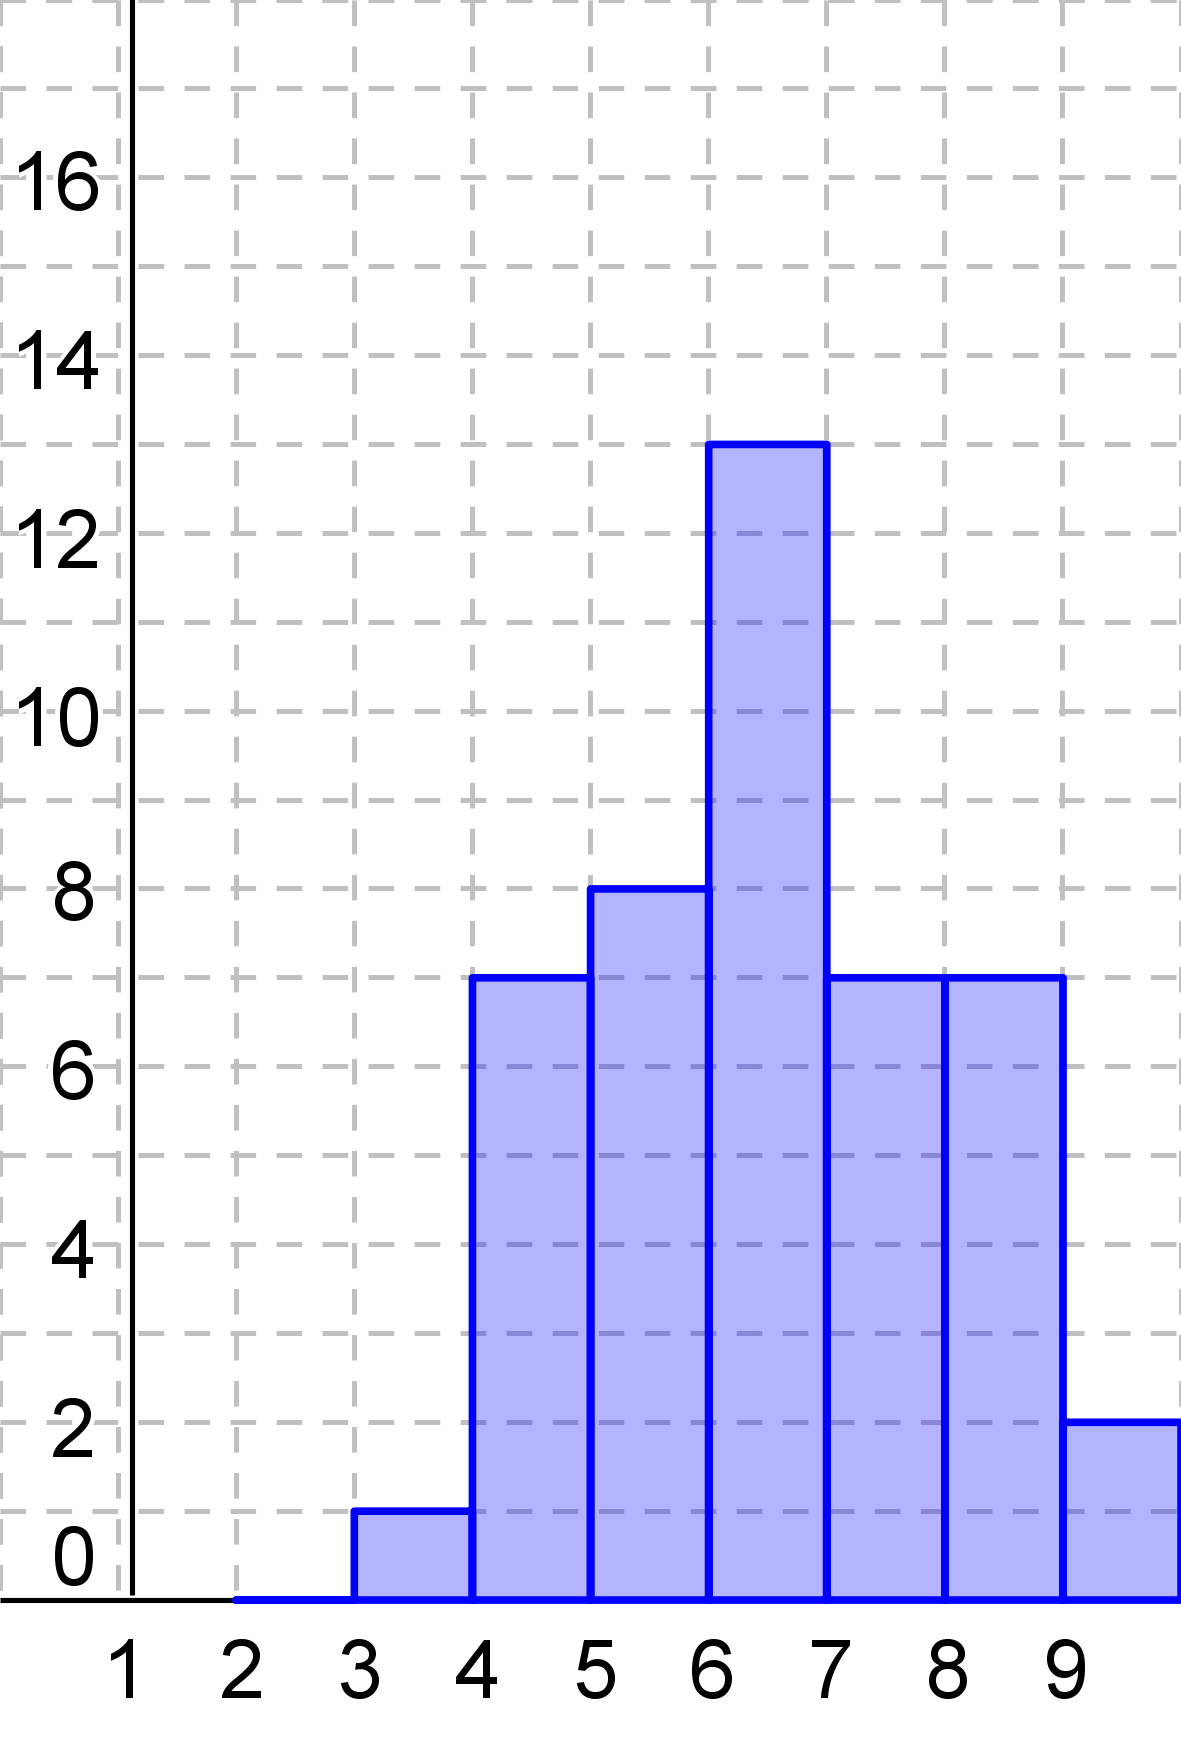
\includegraphics[width=.6\linewidth]{histograma_turma_manha_1.png}
  \caption{Histograma das notas dos alunos do turno da manhã}
  \label{}
  \end{figure}
  \begin{figure}[H]
  \centering
  
  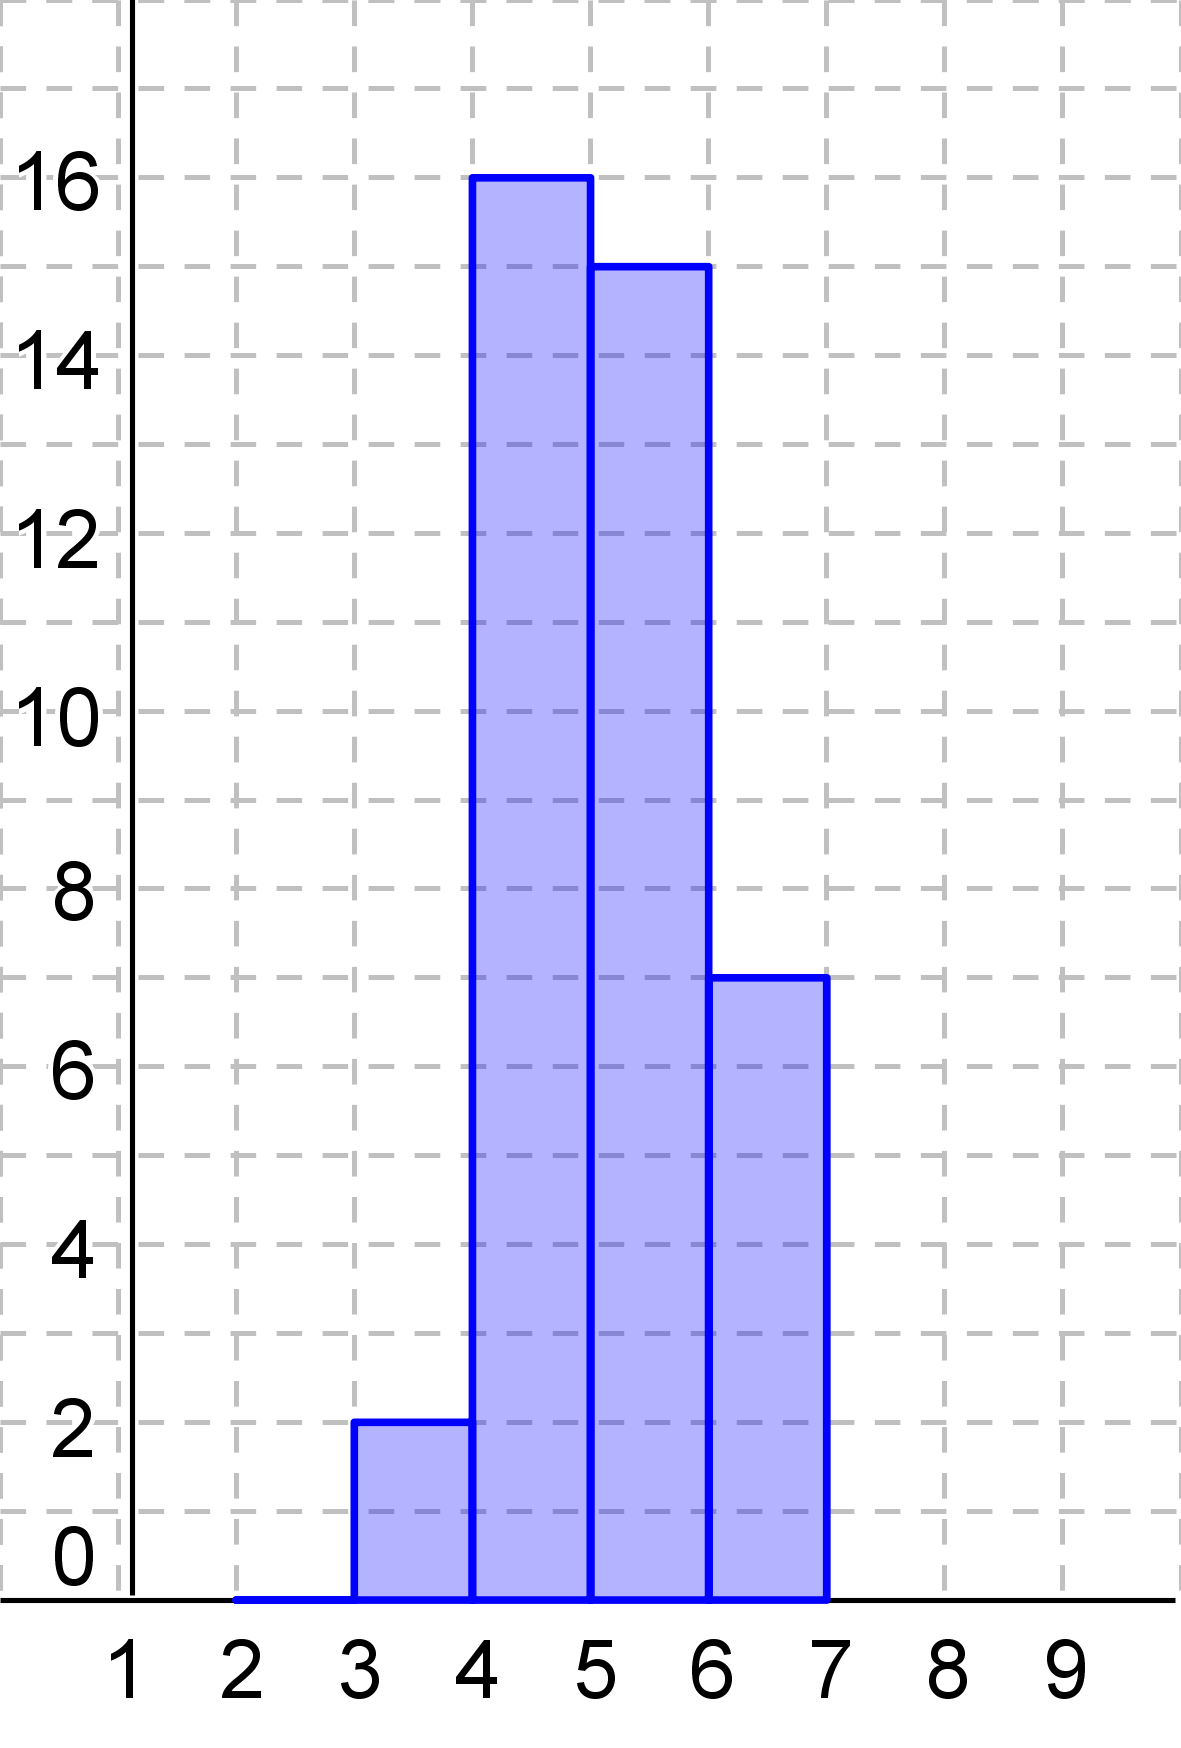
\includegraphics[width=.6\linewidth]{histograma_turma_tarde_1.png}
  \caption{Histograma das notas dos alunos do turno da tarde}
  \label{}
  \end{figure}
\end{multicols}
  \begin{figure}[H]
  \centering
  
  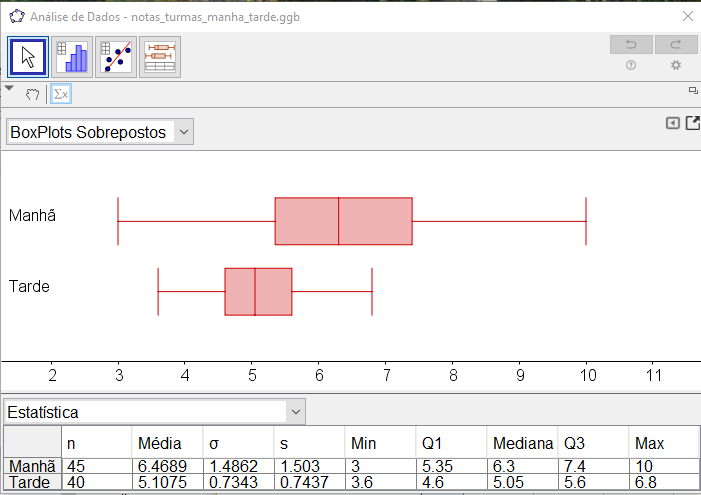
\includegraphics[width=.5\linewidth]{notas_turmas_manha_tarde.png}
   \caption{Boxplots das notas dos alunos do turno da manhã e do turno da tarde e quadro das medidas resumo gerados pelo GeoGebra}
  \label{}
  \end{figure}
}{1}
\end{answer}
\begin{answer}{Exercícios}
{\exerciselist
  \begin{enumerate}\setcounter{enumi}{10}
  \item  Comparando os dois turnos pode-se perceber que
  \begin{enumerate}
  \item ambas as distribuições de notas são aproximadamente simétricas (observe que em ambas as distribuições os valores de média e mediana são próximos, a saber, $6{,}47$ e $6{,}3$ no turno da manhã e $5{,}11$ e $5{,}05$ no turno da tarde);
  \item a dispersão das notas no turno da tarde é inferior à dispersão das notas do turno da manhã, mas o boxplot revela que o “centro”{} no turno da tarde, caracterizado pelo retângulo no boxplot está mais para à esquerda em relação ao retângulo do boxplot para os alunos do turno da manhã, indicando inferioridade de notas ($50\%$ das notas centrais no turno da tarde estão entre $4{,}6$ e $5{,}6$; enquanto que $50\%$ das notas centrais do turno da manhã estão entre $5{,}35$ e $7{,}4$);
  \item a distribuição das notas no turno da manhã é mais homogênea em relação à média do que a distribuição das notas do turno da tarde, observação que pode ser comprovada pelo cálculo do coeficiente de variação amostral de ambos os turnos, a saber, $CVA_{\text{manhã}}=\frac{1{,}503}{6{,}4686}\cdot100=23{,}2\%$ e $CVA{\text{tarde}}=\frac{0{,}7437}{5{,}1075}\cdot100=14{,}6\%$;
  \item a frequência de notas em torno da média mais ou menos um desvio padrão no turno da manhã é $62{,}2\%$ e, no turno da tarde, $70\%$ (estes valores estão perto do valor estipulado pela regra empírica de $67\%$);
  \item a frequência de notas em torno da média mais ou menos dois desvios padrões no turno da manhã é $93{,}3\%$ no turno da tarde, $92{,}5\%$ (estes valores estão perto do valor estipulado pela regra empírica de $95\%$);
  \item utilizando a aproximação grosseira para o cálculo do desvio padrão amostral, obtém-se $\frac{10-3}{4}=1{,}75$ para o turno da manhã (um erro relativo de $16{,}4\%$) em relação ao valor de $s$ calculado para o turno da manhã e, $\frac{6{,}8-3{,}6}{4}=0{,}8$ para o turno da tarde (um erro relativo de $7{,}6\%$) em relação ao valor de $s$ calculado para o turno da tarde;
  \item não existem notas atípicas nas duas distribuições;
  \item apesar do turno da manhã apresentar melhores notas, a menor nota foi observada neste turno.
  \end{enumerate}
  \end{enumerate}
}{0}
\end{answer}
\clearmargin

%Página 6
\begin{answer}{Exercícios}
{\exerciselist
  \begin{enumerate}\setcounter{enumi}{11}
  \item 
  \begin{enumerate}
  \item $I=\dfrac{3\cdot(5{,}93-6{,}5)}{1{,}945}\approx-0{,}87$, indicando alguma assimetria à esquerda.
  \item Na categoria cadeira de rodas, temos 
  \begin{equation*}
  I=\frac{3\cdot(2{,}5855-2{,}0978)}{1{,}4209}\approx1{,}03,
  \end{equation*}
  indicando alguma assimetria à direita. Na categoria mulheres temos 
  \begin{equation*}
  I=\frac{3\cdot(2{,}8698-2{,}9493)}{0{,}1867}\approx-1{,}28,
  \end{equation*}
  indicando forte assimetria à esquerda. Na categoria homens temos
  \begin{equation*}
  I=\frac{3\cdot(1{,}5116-1{,}55)}{0{,}1283}\approx-0{,}9,
  \end{equation*}
  indicando assimetria à esquerda.
  \item No turno da manhã temos
    \begin{equation*}
  I=\frac{3\cdot(6{,}4689-6{,}3)}{1{,}503}\approx0{,}3,
  \end{equation*}
  e no turno da tarde
  \begin{equation*}
  I=\frac{3\cdot(6{,}1075-5{,}05)}{0{,}7437}\approx0{,}2/
  \end{equation*}
  Pela análise dos boxplots destas duas distribuições, avaliamos que ambas eram aproximadamente simétricas. Valores de $I$ entre $-0{,}3$ e $0{,}3$ podem indicar dados aproximadamente simétricos.
  \end{enumerate}
  \end{enumerate}
}{1}
\end{answer}
\begin{answer}{Exercícios}
{\exerciselist
  \begin{enumerate}\setcounter{enumi}{12}
  \item   
  \begin{enumerate}
  \item Concordo, pois
  \begin{align*}
  \bar{y}&=\frac{1}{n}\sum^{n}_{i=1}y_i=\frac{1}{n}\sum^n_{i=1}\big[500+100\cdot(x_i-\bar{x})\big]\\
  &=\frac{1}{n}\bigg[n\cdot500=\frac{100}{s}\cdot\underbrace{\sum^n_{i=1}(x_i-\bar{x})}_{=0}\bigg]=500
  \end{align*}
  \item Concordo, pois
  \begin{align*}
  s^n_y&=\frac{1}{n-1}\sum^n_{i=1}(y_i-\bar{y})=\frac{1}{n-1}\sum^n_{i=1}\big[500+\frac{100}{s}\cdot(x_i-\bar{x})-500\big]^2)\\
  &=\frac{1}{n-1}\sum\bigg[\frac{100}{s}\cdot(x_i-\bar{x})\bigg]^2=\underbrace{\frac{100^2}{s^2}}_{\mathclap{\substack{\text{variância das} \\\text{notas originais}}}}\cdot\overbrace{\frac{1}{n-1}\cdot\sum^{n}_{i=1}(x_i-\bar{x})^2}^{=s^2}=100^2.
  \end{align*}
  Logo, o desvio padrão das notas transformadas é $s_y=\sqrt{100^2}=100$
  \item Concordo, está de acordo com a regra empírica apresentada na seção \hyperref[\detokenize{PE104-A:para-saber-mais}]{Para saber mais}: o intervalo centrado na média mais ou menos um desvio padrão corresponde às notas entre $400$ e $600$.
  \item Concordo, está de acorodo com a regra empírica apresentada na seção \hyperref[\detokenize{PE104-A:para-saber-mais}]{Para saber mais}: o intervalo centrado na média mais ou menos dois desvios padrões corresponde às notas entre $300$ e $700$.
  \end{enumerate}
  \end{enumerate}
}{0}
\end{answer}
\begin{answer}{Exercícios}
{\exerciselist
  \begin{enumerate}\setcounter{enumi}{13}
  \item 
  \begin{enumerate}
  \item \adjustbox{valign=t}
    {
    \begin{tabular}{|c|f|f|f|}
    \hline
    \tcolor{Medida} & \tcolor{X} & \tcolor{Y} & \tcolor{Z} \\
    \hline
    Média & 10 & 12 & 12 \\
    \hline
    $s$ & 1{,}487 & 2{,}81 & 0{,}725 \\
    \hline
    Min & 7 & 7 & 11 \\
    \hline
    $Q_1$ & 9 & 10 & 11{,}75 \\
    \hline
    Mediana & 10 & 12 & 12 \\
    \hline
    $Q_3$ & 11 & 14 & 12{,}25 \\
    \hline
    Max & 13 & 18 & 13 \\
    \hline
    \end{tabular}
    }
  \end{enumerate}
  \end{enumerate}
}{1}
\end{answer}
\clearmargin

%Página 7
\begin{answer}{Exercícios}
{\exerciselist
  \begin{enumerate}\setcounter{enumi}{13}
  \item 
  \begin{enumerate}\setcounter{enumii}{1}
  \item \adjustbox{valign=t}
  {
  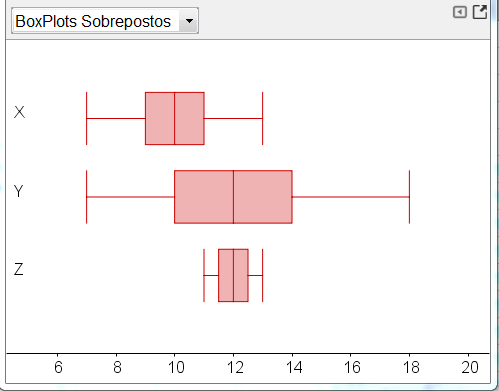
\includegraphics[width=.8\linewidth]{boxplotsmedicamentos.png}
  }
  \item Observando-se nos boxplots os comprimentos dos seguintes pares de intervalos:
  \begin{itemize}
  \item $Q_1$ e mínimo e máximo e $Q_3$;
  \item Mediana e $Q_1$ e $Q_3$ e mediana;
  \item Mediana e mínimo e Máximo e mediana.
  \end{itemize}
  conclui-se que são aproximadamente iguais, concluindo-se que as distribuições, para os três medicamentos, são simétricas. Observe que os índicens de assimetria são iguais a zero em cada uma, pois tem-se média=mediana, nas três distribuições.
  \item Como todas as distribuições são simétricas, podemos usar a regra empírica de frequ~encia entre a média mais ou menos dois desvios padrões. Para o medicamento $X$, com cerca de $95\%$ de chance a dor de cabeça será curada entre $8{,}513$min e $11{,}487$min. Para o medicamento $Y$, com cerca de $95\%$ de chance a dor de cabeça será curada entre $9{,}19$min e $14{,}81$min. Para o medicamento $Z$, com cerca de $95\%$ de chance a dor de cabeça será curada entre $11{,}275$min e $12{,}725$min. Observe que apesar do intervalo de $95\%$ de chance para o tempo de cura no medicamento em $Z$ ser mais estreito do que o mesmo intervalo para o medicamento $X$, o intervalo para o medicamento $X$ apresenta valores menores: de fato, cerca de $75\%$ dos valores em $X$ são mennores do que o valor mínimo em $Z$. Por esta razão, neste exemplo, a melhor escolha parece ser o medicamento $X$.
  \end{enumerate}
  \end{enumerate}
}{1}
\end{answer}

\exercise

\label{\detokenize{PE104-E:sec-exercicos}}\label{\detokenize{PE104-E::doc}}\label{\detokenize{PE104-E:exercicios}}

\begin{enumerate}
\item Numa Escola de Ensino Médio os estudantes precisam fazer um exame no final do ano, se a média dos bimestres for inferior a 7. Um estudante de Ensino Médio desta Escola gostaria de saber em quantas disciplinas ele pode ser aprovado sem fazer exame final. No final do segundo bimestre ele obteve as notas registradas no quadro a seguir. Indique quanto deverão somar, no mínimo, as duas notas dos dois últimos bimestres para evitar o exame final, conclua quando isto ainda é possível.

\begin{table}[H]
\centering
\begin{tabular}{|c|c|c|c|c|}
\hline
\tcolor{Disciplina} & \tcolor{1\super{o}} & \tcolor{2\super{o}} & \tcolor{Soma mínima das notas} & \tcolor{Exemplo de notas possíveis} \\
\hline
Língua portuguesa & $7$ & $4$ & & \\
\hline
Física & $5$ & $4$ & & \\
\hline
Matemática & $8$ & $8$ & & \\
\hline
História & $3$ & $4$ & & \\
\hline
Geografia & $5$ & $5$ & & \\
\hline
Filosofia & $7$ & $9$ & & \\
\hline
Educação Física & $9$ & $8$ & & \\
\hline
Inglês & $7$ & $5$ & & \\
\hline
Química & $3$ & $7$ & & \\
\hline
Biologia & $8$ & $6$ & & \\
\hline
\end{tabular}
\end{table}


\item Suponha que o aluno do exercício anterior conseguiu evitar o exame final das disciplinas de Língua Portuguesa, Física e Biologia, por ter obtido média sete. As notas deste aluno dos quatro bimestres estão indicadas no quadro a seguir.

\begin{table}[H]
\centering
\begin{tabular}{|l|c|c|c|c|}
\hline
\tcolor{Disciplina} & \tcolor{1\super{o}} & \tcolor{2\super{o}} & \tcolor{3\super{o}} & \tcolor{4\super{o}}\\
\hline
Língua portuguesa & $7$ & $4$ & $8$ & $9$ \\
\hline
Física & $5$ & $4$ & $9$ & $10$ \\
\hline
Biologia & $8$ & $6$ & $7$ & $7$ \\
\hline
\end{tabular}
\end{table}

\begin{enumerate}
\item {} 
Complete o quadro seguir com os desvios da média de cada disciplina.

\begin{table}[H]
\centering
\begin{tabular}{|l|c|c|c|c|c|}
\hline
\tcolor{Disciplina} & \tmcol{4}{c|}{Desvios da média} & \tcolor{Soma} \\
\hline
Língua portuguesa & \phantom{Soma} & \phantom{Soma} & \phantom{Soma} & \phantom{Soma} & \\
\hline
Física & & & & & \\
\hline
Biologia & & & & & \\
\hline
\end{tabular}
\end{table}


\item {} 
Em qual das disciplinas foi maior o desvio padrão das notas? E o menor?

\item {} 
Você acha que a mediana das notas seria um bom critério para a aprovação? Apresente exemplos para os quais a mediana das notas é 7 e a média é:
\begin{enumerate}[label=\roman*)]
\item {} 
inferior a 7;

\item {} 
igual a 7;

\item {} 
superior a 7.

\end{enumerate}

\end{enumerate}

\clearpage

\item (UFRJ - 2005 - adaptado)  A altura média de um grupo de 53 recrutas é $1{,}81$m. Sabe-se também que nem todos os recrutas do grupo têm a mesma altura. Diga se cada uma das afirmações a seguir é verdadeira, falsa ou se os dados são insuficientes para uma conclusão. Em cada caso, justifique a sua resposta.
\begin{enumerate}
\item {} 
“Há, no grupo em questão, pelo menos um recruta que mede mais de $1{,}81$m e pelo menos um que mede menos de $1{,}81$m.”

\item {} 
“Há, no grupo em questão, mais de um recuta que mede mais de $1{,}81$m e mais de um que mede menos de $1{,}81$m.”

\end{enumerate}

\item Seja \(\{x_1,x_2,\cdots x_n\}\) uma amostra de tamanho \(n\) de uma população, em que a média amostral é dada por \(\bar{x}\), o desvio padrão amostral é dado por \(s\) e o coeficiente de variação amostral é dado por \(\text{CV}=\frac{s}{\bar{x}}\cdot 100\%\) .

Defina um novo conjunto de dados \(\{y_1,y_2,\cdots y_n\}\) em que
\begin{equation*}
\begin{split}y_i=x_i+a,\quad  i=1,2,\cdots, n\end{split}
\end{equation*}
e \(a\) é um número real fixado, ou seja, o novo conjunto compreende todos os elementos do conjunto inicial acrescidos de uma constante \(a\) . Na atividade \hyperref[\detokenize{PE104-0:ativ-notas-de-artes}]{Notas de Arte} essa transformação será realizada sobre o conjunto das notas, se o professor acrescentar $1{,}0$ ponto às notas dos alunos da turma.
\begin{enumerate}
\item {} 
Em função da média do conjunto inicial, \(\bar{x}\), determine a média do novo conjunto.

\item {} 
Em função do desvio padrão do conjunto inicial, \(s\), determine o desvio padrão do novo conjunto.

\item {} 
Compare o coeficiente de variação do novo conjunto com o do conjunto inicial. São iguais? Por quê?

\end{enumerate}

\item Seja \(\{x_1,x_2,\cdots x_n\}\) uma amostra de tamanho \(n\) de uma população, em que a média amostral é dada por \(\bar{x}\), o desvio padrão amostral é dado por \(s\) e o coeficiente de variação amostral é dado por \(\text{CV}=\frac{s}{\bar{x}}\cdot 100\%\) . Defina um novo conjunto de dados \(\{y_1,y_2,\cdots y_n\}\) em que \(y_i=c\cdot x_i\), \(i=1,2,\cdots, n\) e \(c\) é um número real fixado e \(c>0\), ou seja, o novo conjunto compreende todos os elementos do conjunto inicial multiplicados por uma constante \(c>0.\) Na atividade \hyperref[\detokenize{PE104-0:ativ-notas-de-artes}]{Notas de Arte} essa transformação será realizada sobre o conjunto das notas, se o professor aumentar em $20\%$ a nota de cada aluno, isto é, multiplicar cada nora pelo fator $1{,}2$.
\begin{enumerate}
\item {} 
Em função da média do conjunto inicial, \(\bar{x}\), determine a média do novo conjunto.

\item {} 
Em função do desvio padrão do conjunto inicial, \(s\), determine o desvio padrão do novo conjunto.

\item {} 
Compare o coeficiente de variação do novo conjunto com o do conjunto inicial. Houve alguma alteração? Por quê?

\end{enumerate}

\clearpage
\item (ENEM 2015) Em uma seletiva para a final dos $100$ metros livres de natação, numa olimpíada, os atletas, em suas respectivas raias, obtiveram os tempos no quadro a seguir. Escolha a opção que indica o valor da mediana dos tempos apresentados.
\begin{enumerate}
\item {} 
$20{,}70$s.

\item {} 
$20{,}77$s.

\item {} 
$20{,}80$s.

\item {} 
$20{,}85$s.

\item {} 
$20{,}90$s.

\end{enumerate}

\begin{table}[H]
\centering
\caption{Tempos em segundos}
\begin{tabular}{|l|c|c|c|c|c|c|c|c|}
\hline
\tcolor{Raia} & \tcolor{1} & \tcolor{2} & \tcolor{3} & \tcolor{4} & \tcolor{5} & \tcolor{6} & \tcolor{7} & \tcolor{8} \\
\hline
Tempo(s) & 20,90 & 20,90 & 20,50 & 20,80 & 20,60 & 20,60 & 20,90 & 20,96 \\
\hline
\end{tabular}
\end{table}


\item (ENEM 2016-adaptado) Em uma cidade, o número de casos de dengue confirmados aumentou consideravelmente nos últimos dias. A prefeitura resolveu desenvolver uma ação, contratando funcionários para ajudar no combate à doença, os quais orientarão os moradores a eliminarem criadouros do mosquito Aedes aegypti, transmissor da dengue. A tabela a seguir apresenta o número atual de casos confirmados, por região da cidade.

A prefeitura optou pela seguinte quantidade de funcionários a serem contratados: (I) 10 funcionários para cada região da cidade cujo número de casos seja maior que a média dos casos confirmados e (II) 7 funcionários para cada região da cidade cujo número de casos seja menor ou igual à média dos casos confirmados. Quantos funcionários a prefeitura deverá contratar para efetivar a ação?
\begin{multicols}{5}
\begin{enumerate}
\item {} 
59

\item {} 
65

\item {} 
68

\item {} 
71

\item {} 
80
\end{enumerate}
\end{multicols}

\begin{table}[H]
\centering
\caption{Número atual de casos por região da cidade}
\begin{tabular}{|l|c|}
\hline
\tcolor{Região} & \tcolor{Casos confirmados} \\
\hline
Oeste & 237 \\ 
\hline
Centro & 262 \\
\hline
Norte & 158 \\
\hline
Sul & 159 \\
\hline
Noroeste & 160 \\
\hline
Leste & 278 \\
\hline
Centro-Oeste & 300 \\
\hline
Centro-Sul & 278 \\
\hline
Soma & 1.832 \\
\hline
\end{tabular}
\end{table}

\clearpage
\item O \textit{boxplot} a seguir representa a distribuição do número de gols da artilharia nas Copas do Mundo desde a Copa de 1930 até a Copa de 2006. Vamos chamar este número de \textbf{recorde}. Observe que só é considerado o \textbf{recorde}, sem levar em conta se houve mais de um artilheiro na Copa. Desse modo, nestas 18 Copas do Mundo, a figura leva em consideração os 18 \textbf{recordes} observados.
\begin{quote}
\phantomsection\label{\detokenize{PE104-E:fig-boxplotgols}}\begin{quote}

\begin{figure}[H]
\centering
\capstart

\noindent\includegraphics[width=100bp]{{boxpltgols}.png}
\caption{Boxplot dos \textbf{recordes} das Copas do Mundo de 1936 a 2006.}\label{\detokenize{PE104-E:id6}}\end{figure}
\end{quote}
\end{quote}

Com base neste gráfico, as seguintes afirmações foram feitas a cerca da distribuição dos \textbf{recordes}  nestas Copas do Mundo.
\begin{enumerate}
\item {} 
A distribuição apresenta assimetria à direita.

\item {} 
A média dos \textbf{recordes} é maior do que a mediana dos \textbf{recordes}.

\item {} 
O boxplot não nos permite avaliar a existência de moda.

\item {} 
Uma aproximação grosseira para o valor do desvio padrão dos \textbf{recordes} nestas Copas é dada por 2,25 gols.

\item {} 
A distância entre quartis desta distribuição é 3 gols.

\item {} 
Esta distribuição não apresentou valores atípicos.

\item {} 
Uma aproximação para o valor da média dos \textbf{recordes} pode ser calculada por \(0,25\cdot (5+6,25+7,75+11)=7,5\) gols.

\end{enumerate}

Responda se concorda ou não com cada uma destas afirmações, justificando cada resposta.

\item Na questão anterior foram consideradas 18 Copas do Mundo. Sabe-se que a soma exata dos \textbf{recordes} destas Copas é dada por \(\displaystyle{\sum^{18}_{i=1}}x_i=132\) e que a soma dos quadrados dos \textbf{recordes} é dada por \(\displaystyle{\sum^{18}_{i=1}}x^2_i=1060\).
\begin{enumerate}
\item {} 
Com base nestas informações, calcule a média e o desvio padrão dos \textbf{recordes} e compare com as aproximações obtidas no exercício anterior.

\item {} 
Consultando os \textbf{recordes} referentes às Copas de 2010 e 2014, verificou-se que eles foram 5 e 6, respectivamente. Determine a média e o desvio padrão dos \textbf{recordes}, considerando as 20 Copas do Mundo até 2014.

\end{enumerate}

\item (ENEM-2010) O quadro seguinte mostra o desempenho de um time de futebol no último campeonato. A coluna da esquerda mostra o número de gols marcados e a coluna da direita informa em quantos jogos o time marcou aquele número de gols.
\phantomsection\label{exercicio-10}
\begin{table}[H]
\centering
\caption{Desempenho de um time}
\begin{tabular}{|c|c|}
\hline
\tcolor{Gols marcados} & \tcolor{Quantidade de partidas} \\
\hline
0 & 5 \\
\hline
1 & 3 \\
\hline
2 & 4 \\
\hline
3 & 3 \\
\hline
4 & 2 \\
\hline
5 & 2 \\
\hline
7 & 1 \\
\hline
\end{tabular}
\end{table}

Se X, Y e Z são, respectivamente, a média, a mediana e a moda desta distribuição, então:
\begin{enumerate}
\item {} 
X = Y \textless{} Z                 b) Z \textless{} X = Y    c) Y \textless{} Z \textless{} X            d) Z \textless{} X \textless{} Y    e) Z \textless{} Y \textless{} X

\end{enumerate}

\item Um professor de Matemática suspeita que seus alunos do turno da tarde são mais fracos do que os seus alunos do turno da manhã. Para verificar sua suspeita, logo no início do ano letivo ele aplicou um teste básico de questões envolvendo conteúdos básicos e esperados para o nível a ser iniciado em duas amostras, uma de alunos do turno da manhã e outra de alunos do turno da tarde. A seguir, estão os resultados para as duas amostras.

\begin{multicols}{2}
\begin{table}[H]
\caption{Notas de uma amostra de alunos do turno da manhã}
\centering
\begin{tabular}{|c|c|c|c|c|}
\hline
7,4 & 7,3 & 6,2 & 6,3 & 4,1 \\
\hline
5,7 & 10,0 & 6,2 & 4,9 & 6,0 \\
\hline
8,7 & 6,5 & 3,0 & 5,8 & 7,0 \\
\hline
8,0 & 8,0 & 4,9 & 7,4 & 6,8 \\
\hline
6,7 & 7,6 & 6,1 & 6,2 & 8,5 \\
\hline
7,4 & 4,4 & 8,1 & 5,8 & 6,6 \\
\hline
4,2 & 5,3 & 4,9 & 8,1 & 6,8 \\
\hline
6,8 & 4,4 & 5,4 & 7,1 & 6,1 \\
\hline
5,3 & 5,2 & 5,7 & 9,9 & 8,3 \\
\hline
\end{tabular}
\end{table}

\columnbreak

\begin{table}[H]
\centering
\caption{Notas de uma amostra de alunos do turno da tarde}
\begin{tabular}{|c|c|c|c|c|}
\hline
5,1 & 4,7 & 5,7 & 4,7 & 5,0 \\
\hline
4,2 & 4,9 & 6,0 & 4,4 & 4,4 \\
\hline
6,0 & 4,9 & 5,6 & 6,2 & 6,6 \\
\hline
6,2 & 4,7 & 6,0 & 4,6 & 3,6 \\
\hline
5,4 & 5,2 & 5,6 & 5,5 & 5,2 \\
\hline
5,8 & 4,5 & 5,0 & 3,8 & 4,6 \\
\hline
4,1 & 4,7 & 4,2 & 6,8 & 5,6 \\
\hline
5,3 & 4,5 & 4,7 & 5,1 & 5,2 \\
\hline
\end{tabular}
\vfill
\end{table}

\end{multicols}

Usando todas as ferramentas estudadas neste capítulo, ajude este professor, fazendo um relatório detalhado e comparativo sobre os dois turnos. Se preferir, você poderá baixar estes dados no \textbf{link}, mas lembre-se que como eles estão registrados no GeoGebra, a vírgula foi trocada por ponto.

\clearpage
\item Quando comparou-se a média com a mediana falou-se em grau de assimetria da distribuição (\hyperref[\detokenize{PE104-1:sec-organizando1}]{Organizando as ideias: medidas de posição}. Na seção \hyperref[\detokenize{PE104-A:sec-para-saber-mais}]{Para saber mais} falou-se novamente em grau de assimetria. A assimetria pode ser medida pelo \textbf{índice de assimetria de Pearson}
\begin{equation*}
\begin{split}I=\frac{3\cdot(\bar{x}-\text{mediana})}{s}\end{split}
\end{equation*}
Se \(I\approx 0\), os dados são considerados aproximadamente simétricos. Um valor de \(I\) negativo, indica assimetria à esquerda e, um valor de \(I\) positivo, assimetria à direita.

Se \(I\geq 1,00\) ou \(I\leq -1,00\) , os dados podem ser considerados fortemente assimétricos à direita ou à esquerda, respectivamente. Calcule o índice de assimetria de Pearson, para os dados de
\begin{enumerate}
\item {} 
\hyperref[\detokenize{PE104-0:ativ-notas-de-artes}]{Notas de Arte};

\item {} 
\hyperref[\detokenize{PE104-7:ativ-comparacaodegruposusandoboxplot}]{Atividade: modalidades da maratona de Nova Iorque 2017};

\item {} 
\hyperref[exercicio-10]{Exercício 10}.

\end{enumerate}

\item Em provas aplicadas em grande escala é comum divulgar as notas transformadas da seguinte forma
\begin{equation*}
\begin{split}y_i = 500+100\cdot \frac{(x_i-\bar{x})}{s}, \quad i=1,2,...,n\end{split}
\end{equation*}
em que \(x_i\) é a nota obtida pelo \(i\)-ésimo candidato, \(\bar{x}=\frac{1}{n}\displaystyle{\sum^n_{i=1}}x_i\) , \(s\) é o desvio padrão amostral das notas do conjunto \(\{ x_1,x_2, ..., x_n\}\) e \(y_i\) é a nota transformada do \(i\)-ésimo candidato.

Considere as afirmações a seguir.
\begin{enumerate}
\item {} 
A média das notas transformadas é 500.

\item {} 
O desvio padrão das notas transformadas é 100.

\item {} 
Se a distribuição de notas é aproximadamente simétrica e com poucas notas atípicas, cerca de 67\% dos candidatos obtiveram notas transformadas entre 400 e 600.

\item {} 
Se a distribuição de notas é aproximadamente simétrica e com poucas notas atípicas, cerca de 95\% dos candidatos obtiveram notas transformadas entre 300 e 700.

\end{enumerate}

Responda se concorda ou não com cada uma destas afirmações, justificando cada resposta.

\item (Dados trabalhados na Atividade “Comparação de Medicamentos”{} no Capítulo \textbf{\hyperref[est1-chap]{A Natureza Estatística}})

Deseja-se comparar três medicamentos, X, Y e Z, no tratamento da dor de cabeça. Para isso 60 pacientes com perfis similares foram separados aleatoriamente em três grupos de 20 cada. Para cada grupo,  será ministrado um dos medicamentos e observado o tempo de cura da dor de cabeça (em minutos). No quadro a seguir estão dispostos os dados obtidos.

\begin{table}[H]
\centering
\begin{tabular}{|c|c|c|c|}
\hline
\tcolor{Dados ordenados} & \tcolor{X} & \tcolor{Y} & \tcolor{Z} \\
\hline
1 & 7 & 7 & 11 \\
\hline
2 & 8 & 8 & 11 \\
\hline
3 & 8 & 9 & 11 \\
\hline
4 & 9 & 9 & 11 \\
\hline
5 & 9 & 10 & 11 \\
\hline
6 & 9 & 10 & 12 \\
\hline
7 & 9 & 11 & 12 \\
\hline
8 & 10 & 11 & 12 \\
\hline
9 & 10 & 11 & 12 \\
\hline
10 & 10 & 12 & 12 \\
\hline
11 & 10 & 12 & 12 \\
\hline
12 & 10 & 12 & 12 \\
\hline
13 & 10 & 13 & 12 \\
\hline
14 & 11 & 13 & 12 \\
\hline
15 & 11 & 14 & 12 \\
\hline
16 & 11 & 14 & 13 \\
\hline
17 & 11 & 15 & 13 \\
\hline
18 & 12 & 15 & 13 \\
\hline
19 & 12 & 16 & 13 \\
\hline
20 & 13 & 18 & 13 \\
\hline
Soma simples & 200 & 240 & 240 \\
\hline
Soma de quadrados & 2042 & 3030 & 2890 \\
\hline
\end{tabular}
\end{table}

\begin{enumerate}
\item {} 
Complete o quadro a seguir.

\end{enumerate}

\begin{table}[H]
\centering
\begin{tabular}{|l|c|c|c|}
\hline
\tcolor{Medida} & \tcolor{X} & \tcolor{Y} & \tcolor{Z} \\
\hline
Média & & & \\
\hline
Moda & & & \\
\hline
$S$ & & & \\
\hline
Min & & & \\
\hline
$Q_1$ & & & \\
\hline
Mediana & & & \\
\hline
$Q_3$ & & & \\
\hline
Max & & & \\
\hline
\end{tabular}
\end{table}

\begin{enumerate}
\setcounter{enumi}{1}
\item {} 
Construa os boxplots para os três conjuntos de dados.

\item {} 
Como você avalia a forma das distribuições quanto à assimetria? Por quê?

\item {} 
Com base nas informações obtidas, que medicamento você escolheria? Por quê?

\end{enumerate}
\end{enumerate}





\section{Material Suplementar}
\label{\detokenize{PE104-E:material-suplementar}}\label{\detokenize{PE104-E:sec-applet-medidas}}
Como material de suporte para este capítulo foi desenhado um aplicativo interativo de Geogebra para a visualização de medidas de posição e dispersão de uma distribuição, que pode ser encontrado \href{https://ggbm.at/KbYqnQ6Q}{aqui}. O aplicativo pode ser usado diretamente no explorador de internet de sua preferência ou baixado e usado em computadores e celulares com \href{https://www.geogebra.org/}{Geogebra} instalado.

O aplicativo gera dados de forma aleatória, mas você pode inserir seus próprios dados na primeira coluna da planilha e verá o histograma correspondente na área gráfica, escolhendo a quantidade de partições do intervalo que você deseja.

O aplicativo permite visualizar, além do histograma, as medidas de posição da distribuição além das medidas de dispersão, mostrando: mínimo, máximo, média, mediana, $Q_1$, $Q_3$, variância e desvio padrão amostrais e populacionais.

Finalmente, é possível construir o boxplot na mesma área gráfica para que o estudante se familiarize visualmente com a relação entre o histograma e o boxplot.

\begin{figure}[H]
\centering
\capstart

\noindent\includegraphics[width=400bp]{{Aplicativo_Medidas}.png}
\caption{\href{https://ggbm.at/KbYqnQ6Q}{Aplicativo interativo em Geogebra para a visualização de medidas de posição e dispersão de uma distribuição}}\label{\detokenize{PE104-E:fig-aplicativo-medidas}}\label{\detokenize{PE104-E:id17}}\end{figure}


\ifnum\aluno=1
\clearpage
\else
\notasfinais
\fi

\bibliographystyle{apalike-pt}
\bibliography{../Bibliografia/estatistica2_bibliografia.bib}

\nocite{*}